%	Dependencies: texlive texlive-lang-german texlive-latex-recommended texlive-xetex cm-super kile biber 
%
%
%	main.tex
%
%	main for Master Thesis @ QW TU Berlin 
%
%	author: Rudolph R. Maier	
%
%	TU Berlin - 2018
%
%	Zur Benutzung von Bibtex und Biblatex: http://www.ub.uni-konstanz.de/serviceangebote/literaturverwaltung/bibtex/bibtex-und-biblatex-benutzen.html
%				Bibtex:		\renewcommand{\bibname}{Literaturverzeichnis} 
%
%	für Biber: tex.stackexchange.com/questions/26516/how-to-use-biber
% 		   pdflatex biber pdflatex
%
%% 	definiert Dokumenttyp und Grundlegende Einstellungen:
%
%
\documentclass[a4paper,oneside,11pt,titlepage,	%, captions=nooneline	% captions=nooneline --> flushleft
% pointlessnumbers,	% Kein Punkt bei Kapitelnummern, nur für scrreprt. Veraltet? (https://golatex.de/pointlessnumbers-pagestyle-t2337.html)
% draft, 		% Ggf. microtype benutzen, siehe scrguide.pdf (KOMA Script v. 20.08.2017) S.59
% twocolumn
% bibtotoc, liststotoc, % obsolete options 
% longbibliography % deprecated: bibtex option
% bibtotoc - Lit.VZ im Inha1ltsVZ
]{scrreprt}
				
\usepackage[
 	colorlinks=true,
% 	urlcolor=blue,
 	linkcolor=red,
	pdfauthor={Rudolph Ribeiro Maier},
	pdftitle={Entwicklung eines Anlaufmodells fuer das Lean Start-up},
% 	pdfsubject={The Subject},
% 	pdfkeywords={Some Keywords},
	pdfproducer={Latex with hyperref},
 	pdfcreator={pdflatex}
	bookmarks,				% PDF index
]{hyperref}
						%	KOMA Script (als Europäische  Anpassung vorzuziehen) 
% 						%	scrartcl, scrreprt, scrbook, scrlttr2

%% Codierung
\usepackage[utf8]{inputenc}			%	Codierung im Editor fuer direkte Eingabe der Sonderzeichen (WIN: latin1 oder ansinew, MAC: applemac, alt.: utf8)
\usepackage[T1]{fontenc}			%	U.A. damit Umlaute in PDF Dokumenten gefunden werden,  (T1: PostScript Type 1)
\usepackage[ngerman]{babel}			%	Anpassung der Überschriften und Silbentrennung (ngerman. english,...)
%		
%% Seitenränder
% 
\usepackage{geometry}
\geometry{
  papersize={210mm,297mm},
  left=30mm, right=30mm, top=20mm, bottom=20mm, % margins
  headsep = \baselineskip,			% Abstand zwischen Kopf und Haupttext
  footskip = \dimexpr2\baselineskip+3mm\relax,	% Abstand zwischen Haupttext und der Grundlinie des Fußes
%   showframe,					% for debugging
%   includeheadfoot,				% include head/foot in margins
  }
%   
\clubpenalty = 10000				% Disable single lines at the start of a paragraph (Schusterjungen)
\widowpenalty = 10000				% Disable single lines at the end of a paragraph (Hurenkinder)
\displaywidowpenalty = 10000


\setlength{\parindent}{0pt}			% Kein Einrücken der Absätze

% Zeilenabstand & Font
\usepackage{setspace}				% singlespacing, onehalfspacing, doublespacing. Oder \setstretch{1.25} https://texblog.org/2011/09/30/quick-note-on-line-spacing/
						% wird später für den Fließtext mit \linespread{x} definiert

% % % % % % % % % % % % % % % % % % % % % % % % % % % % % % % % % % % % % % % % % % % % % % % % % % % % % % % 
% 
%	FONT SELECTION with Math support from The LATEX Font Catalogue: www.tug.dk/FontCatalogue
% 	Test with pdffonts main.pdf
% 
% \newcommand{\changefont}[3]{
% \fontfamily{#1} \fontseries{#2} \fontshape{#3} \selectfont}
% \renewcommand{\rmdefault}{lmr}
% 
% \addtokomafont{sectioning}{\rmfamily} 		% 	Überschriften mit Serifen!
% 
% 	Latin Modern - Enhanced Computer Modern
% 
% \usepackage{lmodern}	% works: LMRoman12-Regular
% 
%
% 	EB Garamond (T1)	The default is oldstyle numbers. I have set the numbers to be lining to display lining numbers as well as oldstyle numbers
% 
% \usepackage[lining,scaled=.95]{ebgaramond} % works: EBGaramond12-Regular 		
% 
% 
% 	Garamond
% 
% \usepackage[urw-garamond]{mathdesign}	% works: GaramondNo8-Reg	 (~/texmf/fonts/type1/...)
% 
% 
% 	Nimbus Roman, is a clone of Times
% 
% \usepackage{nimbus} % ?? SFRM1200
% 
% 
% 	TIMES
% 
% \usepackage{mathptmx}	% works: NimbusRomNo9L-Regu - das hatte ich in der BA für den Fließtext
% 
% 
% 	TEX Gyre Termes, an Enhanced Time font
% 
% \usepackage{tgtermes} %	works: TeXGyreTermes-Regular 
% 
% 
% 	Palatino
% 
% \usepackage[sc]{mathpazo} % works: URWPalladioL-Roma
% \linespread{1.05}         % Palatino needs more leading (space between lines)
% 
% 
% 	KP Serif
% 
% \usepackage{kpfonts} % works: Kp-Regular
% 
% 
% 	Utopia Regular with Fourier, nur eine von beiden verwenden
% 
% \usepackage{fourier} % works: Utopia-Regular
% \usepackage[adobe-utopia]{mathdesign} % works: Utopia-Regular
% 
% 	
% 	Helvetica SANS SERIF
% 
\usepackage[scaled=0.9]{helvet}
% 
% 

\renewcommand*{\rmdefault}{\sfdefault}		% definiert serifenlos für serifenschrift (Grundtext). http://texwelt.de/wissen/fragen/785/wie-stelle-ich-alle-schrift-in-meinem-dokument-auf-serifenlos


% New header
\usepackage{scrlayer-scrpage}			% replaced fancyhdr, see: https://tobiw.de/tbdm/layout-2
\clearpairofpagestyles
 
\setkomafont{pageheadfoot}{\sffamily\footnotesize}
\setkomafont{pagehead}{\normalsize}		% {\bfseries}
\setkomafont{pagination}{}

\KOMAoptions{
   headsepline = true,
   footsepline = false,
   plainheadsepline = true, 
   plainfootsepline = false,			% no function? 
}
\automark[chapter]{chapter}			% syntax: [plainoption]{normaloption}; *{forboth}
\ihead*{\headmark}
\ohead*{\pagemark}
% \ofoot[\pagemark]{}				% Seitenzahlen unten für plain
% \ohead*{Seite~\pagemark}

% \usepackage{fancyhdr}
% \fancypagestyle{text}{%
  % flush all default styles
  \fancyhf{} 
  % Left part of the Header
  \fancyhead[LO]{\nouppercase{\leftmark}}
  % Center Part of the header
  \fancyhead[C]{}
  % Right part of the header
  \fancyhead[RO]{\thepage}
  % upper ruler
  \renewcommand{\headrulewidth}{0.4pt}
}
\fancypagestyle{plain}{%
  % flush all default styles
  \fancyhf{} 
  % Left part of the Header
  \fancyhead[LO]{\nouppercase{\leftmark}}
  % Center Part of the header
  \fancyhead[C]{}
  % Right part of the header
  \fancyhead[RO]{\thepage}
  % upper ruler
  \renewcommand{\headrulewidth}{0.4pt}
}
\fancypagestyle{fzvz}{%
  % flush all default styles
  \fancyhf{} 
  % Left part of the Header
  \fancyhead[LO]{\nouppercase{\leftmark}}
%   \fancyhead[LO]{FOOOO}
  % Center Part of the header
  \fancyhead[C]{}
  % Right part of the header
  \fancyhead[RO]{\thepage}
  % upper ruler
  \renewcommand{\headrulewidth}{0.4pt}
%   \renewcommand{\chaptermark}[1]{\markboth{#1}{}}
}

% \usepackage{titleps}				%	https://tex.stackexchange.com/questions/127972/package-fancyhdr-no-dot-behind-chapter-number-in-header
% \input{latex_settings/titleps}
% 
%% Mathematik
\usepackage{amssymb}				%	Mathematische Symbole (Pfeile etc...)
\usepackage{amsfonts}
\usepackage{amsmath}				%	Fuer Mathematische Gleichungen

\usepackage[right]{eurosym}			% 	Eurozeichen 
\usepackage{amsopn}				%	für \grad
\DeclareMathOperator{\grad}{grad}		%	für \grad

% 
%Setzt den equation-Zaehler nach jeder Section zurueck
% \numberwithin{equation}{section}	
%
%% Content Management
\usepackage{lipsum}
\usepackage{subfigure} 				%	Grafiken nebeneinander : http://www.golatex.de/zwei-bilder-nebeneinander-t1915.html
\renewcommand{\floatpagefraction}{.8}		% 	Figure Objekte erst ab x % alleine auf einer Seite ohne Text
% \begin{figure} 
%     \subfigure[Bezeichnung der linken Grafik]{\includegraphics[width=0.49\textwidth]{ordner/name1.jpg}} 
%     \subfigure[Bezeichnung der rechten Grafik]{\includegraphics[width=0.49\textwidth]{ordner/name2.jpg}} 
% \caption{Titel unterm gesamten Bild} 
% \end{figure}
\usepackage{pstricks}				% 	PSTRICKS .tex Grafiken von DIA 
\usepackage{tikz}				% 	einbinden von DIA Grafiken (PGF?)
\usepackage{graphicx}				%	einbinden von Graphiken :	\includegraphics{schachbrett.eps}
\usepackage{colortbl}				% 	Für \rowcolor[gray]{0.9} zum Einfärben von Tabellenzeilen
% \graphicspath{{img/}}
% 
\usepackage{pdfpages} 				%	PDF include : 			\includepdf[pages={5,8,10-14}]{internal_rate_of_return.pdf}
\usepackage{listings}				%	Wie \begin{verbatim} : 		\begin{lstlisting}
						%	add hypertext capabilities
% 
% disable fucking ugly boxes
\hypersetup{pdfborder = 0 0 0}
% \booktabs					%	Für die Tabellen
\usepackage{tabularx}
%\usepackage{pdflscape}				%	Querformat
%\usepackage{enumitem}				%	Für bessere nummerierungen
%
% VON MAX
%\usepackage{subfigure}                         % mehrere Graphiken in einer Abbildung
%\usepackage{float}                             % erweiterte floating Befehle
%\usepackage[section]{placeins}                 % definiert \FloatBarrier
\usepackage[locale=DE]{siunitx}	
% 
% 
\usepackage[
    backend=biber,
    style=alphabetic, 	%numeric,
    bibstyle=alphabetic,
    sortlocale=de_DE,
%     natbib=true,
    url=false, 
    isbn=false,
    doi=true,
%     defernumbers=true, % 
%     ibidtracker=context, %damit ebd. funktioniert 
%     eprint=false
]{biblatex} % Biber 
\usepackage{csquotes}				% When using babel or polyglossia with biblatex, loading csquotes is recommended to ensure that quoted texts are typeset according to the rules of your main language.
\addbibresource{main.bib}
% 	Name, Vorname: 
\DeclareNameAlias{default}{last-first}
%	Doppelpunkt nach Autor ( Anstatt Punkt)
\renewcommand*{\labelnamepunct}{\addcolon\addspace}
%
% \usepackage{german,longtable}
%

%------------------------------------------------------
% Add Glossary Functionality
\usepackage[
nonumberlist, 	% don't display page location where Term is used
acronym,      % create acronym list
toc,           % Add GLossary location to Table of Contents..
% section
]      % ..as a section/chapter (but without number!)
{glossaries}
%
% Make \gls not fragile (useful if used within \caption{})
\robustify{\gls}
\robustify{\glspl}
%
% deactivate the default . after descriptions in the Glossary
\renewcommand*{\glspostdescription}{}

\addto\captionsngerman{%						% Translation for glossaries
 \renewcommand\glossaryname{Abkürzungsverzeichnis}}			% see: https://www.mrunix.de/forums/showthread.php?65522-Glossaries-Verzeichnisbezeichnungen-umbenennen
\deftranslation[to=ngerman]{Acronyms}{Abkürzungsverzeichnis (trans)}
\deftranslation[to=ngerman]{Glossary}{Stichwortverzeichnis (trans)} 
% Let the makefile build a glossary
\makenoidxglossaries
%
% Include glossary.tex file with all the definitions
% usage: \gls{id}
%
\newglossaryentry{xxx}
{
  name=xx, 
  description={xxx}
}
%
%
\newglossaryentry{jit}
{
  name=Just-in-time, 
  description={Just-in-time-Produktion oder auch bedarfssynchrone Produktion}
}
%
%
\newglossaryentry{bmc}
{
  name=BMC, 
  description={Business Model Canvas}
}
%
%
\newglossaryentry{ishikawa}
{
  name=Ishikawa, 
  description={Ursache-Wirkungs-Diagramm}
}
%
%
\newglossaryentry{fta}
{
  name=FTA, 
  description={Fault Tree Analysis}
}
%
%
\newglossaryentry{plz}
{
  name=PLZ, 
  description={Produktlebenszyklus}
}
%
%
\newglossaryentry{pdm}
{
  name=PDM, 
  description={Produktdatenmanagement}
}
%
%
\newglossaryentry{dsm}
{
  name=DSM, 
  description={Design Structure Matrix, Methode zur Analyse von hochvernetzten Systemen}
}
%
%
\newglossaryentry{atlas}
{
  name=Atlas.ti, 
  description={Software zur qualitativen Datenanalyse}
}
%
%
\newglossaryentry{kvp}
{
  name=KVP, 
  description={Kontinuierlicher Verbesserungsprozess}
}
%
%
\newglossaryentry{pdca}
{
  name=PDCA, 
  description={Plan, Do, Check, Act}
}
%
%
\newglossaryentry{fmea}
{
  name=FMEA, 
  description={Failure Mode and Effects Analysis}%. Ein QM-Werkzeug für die systematische Bewertung von Risikofolgen.}
}
%
%
\newglossaryentry{qfd}
{
  name=QFD, 
  description={Quality Function Deployment}%. Methode zur Analyse und Darstellung von mehrdimensionalen Korrelationen}
}
%
%
\newglossaryentry{pep}
{
  name=PEP, 
  description={Produktentstehungsprozess}
}
%
%
\newglossaryentry{gps}
{
  name=GPS, 
  description={Ganzheitliche Produktionssysteme nach VDI 2870}
}
%
%
\newglossaryentry{kmu}
{
  name=KMU, 
  description={Kleine und mittelständische Unternehmen}
}
%
%
\newglossaryentry{obeya}
{
  name=Obeya, 
  description={Vereinigung aller beteiligten Personen bei der Entwicklung in einem großen Raum (Teil des Toyota Produktionssystems)}
}
%
\newglossaryentry{iot}
{
  name=IoT, 
  description={Internet of Things}
}
%
%
\newglossaryentry{erp}
{
  name=ERP, 
  description={Enterprise Resource Planning}
}
%
\newglossaryentry{ipdm}
{
  name=IPDM, 
  description={Integrierte Produktdatenmodelle}
}
%
\newglossaryentry{lsu}
{
  name=LSU, 
  description={Lean Start-up}
}
\newglossaryentry{sop}
%
{
  name=SOP, 
  description={Beginn der Serienproduktion}
}
%
\newglossaryentry{smed}
{
  name=SMED, 
  description={Single Minute Exchange of Dies}%, Methode zur Senkung von Rüstzeiten}
}
%
\newglossaryentry{heijunka}
{
  name=Heijunka, 
  description={
%(平準化),
Harmonisierung des Produktionsflusses}
}

\newglossaryentry{bspw}
{
  name=bspw.,
  description={Beispielsweise}
}
%
\newglossaryentry{mvp}
{  
  name=MVP,
  description={Minimal überlebensfähiges Produkt, engl.: Minimum Viable
Product}
}

%
%%====================================================================================================
%
%
%------------------------------------------------------
% Add Blank page Functionality
\usepackage{afterpage}
\newcommand\blankpage{%
    \null
    \thispagestyle{empty}%
    \addtocounter{page}{-1}%
    \newpage}
%     
%%====================================================================================================


% % % % % % % % % % % % % % % % % % % % % % % % % % % % % % % % % % % % % % % % % % % % % % % % % % % % % % % 
\begin{document}
%
% \changefont{ptm}{m}{n}
% 
\setcounter{page}{-1}
\pagenumbering{roman}
% % \includepdf{./img/deckblatt.pdf}
% 
% \titlehead
% {Technische Universität Berlin\\
% Fakultät V  Verkehrs- und Maschinensysteme\\
% Institut für Werkzeugmaschinen und Fabrikbetrieb IWF\\
% Fachgebiet Qualitätswissenschaft\\
% Prof. Dr.-Ing. Roland Jochem\\
% Dipl.-Ing. Robert Mies
% \\
% }
% 
% \subject{Masterarbeit}
% % 						%
% \title{Entwicklung eines Anlaufmodells für das Lean Start-up}
% % 						%
% \subtitle{\author{Rudolph Ribeiro Maier (330466)} 
% }
% 						
% \date{19.07.2018}
% 
% \maketitle

\begin{titlepage}
\begin{flushright}
\includegraphics[scale=0.4]{./img/tu-logo-eps-converted-to.pdf}\\[2.5cm] % Include a department/university logo - this will require the graphicx package
\end{flushright}

\newcommand{\HRule}{\rule{\linewidth}{0.5mm}} % Defines a new command for the horizontal lines, change thickness here

\center % Center everything on the page
 
%----------------------------------------------------------------------------------------
%	HEADING SECTIONS
%----------------------------------------------------------------------------------------

\textsc{\LARGE Masterarbeit}\\[1.5cm] % Name of your university/college
\textsc{\Large Technische Universität Berlin\\Fakultät V  Verkehrs- und Maschinensysteme}\\[0.5cm] % Major heading such as course name
\textsc{\large Institut für Werkzeugmaschinen und Fabrikbetrieb IWF\\Fachgebiet Qualitätswissenschaft\\Prof. Dr.-Ing. Roland Jochem}\\[2.5cm] % Minor heading such as course title

%----------------------------------------------------------------------------------------
%	TITLE SECTION
%----------------------------------------------------------------------------------------

\HRule \\[0.6cm]
{ \huge \bfseries Entwicklung eines Anlaufmodells \\für das Lean Start-up}\\[0.4cm] % Title of your document
\HRule \\[3cm]
 
%----------------------------------------------------------------------------------------
%	AUTHOR SECTION
%----------------------------------------------------------------------------------------
% \begin{flushleft}
\begin{tabular}{ll}
Verfasser: & Rudolph Manuel \textsc{Ribeiro Maier} \\
Studiengang: & Maschinenbau \\
% Matr.-Nr.: & 330 466 \\
E-Mail: & rudolph@ribeiromaier.de \\[1cm]
Betreuer: & Prof. Dr.-Ing. Roland \textsc{Jochem} \\
& Dipl.-Ing. Robert \textsc{Mies}
\end{tabular}\\[2cm]
 
% \end{flushleft}

 

% \begin{minipage}{0.4\textwidth}
% \begin{flushleft} \large
% \emph{Autor:} Rudolph Manuel \textsc{Ribeiro Maier} \\% Your name
% \emph{Martikel-Nr.:} 330466
% \end{flushleft}
% \end{minipage}
% ~
% \begin{minipage}{0.4\textwidth}
% \begin{flushright} \large
% \emph{Betreuer:} \\
% Prof. Dr.-Ing. Roland \textsc{Jochem}\\ % Supervisor's Name
% Dipl.-Ing. Robert \textit{Mies}
% \end{flushright}
% \end{minipage}\\


% If you don't want a supervisor, uncomment the two lines below and remove the section above
%\Large \emph{Author:}\\
%John \textsc{Smith}\\[3cm] % Your name

%----------------------------------------------------------------------------------------
%	DATE SECTION
%----------------------------------------------------------------------------------------

{\large Berlin, 19. Juli 2018}\\[2cm] % Date, change the \today to a set date if you want to be precise

%----------------------------------------------------------------------------------------
%	LOGO SECTION
%----------------------------------------------------------------------------------------

% \includepdf[scale=0.2]{./img/tu-logo-eps-converted-to.pdf}
 
%----------------------------------------------------------------------------------------

\vfill % Fill the rest of the page with whitespace

\end{titlepage}


  
  % Titelblatt der Arbeit
%   \begin{titlepage}
% 
%   \includepdf[scale=0.2]{./img/tu-logo-eps-converted-to.pdf}
% %     \includegraphics[scale=0.45]{./img/tu-logo-eps-converted-to.pdf }
%     \vspace*{2cm} 
% 
%  \begin{center} \large 
%     
%     Masterarbeit
%     \vspace*{2cm}
% 
%     {\huge Titel der Bachelorarbeit}
%     \vspace*{2.5cm}
% 
%     Name des Autors
%     \vspace*{1.5cm}
% 
%     Datum der Abgabe
%     \vspace*{4.5cm}
% 
% 
%     Betreuung: Name der Betreuerin / des Betreuers \\[1cm]
%     Fakult\"at für Mathematik \\[1cm]
% 		Karlsruher Institut für Technologie
%   \end{center}
% \end{titlepage} % This is the titlepage
\maketitle
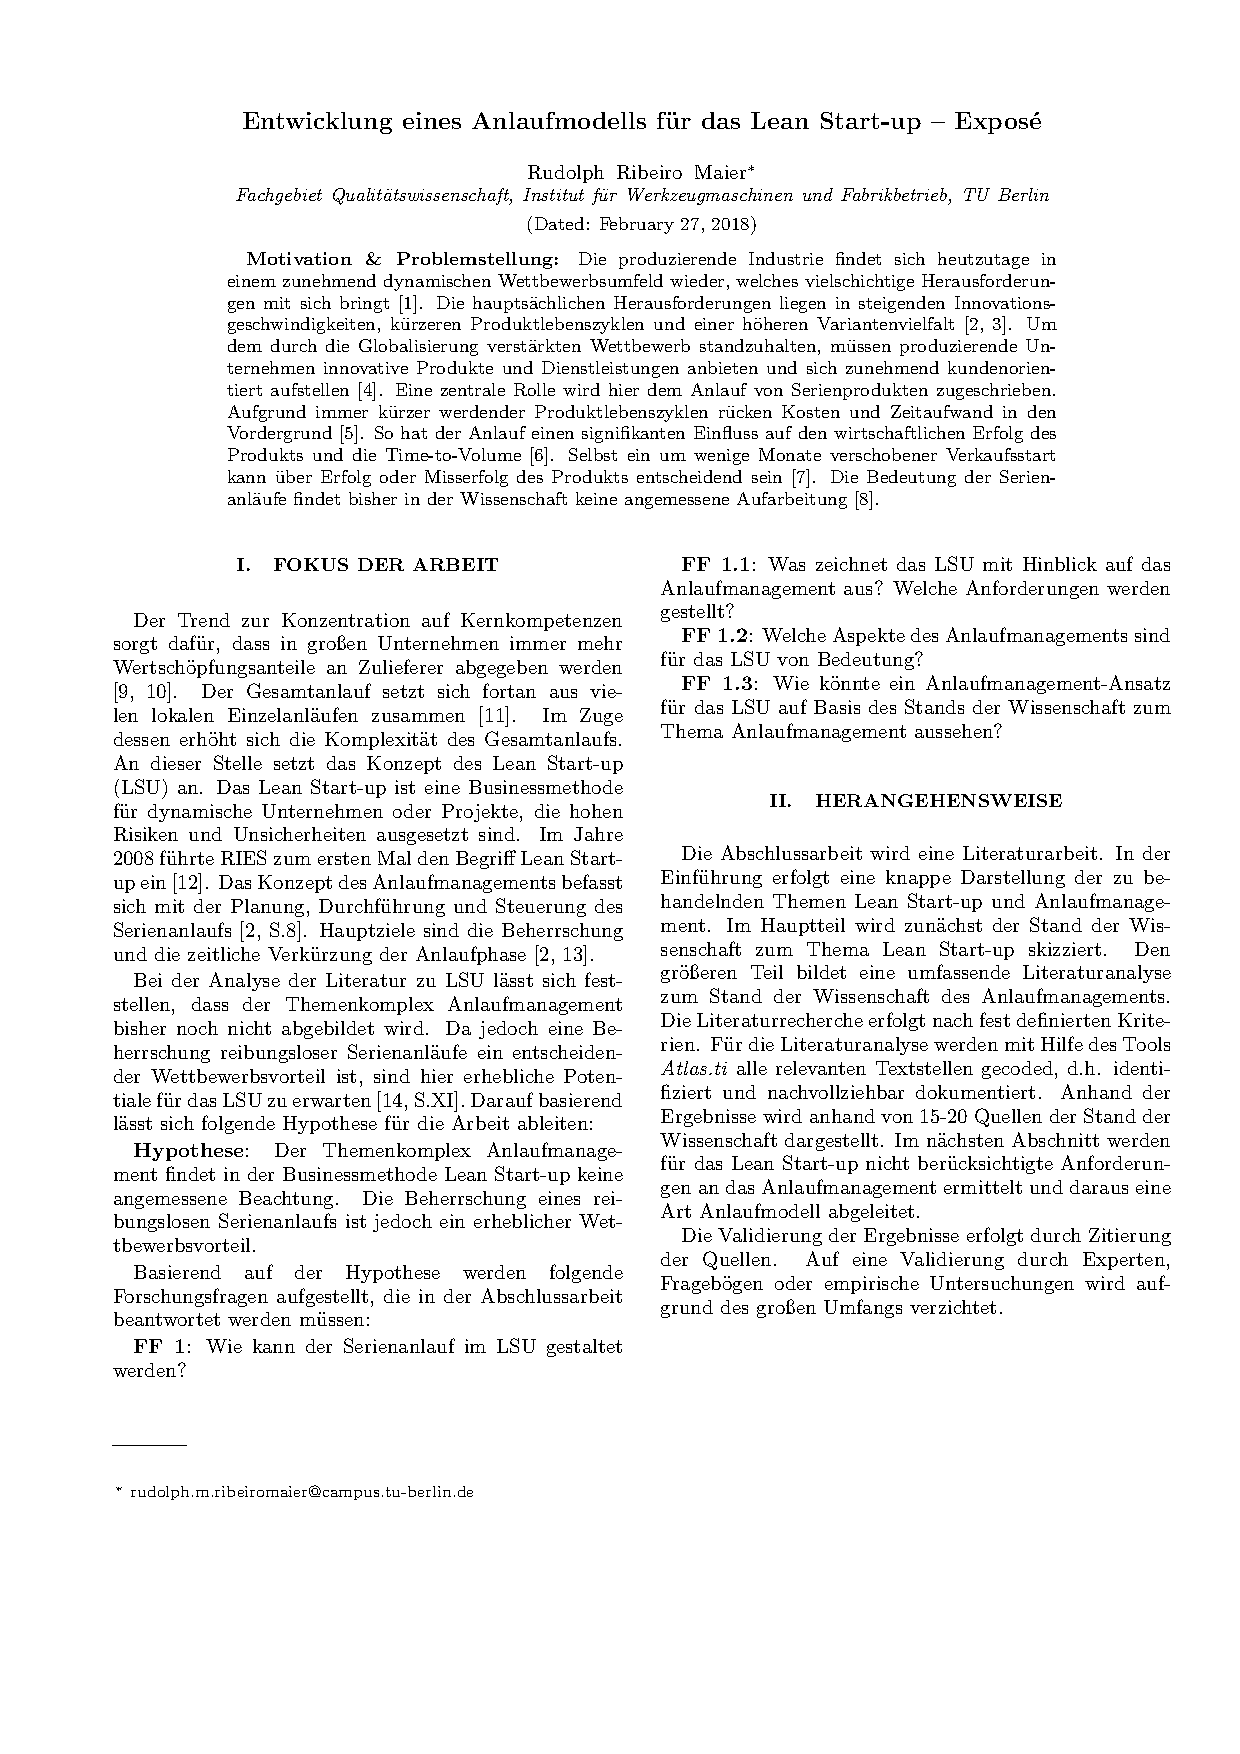
\includepdf[pages={1,2}]{latex_settings/onepager.pdf}			% Aufgabenstellung
% \includepdf[pages=2]{latex_settings/onepager.pdf}			% Aufgabenstellung
% \blankpage
%
%
%=====================================================
% Load Declaration of Authorship
\newpage
% \pagestyle{text}
\pagestyle{headings}

\thispagestyle{empty}
\section*{Eidesstattliche Erklärung}
\begin{verbatim}

\end{verbatim}
Hiermit erkl\"{a}re ich, % Rudolph Manuel Ribeiro Maier, 
dass ich die vorliegende Arbeit %, betitelt  \textit{\enquote{Design eines Energie Harvesting Moduls für autonome Energieversorgung von Bodensensoren}} 
selbstst\"{a}ndig und eigenh\"{a}ndig sowie ohne unerlaubte fremde Hilfe und ausschließlich unter Verwendung der aufgef\"{u}hrten Quellen und Hilfsmittel angefertigt habe. \\

Die selbstständige und eigenständige Anfertigung versichert an Eides statt:

\begin{verbatim}

\end{verbatim}
\hrulefill\\
\hspace*{2cm}Unterschrift
\hfill
Berlin, 19. Juli 2018

%=====================================================
%
% \include{acknowledgment}
% \include{summary}
% \newpage
% 
% \begin{abstract}
\chapter*{Zusammenfassung}
% %  Ziele / Problemstellung
% Steigende Innovationszyklen, kürzere Produktlebenszyklen und eine höhere Variantenvielfalt bilden heute die größten Herausforderungen für die produzierende Industrie. Somit bekommen Serienanläufe einen wachsenden Einfluss auf den wirtschaftlichen Erfolg des Produkts. 
% Durch die kontinuierlich sinkende Wertschöpfungstiefe setzt sich der Gesamtanlauf aus vielen Einzelanläufen zusammen. Dadurch erhöht sich die Komplexität des Gesamtanlaufs. 
Serienanläufe stellen aufgrund ihrer zunehmenden Komplexität immer größere Herausforderungen an produzierende Unternehmen. Dies gilt insbesondere für Lean Start-ups (\gls{lsu}), die oft nicht über ein systematisches Anlaufmanagement verfügen.
Gegenstand dieser Arbeit ist die Entwicklung eines Leitfadens zur optimalen Umsetzung einer Best-Practice für den Serienanlauf im \gls{lsu}.

% % Lösung: 
% GG
Da bisher in der Literatur keine einheitliche Auffassung über Anlaufmanagement im Allgemeinen herrscht, wurden zunächst fünf wichtige Quellen identifiziert. Mit Hilfe des Tools \textit{\gls{atlas}} wurden die Themenkomplexe strukturiert und konsolidiert in einem Grundgerüst abgebildet. Dieses setzt sich aus strategisch konzeptionellen und operativen Aspekten zusammen und bildet die Struktur für die weitere Arbeit. 
%  Literaturrecherche
Anhand des Grundgerüsts erfolgte eine Literaturrecherche, die den Stand der Wissenschaft bzgl. der Themenkomplexe abbildet. Es wurden geeignete Methoden und Gestaltungsempfehlungen identifiziert und in den Kontext eingeordnet. 
% Leitfaden
Schließlich wurde ein Leitfaden nach Vorbild des Business Model Canvas erstellt. Dieses soll einem Unternehmer anhand von spezifisch zu beantwortenden Fragen helfen, zielgerichtet fundierte Entscheidungen hinsichtlich der Gestaltung eines Serienanlaufs zu treffen. 
% 

% % Impact
% Wissenschaft
Das hier entwickelte Grundgerüst sowie der Leitfaden können als Grundlage für weitere Forschung dienen. Diese kann sowohl hinsichtlich Quantität (\gls{bspw} weitere Literaturrecherche) als auch hinsichtlich Qualität (Erweiterung des Grundgerüsts) variiert werden. Denkbar ist auch eine Änderung der Betrachtungsebene. Für die wissenschaftliche Validierung der Erkenntnisse bietet sich empirische Forschung oder Ac­tion-Re­search an. 
% Bemerkung zu allg. Handlungsempfehlungen. Ggf. zu viel für das Abstract??
Weiterhin ist zu beachten, dass der Leitfaden lediglich zu gestaltende Aspekte abbildet. Im Hauptteil sind jedoch viele allgemeine Handlungsempfehlungen identifiziert worden, welche im Leitfaden nicht darstellbar sind. Diese sind jedoch von großem Interesse uns sollten \gls{bspw} in einem \textit{Handbuch Anlaufmanagement für das \gls{lsu}} zusammengefasst werden.
% 
% Wirtschaft
In der Praxis ermöglicht der Leitfaden kaufmännisch geprägten Gründern fundierte Entscheidungen zu treffen. Voraussetzungen dafür sind eine hohe Motivation sowie vorhandene Ressourcen. Ebenfalls ist ein Verständnis der Grundbegriffe aus Produktion und Qualitätsmanagement erforderlich. 
%  2061 characters

\chapter*{Abstract}
Manufacturing ramp-ups challenge the manufacturing industry due to growing complexity. This affects especially the Lean Startup (\gls{lsu}), since it doesn't have a systematically set up ramp-up management. The purpose of this Thesis is to develop a guideline which supports the setup of a proper ramp-up management in \gls{lsu}s. 

Since there is no uniform interpretation of ramp-up management in literature, five relevant sources were identified. Supported with the tool \textit{\gls{atlas}}, these five interpretations were structured and unified into a basic framework. It consists of strategic-conceptual and operational elements and provides the structure for the further work of the thesis. The literature research was based on this framework, and represents the current state of science and technology. Suitable methods and design recommendations were identified and put in context. Finally, the results were formulated into a guideline, which follows the design of the \textit{Business Model Canvas}. This guideline contains specific questions, which lead to profound decisions regarding the design of the ramp-up, when answered by the entrepreneur. 

Both the developed framework and the guideline may also provide a frame for further research. % As well...as
The research may be continued in quantitative (e.g. further research depth) as well as qualitative (expanding the framework) aspects. Additionally, the level of abstraction may be changed. Both empirical research and action research are applicable for validation of the results proposed in this Thesis. 
On the other hand, the guideline allows commercial oriented entrepreneurs to take profound decisions in their industial practice. A high level of motivation and available ressources are requirements that need to be met. In addition, the entrepreneur needs to have a basic knowledge of quality management and manufacturing terms. 

% 1870 characters
\addcontentsline{toc}{chapter}{Kurzzusammenfassung}
% \end{abstract}

\tableofcontents
%
% %=====================================================
% Print Glossary
\newpage
% \pagestyle{glossary}
% \glsaddall
\printnoidxglossaries 							% see [glossariesbegin.pdf, p.16]
% \addcontentsline{toc}{chapter}{Abkürzungsverzeichnis}
% %
% %=====================================================
% \pagestyle{fzvz}
% % \renewcommand{\chaptermark}[1]{\markboth{#1}{}}
% \newpage
% \chaptermark{Verzeichnis der Formelzeichen}	% für chaptername im fancyheader, nur hier nötig
% \addcontentsline{toc}{chapter}{Verzeichnis der Formelzeichen}
% \input{./tab/fvz1}
% \newpage
% \input{./tab/fvzg1}
% \newpage
% % \addcontentsline{toc}{chapter}{\listfigurename}
% \listoffigures
% \newpage
% \listoftables
% 
%%====================================================================================================
%             				 TEXTANFANG
%%====================================================================================================
%
% \linespread{}

% \pagestyle{text}
% Add Left Header
%
\setstretch{1.5}		% is equivalent to MS Word Zeilenabstand 1.5
%
% \include{0_work}
\newpage
\setcounter{page}{0}
\pagenumbering{arabic}
 % \section{Einführung}
\chapter{Einführung}
\section{Motivation \& Problemstellung}
Die produzierende Industrie findet sich heutzutage in einem zunehmend dynamischen Wettbewerbsumfeld wieder, welches vielschichtige Herausforderungen mit sich bringt \cite{Renner2012}. Die hauptsächlichen Herausforderungen liegen in steigenden Innovationsgeschwindigkeiten, kürzeren Produktlebenszyklen und einer höheren Variantenvielfalt \cite{Kuhn2002,Stauder2016}. Um dem durch die Globalisierung verstärkten Wettbewerb standzuhalten, müssen produzierende Unternehmen innovative Produkte und Dienstleistungen anbieten und sich zunehmend kundenorientiert aufstellen \cite{Surbier2014}. 
Eine zentrale Rolle wird hier dem Anlauf von Serienprodukten zugeschrieben. Aufgrund immer kürzer werdender Produktlebenszyklen rücken Kosten und Zeitaufwand in den Vordergrund \cite{Winkler2007}. So hat der Anlauf einen signifikanten Einfluss auf den wirtschaftlichen Erfolg des Produkts und die Time-to-Volume \cite{Klocke16}. Selbst ein um wenige Monate verschobener Verkaufsstart kann über Erfolg oder Misserfolg des Produkts entscheidend sein \cite{Schuh2008a}. Die Bedeutung der Serienanläufe findet bisher in der Wissenschaft keine angemessene Aufarbeitung \cite{Dyckhoff2012}. 

\section{Fokus der Arbeit}
Der Trend zur Konzentration auf Kernkompetenzen sorgt dafür, dass in großen Unternehmen immer mehr Wertschöpfungsanteile an Zulieferer abgegeben werden  \cite{Hilmola2015, Wildemann2008}. Der Gesamtanlauf setzt sich fortan aus vielen lokalen Einzelanläufen zusammen \cite{Zimolong2006}. Daraus resultieren höhere Abhängigkeiten zwischen größeren Unternehmen und den Zulieferern, die meist mittelständische Unternehmen sind. 

Die Abschlussarbeit soll sich im Speziellen mit dem Serienanlauf im KMU und SME als Zulieferer für größere Unternehmen beschäftigen, da hier erhebliches Verbesserungspotential erkennbar ist \cite[S.18]{Dombrowski2009a}. So gibt es in KMU meist keine Anlaufprozesse. Da es in KMU oft keine Stabsstellen gibt, werden Anläufe von den Mitarbeitern oft zusätzlich zum Tagesgeschäft gesteuert \cite{Dombrowski2009}. %TODO kein Zugriff auf Primärquelle D.Spath!! 
Mangelnde finanzielle und zeitliche Kapazitäten sowie fehlendes Know-how verhindern eine nachvollziehbare Dokumentation sowie proaktive Maßnahmen \cite{Zimolong2006,Dombrowski2009a}. 

Weiterhin soll untersucht werden, wie der Auftraggeber den Anlaufprozess des Lieferanten unterstützen kann. Größere Unternehmen verfügen in der Regel über mehr Ressourcen und teilweise eigene Anlaufprozesse. Im Zuge der Verlagerung der Wertschöpfungsanteile, gewinnt die Innovationskraft von Modul- und Systemlieferanten zunehmend an Bedeutung für den Erfolg eines Produktes \cite{Kuhn2002}. Ein erfolgreiches und effizientes Anlaufmanagement in KMU ist im Sinne der Entwicklung einer nachhaltigen Partnerschaft für Auftraggeber und Lieferant von großer Bedeutung. \textit{Wildemann} erkennt hier das Potenzial von Einspareffekten sowie Nutzung erheblicher Wettbewerbsvorteile auf beiden Seiten \cite{Wildemann2008}.

\textit{Dyckhoff} und \textit{Scholz} sind zu der Erkenntniss gekommen, dass das Thema weder in Industrie noch in der Wissenschaft hinreichend Beachtung findet \cite{Dyckhoff2012, Scholz2010}, weshalb hier keine zufriedenstellenden Ergebnisse zu erwarten sind.
Ziel der Arbeit ist, einen Überblick über den Stand der Forschung zu geben und einen Entwurf für ein Anlaufmodell zu entwickeln. 

\section{Herangehensweise}
Die Abschlussarbeit wird eine Literaturarbeit. In der Einführung erfolgt eine knappe Darstellung der zu behandelnden Themen Lean Startup / KMU und Anlaufmanagement. Im Hauptteil wird zunächst der Stand der Wissenschaft zum Thema Lean Startup skizziert. Den größeren Teil bildet eine umfassende Literaturanalyse zum Stand der Wissenschaft des Anlaufmanagements. Die Literaturrecherche erfolgt nach fest definierten Kriterien. Für die Literaturanalyse werden mit Hilfe des Tools \textit{Atlas.ti} alle relevanten Textstellen gecoded, d.h. identifiziert und nachvollziehbar dokumentiert. Anhand der  Ergebnisse wird anhand von möglichst vielen Quellen der Stand der Wissenschaft dargestellt. Im nächsten Abschnitt werden für das Lean Startup nicht berücksichtigte Anforderungen an das Anlaufmanagement ermittelt und daraus eine Art Anlaufmodell abgeleitet. 

Die Validierung der Ergebnisse erfolgt durch Zitierung der Quellen. Auf eine Validierung durch Experten, Fragebögen oder empirische Untersuchungen wird aufgrund des großen Umfangs verzichtet.
%
\section{Kontext}

\subsection{Lean Start-up}
\subsubsection*{Einführung}
Das Lean Start-up ist eine Businessmethode für dynamische Unternehmen oder Projekte, die hohen Risiken und Unsicherheiten ausgesetzt sind. 
Hauptziele der Methode sind kürzere Entwicklungszeiten, Einsparung von Kosten in der Entwicklungsphase und frühzeitiges Erkennen der Kundenbedürfnisse. 
Sie ist eine Antwort auf hoch dynamische Märkte, unbekannte Problemstellungen und Lösungen und hohen Risiken. Die Ursprünge liegen in den Denkweisen von Taiichi Ōno, W. Edwards Deming und Peter Drucker. 
2008 übertrug Eric Ries Lean Produktions Methoden auf hochtechnologie Startups und veröffentlichte 2011 die erstmals "Lean Startup" genannte Methode in seinem Buch. %TODO 2011 or 2008? 

%\subsection*{Definitionen}

\subsubsection*{Bestandteile}

\textit{1. Entwickeln einer Vision}. Die Vision dient als Grundlage für alle weiteren Handlungen. Aus ihr werden im nächsten Schritt Hypothesen abgeleitet. Anstatt einen aufwändigen Businessplan zu erstellen wird die Vision in einem Business Model Canvas definiert \cite{Blank2013}. Die Vision eines Lean Start-up zeichnet sich durch viele Freiheitsgrade und Unsicherheiten aus. 

\textit{2. Überführen der Vision hin zu Hypothesen}. Für jedes Element der im Business Model Canvas beschriebenen Vision werden Hypothesen abgeleitet. Die Hypothesen bilden die Freiheitsgrade und Unsicherheiten des BMC ab. Ziel ist, die Risiken durch spätere Beantwortung der Hypothesen zu minimieren. Nach Möglichkeit sollen die Hypothesn so formuliert werden, dass sie quantitativ beurteilt werden können. Die Hypothesen müssen wiederlegbar sein, um neue Erkenntnisse gewinnen zu können. 

\textit{3. Entwickeln von MVP Tests}. Ein minimal überlebensfähiges Produkt (\gls{mvp}, engl.: Minimum Viable Product) ist ein Werkzeug, mit dem man schnellstmöglich die Hypothesen am Kunden überprüfen kann \cite[93]{Ries2011}. Ziel ist zum einen den Build-Measure-Learn Zyklus zu beschleunigen, zum anderen die Lernrate in Bezug auf den Aufwand zu maximieren. So können frühzeitig nicht benötigte Funktionen und Produkteigenschaften erkannt und Zeit und Kosten gespart werden. Wenn die Entwicklung eines realen MVP zu aufwändig ist, kann ein Smoke Test eingesetzt werden. In einem Smoke Test wird das zukünftige Produkt in einem Video oder über eine Webseite vorgestellt.

\textit{4. Planung der Tests}. Bei der Durchführung der Tests kommt es darauf an, Kosten und Zeit zu minimieren. Daher werden zuerst Tests durchgeführt, die wenig kosten und hohe Risiken untersuchen. Beispielsweise ist eine Patentrecherche kostengünstig und kann frühzeitig sehr hohe Risiken aufdecken. Tests können nacheinander (seriell) oder gleichzeitig (parallel) durchgeführt werden. Bei parallelen Tests riskiert man, dass einzelne Tests überflüssig werden, profitiert jedoch von einem Zeitvorsprung gegenüber der seriellen Vorgehensweise. 

\textit{5. Interpretation der Ergebnisse}. Bei der Interpretation der Ergebnisse gibt es einige Fehlerquellen. Zum einen gibt es teilweise große Differenzen zwischen den geäußerten und reellen Kundenrückmeldungen. Zum anderen kann die Interpretation des Unternehmers durch eigene Wünsche oder Erwartungen verzerrt sein.

\textit{6. Reaktion}. Nach Auswertung der Ergebnisse sieht die LSU Methode eine Entscheidung zwischen drei Handlungsalternativen vor. \textit{Preserve}: Wenn die Tests die Hypothesen bestätigen wird die Strategie beibehalten. \textit{Pivot}: Wenn die Tests die Hypothesen wiederlegen oder neue Chancen aufzeigen, wird die Strategie angepasst. \textit{Perish}: Wenn die Tests die Hypothesn wiederlegen und der Unternehmer keine geeignete Strategie entwickeln kann, wird die Strategie verworfen. 

\textit{7. Skalierung und kontinuierliche Verbesserung}. Sobald alle relevanten Hypothesen bestätigt wurden, ist das Produkt auf den Markt abgestimmt. Jetzt kann massiv in Kundenakquise und Produktentwicklung investiert werden. Wichtig ist weiterhin, dass die Strategie fortwährend überprüft wird. Ein \textit{Pivot} ist auch nach der Skalierung bei größeren Änderungen sinnvoll. 

% \subsection*{Grenzen der Methodik}

\subsection{Anlaufmanagement}
Immer kürzere Produktlebenszyklen bei gleichzeitig höher werdenden Kundenwünschen und größerer Variantenvielfalt erhöhen die Komplexität und somit die Bedeutung des Serienanlaufs \cite{Kuhn2002,Schuh2004}. Die Risiken im Zusammenhang mit der Anlaufphase sind vielfältig. KUHN %TODO Biblatex Cite command for cap letter author in maintext
stellt fest, dass der Aufwand bis zum Erreichen einer stabilen Produktion oft unterschätzt wird. Infolgedessen kann es zum verspäteten Markteintritt sowie unzureichenden Kapazitäten und Qualitätsmängeln kommen \cite{Kuhn2002}. Um diesen Risiken entgegen zu wirken werden als übergeordnete Hauptziele für das Anlaufmanagement Beherrschung und zeitliche Verkürzung der Anlaufphasae genannt \cite{Kuhn2002, Schmitt2015}. 

Produktionsanläufe stellen auch deshalb eine große Herausforderung für Unternehmen dar, da sie hochkomplex sind und sich durch viele parallele und sequenzielle Teilprozesse auszeichnen. Sie sorgen zudem für eine starke Vernetzung der beteiligten Abteilungen innerhalb und außerhalb des Unternehmens \cite{Schuh2004}.


\subsubsection*{Definition}
In der Literatur existiert keine Einheitliche Definition des Begriffs Anlaufmanagement \cite[4]{Bischoff2007}. Selbst SCHMITT %TODO 
bemängelte 2015 ein fehlendes einheitliches Verständis der grundlegenden Begriffe des Produktionsanlaufs \cite[1]{Schmitt2015}. Vielmehr existieren unternehmensintern und teilweise auch projektspezifisch unterschiedliche Auffassungen über die Definition der Anlaufphase \cite[11]{Grosshenning2005}. KUHN %TODO
definierte das Anlaufmanagement wie folgt \cite[8]{Kuhn2002}: 
\begin{quotation}
Das Anlaufmanagement eines Serienproduktes umfasst alle Tätigkeiten und Maßnahmen zur Planung, Steuerung und Durchführung des Anlaufes mit den dazugehörigen Produktionssystemen, ab der Freigabe der Vorserie bis zum Erreichen einer geplanten Produktionsmenge, unter Einbeziehung vorgelagerter Prozesse und der nachgelagerten Prozesse im Sinne einer messbaren Eignung der Produkt- und Prozessreife.
\end{quotation}
SCHUH übernahm diese Auffassung \cite{Schuh08a} während RISSE und BISCHOFF den Beginn bereits nach der abgeschlossenen Produktentwicklung sehen \cite{Risse2002, Bischoff2007} (Freigabe Pflichtenheft).

Der Anwendungsbereich beschränkt sich nicht nur auf den Anlauf von neuen Produkten. Auch Modellderivate (Modellpflege), Varianten; neue Produktionssysteme, Fertigungsverfahren und Logistikprozesse stellen aus Perspektive des Managements ein Anlauf dar \cite[6]{Bischoff2007}. %TODO cite primara source LAICK/Warnecke/Aurich 2003

\subsubsection*{Lieferanten}

Ziele Werte Verhaltensnormen für Zusammenarbeit mit Lieferanten werden gemäß der Vision definiert Schmitt2015

Harmonisierung der Schnittstellen innerhalb der SC mit transparenten unternehmensübergreifende Strukturen Bischoff2007

Gemeinsame Informationsstrategie  Kuhn02

Frühe Einbindung und Integration der Lieferanten bedeutend für reibungslosen Anlauf Bischoff2007 S.28, Kuhn2002 S. 26

Einheitliche Datenbasis für den austausch von Informationen und Planungsdaten Kuhn02

Werkzeuge: 
  Lieferanten-Audits, KVP, PDCA Schuh08
  FMEA, QFD, Ishikawa, FTA Bischoff2007

\subsubsection*{Logistik}

Die Logistik beinhaltet die Koordinierung aller Material- und Informationsflüsse und Prozesse von Auftrag bis Auslieferung des Endprodukts. Die strategische Ebene beinhaltet die Entwicklung und Gestaltung der Wertschöpfungsnetzwerde und Prozesse nach logitsischen Prinzipien. Die operative Ebene beinhaltet die Lenkung und Kontrolle der Material- und Informationsflüsse und der dazugehörigen Prozesse. 
Hauptziele der Logistik ist, durch Gestaltung und Lenkung der logistischen Prozesse die Kundenbedürfnisse in den ökologischen, ökonomischen und sozialen Dimensionen optimal zu erfüllen \cite[28]{Schmitt2015}. 

Die Bedeutung der Logistik für die Anlaufphase ist durch die Globalisierung der Märkte, JiT-Konzepte und Reduzierung der Wertschöpfungstiefe gestiegen. Die Logistik hat zwei spezielle Funktionen in der Anlaufphase. Zum einen muss sie den Materialfluss der ersten Produkte bewerkstelligen. Zum anderen erprobt sie bereits Logistikprozesse für die Serie.
Durch den Querschnittscharakter der Logistik ist eine Abstimmung mit anderen Funktionsbereichen und der Logistik anderer Unterhehmen erforderlich \cite[1189]{Pfohl2000}.

\subsubsection*{Kooperationen}

\subsubsection*{Änderungen}

Definition: 
Technische Änderungen sind notwendige nachträgliche Anpassungen an bereits freigegebenen Entwicklungsständen \cite{Zanner2002}. Sie beinhalten immer eine Änderung der Dokumentation bzw. Datebnasis \cite[215]{Schuh2008}.
  %TODO cite Primärquelle Niemerg1997 - ZB Grimm-Zentrum 
  %Geschlossenes Außenmagazin 03a 
  %98 HA 8754 vorbestellt ins Campus Nord. 
Produktänderungen können in der Entwicklungs- und Konstruktionsphase bis zu 40\% der Gesamtressourcen beanspruchen \cite{Lindemann1998}
%TODO cite Lindemann1998 -> TUB QP624 77
Änderungsmanagement soll die Termintreue der Prozesse im Serienanlauf sicherstellen und die Durchlaufzeiten reduzieren \cite[216]{Schuh2008}. 

Ursachen: 
Auslöser für Änderungen können Gesetzesänderungen, interne Fehler, Qualitäts- und Sicherheitsprobleme, veränderte Kundenwünsche sowie eine veränderte Markt- und Wettbewerbssituation sein \cite{Zanner2002}. Auch treten Probleme oft erst dann in Erscheinung, wenn sie im Kontext der benachbarten Komponenten stehen \cite[24]{Kuhn2002}.

Konsequenzen: 
Änderungen bringen Konsequenzen mit sich. So führen sie zu steigendem Zeitdruck, einem erhöhten Personalaufwand in planerischen Abteilungen sowie können Kosten und Zeitverzögerungen aufgrund von Werkzeugänderungen entstehen \cite[24]{Kuhn2002}. 

Lösungsansatz und Bestandteile: 
Um den zeitlichen und finanziellen Aufwand gering zu halten, sollten Änderungen vermieden oder möglichst vorverlagert werden \cite{Schuh2008, Jania2004, Ass98}. 
% Schuh2008:215, Jania2004:69f, Ass98:107--131
%TODO Primärquelle Ass98 - TUB QP624 77
SCHUH teilt das Änderungsmanagement in Änderungsplanung, -ausführung und -absicherung ein \cite[217]{Schuh08}. 
%TODO cite original author Florian Rösch et. al.
LINDEMANN hingegen unterteilt das Thema detaillierter in vermeidung, Früherkennung, Problemanalyse, Lösungsfindung, Bewertung und Entscheidung. Die Erkenntisse werden mit Hilfe einer sog. Lernorientierten Auswertung im Sinne eines KVP ausgewertet \cite{Lindemann1998}. 
%TODO cite Primärquelle
%TODO KVP glossary, ausgewertet synonym

Enabler: 
Als Schlüsselrolle für erfolgreiches Änderungsmanagement wird oft die Kommunikation von Problemen und Änderungen innerhalb und über Unternehmensgrenzen hinweg genannt \cite{Kuhn2002, Schuh2008}.
% Kuhn2002:28+24, Schuh08:219
ZANNER betont die Bedeutung der Vertrauensverhältnisses für den Informationsaustausch und schlägt informelle standortübergreifende Treffen der Entwickler vor. Die Zuordnung eines Verantwortlichen Mitarbeiters für die Abwicklung einer Änderung soll helfen, die Schnittstellenprobleme bei der Arbeitsteiligen Arbeitsweise zu überwinden  \cite[42]{Zanner2002}.
Weiterhin werden eine einheitliche Terminologie \cite{Zanner2002} und Datenbasis sowie ein durchgängiges Versionsmanagement \cite{Kuhn2002} als Erfolgsfaktoren genannt. 
% Kuhn: Datenbasis S.25, Versionsmanagement S. 25

\subsection{Wissen}


% \cite*[prenote][postnote]{Schmitt2015}[extra] cite
% 
% \Cite*[prenote][postnote]{Schmitt2015}[extra] Cite
%  
% \footcite[prenote][postnote]{Schmitt2015}[extra] cite footcite
% 
% \Footcite[prenote][postnote]{Schmitt2015}[extra] cite Footcite
% 
% \textcite[prenote][postnote]{Schmitt2015}[extra] cite textcite
% 
% \citeauthor[prenote][postnote]{Schmitt2015}[extra] citeauthor
% 
% \citeauthor{Schmitt2015} Citeauthor
% 
% \citet{Schmitt2015} citet
% 
% \citep{Schmitt2015} citep
% 
% \autocites{Schmitt2015} autocites
% 
% \parencite{Schmitt2015} parencite		% \input{file} includes the commands and references
\chapter{Methodik}\label{sec:methodik}
In diesem Abschnitt wird die Methodik der Abschlussarbeit dargelegt. Zunächst erfolgt eine Beschreibung der allgemeinen Herangehensweise beginnend mit der Literaturrecherche. Anschließend wird der rote Faden der Arbeit entwickelt, der aus zwei Teilen besteht. Zuerst werden spezifische Anforderungen an das Anlaufmanagementmodell für das \gls{lsu} definiert. Im zweiten Schritt erfolgt die Entwicklung des Grundgerüsts, welches die weitere Bearbeitung mittels in Beziehung stehender Unteraspekte strukturiert. Während die Anforderungen als Erfolgsfaktoren zu sehen sind, gibt das Grundgerüst die inhaltliche Struktur vor.  

\section{Inhaltlicher Aufbau der Arbeit}
Das Kapitel \ref{sec:einfuehrung} legt die Motivation und Zielsetzung der Arbeit dar. Weiterhin erfolgt zum Verständnis der Aufgabenstellung eine erste Definition zum Thema Anlaufmanagement sowie ein Überblick zu Lean Start-up. 

Kapitel \ref{sec:methodik} beschreibt zunächst den inhaltlichen Aufbau der Arbeit. Die methodische Herangehensweise wird unter Berücksichtigung von Suchstrategie und Forschungsmethodik dargelegt. In einem weiteren Schritt werden spezifische Anforderungen des Lean Start-up an das Anlaufmanagementmodell beschrieben, welche bei der Ausarbeitung berücksichtigt werden sollen. Schließlich wird ein Grundgerüst für das zu entwickelnde Anlaufmanagementmodell entwickelt, welches als struktureller und inhaltlicher roter Faden der Arbeit dient. %TODO Rechtschreibung Roter Faden? Siehe auch weiter unten
Die Entwicklung des Grundgerüsts dient auch der Konsolidierung der verschiedenen Auffassungen des Themengebiets. 

In Kapitel \ref{sec:durchfuehrung} werden mittels qualitativer Literaturanalyse und anhand des zuvor entwickelten Grundgerüsts Lösungskonzepte zusammengetragen. 

Diese werden anschließend in Kapitel \ref{sec:ableitung} zueinander in Beziehung gesetzt und sollen als Gesamtbild in das Lean Start-up integriert werden. 

Kapitel \ref{sec:diskussion}...

Die Arbeit mündet in Kapitel \ref{sec:fazit} mit einem Fazit und Ausblick. Es werden die Grenzen der angewandten Methodik sowie des entwickelten Modells aufgezeigt. Schließlich werden weitere Entwicklungsschritte vorgeschlagen und der Forschungsbedarf identifiziert. 

Weiterhin wird weiterer Forschungsbedarf identifiziert. 

\section{Methodische Herangehensweise der Arbeit}

Zu Beginn der Arbeit erfolgte eine erste Recherche zu den beiden Themenfeldern Anlaufmanagement und Lean Start-up. Die verwendeten Suchbegriffe sind auf Tabelle \ref{tab:algorythm} aufgeführt. Dabei wurden in folgender Rangfolge Suchmaschinen benutzt: 
1. google.com, 2. scholar.google.com, 3. sciencedirect.com, 4. rd.springer.com. Die erste Recherche zu \gls{lsu} genügte den Anforderungen. Die Recherche zu Anlaufmanagement genügte lediglich für die Bildung eines Grundgerüsts, dessen Herangehensweise ausführlich in Abschnitt \ref{sec:grundgeruest} beschrieben wird. Darauf aufbauend erfolgte eine Vertiefung der Literaturrecherche mittels Schneeballsystem. Dazu wurden Literaturlisten der Quellen, die Namen der Verfasser und \gls{bspw} das Graduiertenkolleg Anlaufmanagement (1491-2) der RWTH-Aachen zu Grunde gelegt. 
\begin{table}[h]
\begin{center}
\begin{tabular}{l l}
\textbf{Themenfeld} & \textbf{Algorithmus }\\ \hline
Anlaufmanagement & ('Ramp-up' OR 'Manufacturing' AND 'Ramp-up' OR 'Production' \\ 
& AND 'Ramp-up' OR 'Anlaufmanagement' OR 'Produktion' \\
& AND 'KMU' OR 'Manufacturing' AND 'SME') \\
Lean Start-up & ('Lean' AND 'Startup' OR 'Lean' AND 'Start-up')
 \end{tabular} 
 \end{center}
\caption{Suchalgorithmen für die Literaturrecherche} \label{tab:algorythm} 
\end{table}

In Kapitel \ref{sec:durchfuehrung} erfolgt die Erfassung von Lösungskonzepten mittels qualitativer Literaturanalyse. Die Auswahl der Quellen erfolgt nach folgenden Kriterien: Beiträge aus Fachzeitschriften oder Konferenzen, bei denen die Qualitätssicherung mittels Peer-Review erfolgt. Weiterhin erlaubt sind einzelne Kapitel aus wissenschaftlichen Monographien. Die Anzahl der auszuwertenden Quellen wird auf 20 begrenzt. Für die qualitative Literaturanalyse bildet das Grundgerüst aus Abschnitt \ref{sec:grundgeruest} die Struktur. Zur Präzisierung der Perspektive und Verringerung der Subjektivität werden in folgendem Abschnitt \ref{sec:anforderungen} Anforderungen an das Modell beschrieben. 



\section{Anforderungen an das Anlaufmanagementmodell für das \gls{lsu}}\label{sec:anforderungen}
Damit das zu entwickelnde Modell den Serienanlauf im \gls{lsu} effektiv unterstützt, müssen zunächst einige Anforderungen formuliert werden. 

\subsection*{Methodische Anforderungen}

Das zu entwickelnde Anlaufmanagementmodell muss sowohl horizontal als auch vertikal sinnvoll mit dem \gls{lsu} Ansatz kooperieren bzw. integriert werden. 
Die Beseitigung von Verschwendung sowie Anreize zur kontinuierlichen Verbesserung müssen strukturell im Modell verankert sein. 

Besondere Eigenschaften von (Lean-)Start-ups müssen berücksichtigt werden. Dazu zählen \gls{bspw} eine flache Hierarchie, eine kleine Anzahl an Mitarbeitern, Vorhandensein von Generalisten anstatt Spezialisten und Interdisziplinarität der Mitarbeiter und Aufgaben. Daraus werden folgende Forderungen abgeleitet: Eine kleine Anzahl an einfach anzuwendenden Methoden. Die Gestaltung von Ablauforganisation und Prozessen erfolgt mit geringem Detaillierungsgrad. An anderer Stelle soll jedoch mithilfe von Standardisierung die Komplexität der Lösungsalternativen beschränkt werden. Daraus folgt eine hohe Abstraktionsebene des Modells einerseits, andererseits jedoch ein hoher Detaillierungsgrad. 

Des weiteren wird eine Flexibilität des Modells gefordert. So muss das Modell, welches bereits in der Anfangsphase implementiert wird, bei schnellem Wachstum und stark veränderten Bedingungen weiterhin effektiv sein. Dazu zählen \gls{bspw} eine Skalierbarkeit der Methoden hinsichtlich Anzahl der Mitarbeiter sowie Mitarbeiterzuordnung von Kompetenzen und Aufgaben. 

\subsection*{Technische Anforderungen}

Auch auf technischer Seite ist Flexibilität gefordert. Die Produktion bzw. der Anlauf müssen agil auf Stückzahlschwankungen reagieren können. Änderungen am Produkt oder die Einführung neuer Varianten müssen einfach und schnell mit hoher Qualität realisiert werden können. Analog dazu müssen Änderungen am Logistiksystem und Produktionslinie effizient durchgeführt werden können. 
Große Unsicherheiten sind ein inhärentes Merkmal des Serienanlaufs. Daher muss ein umfassendes Risikomanagement im Modell verankert sein. 

\section{Entwicklung des Grundgerüsts}\label{sec:grundgeruest}
\subsection*{Zielstellung}

Der Stand der Wissenschaft zum Thema Anlaufmanagement soll recherchiert und dargestellt werden. Dies erfolgt zunächst nur übergeordnet, indem ca. 10-20 Hauptaspekte identifiziert und priorisiert werden. Diese Hauptaspekte werden geordnet und in einem Grundgerüst abgebildet. Das Grundgerüst dient nun als struktureller und inhaltlicher roter Faden der Arbeit. 
Zunächst bildet er die Systematik für die Literaturrecherche. Dazu werden aus dem Grundgerüst Themengebiete und Stichworte für die Suche abgeleitet. 
Auch die Einordnung der Lösungskonzepte und Methoden erfolgt nach dem Grundgerüst. %TODO ref to chapter? 
Schließlich bildet es die Grundlage für das Ergebnis der Arbeit, das Anlaufmanagementmodell für das \gls{lsu}. % TODO ref to chapter? 

\subsection*{Herangehensweise}

Nach kurzer Recherche ist festzustellen, dass bisher keine einheitliche Auffassung des Anlaufmanagements existiert. Vielmehr wurde das Themengebiet von einigen Autoren bisher nur aus individueller Perspektive behandelt. 
\Gls{bspw} hat SCHMITT im Jahre 2015 ein Glossar veröffentlicht, mit dem Ziel, ein einheitliches Verständnis sowie die Grundlage für die wissenschaftliche und praxisnahe Diskussion des Themengebiets zu schaffen \cite{Schmitt2015}. Diese Arbeit bestärkt die Einschätzung des Autors. %TODO Formulierung?? 

In der Konsequenz ist zunächst eine Konsolidierung anhand einschlägiger Literatur (Primär- und Sekundärliteratur) nötig, welche einen möglichst umfassenden Blickwinkel des Themengebiets behandelt. Dazu erfolgt im ersten Schritt eine Erstrecherche zum Thema Anlaufmanagement (engl. manufacturing ramp-up). Aus dem Ergebnis der Erstrecherche müssen nun die geforderten ``einschlägigen'' Quellen identifiziert werden. Dazu wurden zwei Kriterien definiert, welche und/oder verknüpft werden: 
\begin{enumerate}
 \item Der Autor der Quelle erhebt den Anspruch eines Glossars bzw. einer umfassenden Betrachtung des eigenen Werks wie \gls{bspw} SCHMITT \cite{Schmitt2015}. %TODO Alternativ die Enschätzung meinerseits als solches. 
 \item Eine häufige Zitierung der Quelle in anderen Werken, insbesondere im Kontext der Einführung in das Anlaufmanagement. %TODO Daraus wird eine gewisse Reputation abgeleitet. 
\end{enumerate}

Für die weitere Vorgehensweise wurden die Quellen in Tabelle \ref{tab:quellengrundgeruest} identifiziert. 
% 
\begin{table}[h]
\begin{center}
\begin{tabular}{l l l r}
\textbf{Autor} & \textbf{Jahr} & \textbf{Titel} & \textbf{Ref.} \\ \hline
 Kuhn et al.  & 2002 & Fast Ramp-Up - Schneller Produktionsanlauf von Serienprodukten & \cite{Kuhn2002} \\
%  Schuh et a. & 2004 & Fast Ramp-Up. Anlaufstrategien, Deviationsmanagement und Wissensmanagement für den Anlauf & \cite{Schuh2004}  \\
 Bischoff & 2007 & Anlaufmanagement - Schnittstelle zwischen Projekt und Serie & \cite{Bischoff2007} \\
 Schuh et al. & 2008 & Grundlagen des Anlaufmanagements & \cite{Schuh2008} \\
 Schmitt & 2015 & Anlaufmanagement - Begriffe und Definitionen & \cite{Schmitt2015} 
 \end{tabular} 
 \end{center}
\caption{ Auswahl der Quellen für das Grundgerüst} \label{tab:quellengrundgeruest} 
\end{table}
% 
% 
Die in Tabelle \ref{tab:quellengrundgeruest} genannten Quellen wurden mit Hilfe des Tools \gls{atlas} % TODO italic? 
einer qualitativen Auswertung unterzogen. Dazu wurden sog. Codes definiert, welche jeweils einen thematischen Aspekt beschreiben. Für diese Codes wurden in den Quellen dazugehörige Textpassagen identifiziert. In einem weiteren Schritt wurden die Textpassagen zu den Themengebieten (Codes) gegenübergestellt und verglichen. Damit konnten Schnittmengen gefunden und Gruppen gebildet werden. Die Themengebiete wurden in zwei Abstraktionsebenen unterteilt: Konzeptionell und Ausführend.
Mit dem soeben beschriebenen Verfahren wurde die Codestruktur im Verlauf der Analyse angepasst und bildet das Grundgerüst, die Basis für die Abschlussarbeit. 

\subsection*{Kurzbeschreibung des Grundgerüsts}

\subsubsection*{Strategie}
\textbf{Definition:}
Unter einer Strategie werden in der Wirtschaft die langfristig geplanten Aktivitäten sowie zur Erreichung der Unternehmensziele verstanden. %TODO cite Schuh08:12 but need to find a primary source
Eine Anlaufstrategie bezieht sich auf sämtliche Anläufe im Unternehmen und koordiniert die Aktivitäten zur Erreichung der Anlaufziele \cite[4]{Schuh2008}. Innerhalb des Unternehmens ist die Anlaufstrategie der Produktentwicklungs- und Produktionsstrategie untergeordnet und muss die Ziele beider Strategien aufgreifen und integrieren. %TODO cite primary source vonWagenheim1998, sec: Schuh08:12
Wie auch das Anlaufmanagement im Allgemeinen ist die Anlaufstrategie phasen- und funktionsübergreifend \cite{Pfohl2000}. %TODO check citation
Sie sollte in der frühen Phase des Produktentwicklungsprozesses definiert werden \cite{Schuh2004}. 
KUHN et al beschreibt als übergeordnete Ziele die Beherrschung der Qualität und die Reduzierung von Zeit und Kosten \cite[4]{Kuhn2002}. 

\textbf{Bestandteile:}
SCHUH beschreibt die Gestaltung der Strategie in den vier Dimensionen Management von Flexibilität, Komplexität, Qualität und Kosten \cite[13]{Schuh2008}. BISCHOFF nennt zudem die strategische Projektwahl, mit dem sich das Unternehmen auf strategisch wichtige Projekte Fokussieren und die Anzahl parallel abzuwickelnder Anläufe reduzieren kann \cite[43]{Bischoff2007}. 



\subsubsection*{Organisation}
Die Anlauforganisation bildet die zuvor definierte Strategie bzgl. der Serienanläufe in der Unternehmensstruktur ab. Hauptzweck ist, den gestiegenen Anforderungen in Form von zunehmender Dynamik, Abhängigkeiten und Interdisziplinarität mit der Gestaltung einer zweckmäßigen Unternehmensstruktur zu begegnen \cite[55]{Schuh2008}. 

Während die Anlauf-Aufbauorganisation involvierte Bereiche räumlich und formal strukturiert legt die Anlauf-Ablauforganisation die zeitlichen und logischen Beziehungen zueinander fest \cite[55]{Schuh2008}.
Für die Realisierung der Aufbauorganisation werden interdisziplinäre Stablinien- oder Matrixorganisationen eingesetzt \cite[77]{Bischoff2007}. Dabei wird die Matrixorganisation ggf. durch hochqualifizierte Expertenteams unterstützt \cite[4]{Schmitt2015}. %TODO cite primary source Schuh/Kampker/Franzkoch2005 s. 407
%TODO weitere Formen 4 Grundtypen von Anlauorganisation bzgl AUFBAU ORG s. Grafik \cite[58]{Schuh2008} -> ggf. in Anhang
Empfehlenswert ist auch der Einsatz eines Serienanlaufteams, dessen Funktionsweise und Einbindung in die Aufbauorganisation unterschiedlich ausgeprägt sein können \cite[79]{Bischoff2007}. 





\subsubsection*{Planung}

% Planung und Simulation des Anlaufs
% 
% Definition eines Regelwerks zur überprüfung des Fortschritts z.B. KPI
% 
% Präventives RM
%%%%%%%

Definition: 
Die Anlaufplanung umfasst zum einen die Entwicklung eines technischen Konzepts für das Produktionssystem und zum anderen die Planung des organisatorischen Ablaufs \cite{Risse2002}. % TODO check primary source: referred to Risse 2003 but I do have Risse 2002
KUHN et al. stellt fest, dass viele Verzögerungen und Änderungen während der Anlaufphase direkt auf mangelhafte Planung zurück zu führen sind \cite[19]{Kuhn2002}. 
Ziel ist, mit Hilfe von Erfahrungswissen mögliche Probleme und Entscheidungen in die Planungsphase zu vorzuverlegen und somit Zeit und Kosten in der Anlaufphase zu sparen \cite{Risse2002}.  % TODO check primary source: referred to Risse 2003 but I do have Risse 2002

Bestandteile: 
Die Anlaufplanung bedient sich proaktiver Methoden und Werkzeuge. KUHN et al. nennt \gls{bspw} die Integration von Standards, Quality Gates und Meilensteindefinitionen \cite[19]{Kuhn2002}. 
Diese Methoden, die zusammen ein Reifegradcontrolling ergeben, basieren auf Ermittlung und Kontrolle erreichter Produkt- und Prozessreifegrade. Dazu werden quantifizierbare und messbare Reifegradindikatoren und Zielgrößen definiert, deren Zielerreichung mit Hilfe objektiver Mittel gemessen und bewertet wird \cite[62--63]{Schuh2008}. 

\subsubsection*{Steuerung bzw. Regelung}

Operative Steuerung des A.

Reaktion auf Unvorhersehbare Ergebnisse und Probleme

RM
% Die Definition steht gewissermaßen im Widerspruch mit der Auffassung von Schmitt-2015, er fasst die Aktivitäten unter Steuerung zusammen. 
Unter Regelung wird in der Systemtheorie ein System verstanden, das fortwährend derart in das System eingreift, sodass die Differenz zwischen IST und SOLL Werten minimiert wird \cite[136]{diniec60050}. Somit bildet die Regelung die operative Umsetzung zur Einhaltung der in der Planung definierten Zielgrößen in Form von messbaren Kennzahlen. 
Des Weiteren nennt KUHN et al. sog. Controllingmodelle, welche Probleme möglichst früh erkennen und geeignete Reaktionsstrategien auswählen \cite{Kuhn2002}. 



\subsubsection*{Lieferanten}
Definition: 
Aufgabe des Lieferantenmanagements ist, die Ziele, Werte und Verhaltensnormen bzgl. der Zusammenarbeit mit Lieferanten festzulegen \cite{Schuh2008}. % TODO cite chapter Druml2008, cited in Schmitt2015
Die Bedeutung des Lieferantenmanagements nimmt in Folge sinkender Wertschöpfungstiefe stetig zu. 

Bestandteile: 
Kernaufgabe ist die Auswahl und Integration der richtigen Lieferanten. Dabei sollte sich ein Unternehmen möglichst früh auf optimale Lieferanten konzentrieren und diese gezielt in den Anlauf integrieren. \cite{Schuh2008}.  %TODO cite Peters et al. from Schmitt2015
Um eine reibungslose Zusammenarbeit zu ermöglichen, schlägt FALZMANN eine regelmäßige Bewertung der Lieferanten vor \cite{Falzmann2007}. Damit möglichst schnell Änderungen durchgeführt werden können, sollten die Ergebnisse der Bewertungen zeitnah an die Lieferanten kommuniziert werden \cite{Hofbauer2012}. % TODO get source and cite. Cited in Schmitt2015

Regelmäßige Bewertung der Lieferanten

% ------

% Ziele Werte Verhaltensnormen für Zusammenarbeit mit Lieferanten werden gemäß der Vision definiert Schmitt2015

% Harmonisierung der Schnittstellen innerhalb der SC mit transparenten unternehmensübergreifende Strukturen Bischoff2007
% 
% Gemeinsame Informationsstrategie  Kuhn02
% 
% Frühe Einbindung und Integration der Lieferanten bedeutend für reibungslosen Anlauf Bischoff2007 S.28, Kuhn2002 S. 26
% 
% Einheitliche Datenbasis für den Austausch von Informationen und Planungsdaten Kuhn02
% 
% Werkzeuge: 
%   Lieferanten-Audits, KVP, PDCA Schuh08
%   FMEA, QFD, Ishikawa, FTA Bischoff2007

\subsubsection*{Logistik}

Die Logistik beinhaltet die Koordinierung aller Material- und Informationsflüsse und Prozesse von Auftrag bis Auslieferung des Endprodukts. Die strategische Ebene beinhaltet die Entwicklung und Gestaltung der Wertschöpfungsnetzwerde und Prozesse nach logistischen Prinzipien. Die operative Ebene beinhaltet die Lenkung und Kontrolle der Material- und Informationsflüsse und der dazugehörigen Prozesse. 
Hauptziele der Logistik ist, durch Gestaltung und Lenkung der logistischen Prozesse die Kundenbedürfnisse in den ökologischen, ökonomischen und sozialen Dimensionen optimal zu erfüllen \cite[28]{Schmitt2015}. 

Die Bedeutung der Logistik für die Anlaufphase ist durch die Globalisierung der Märkte, Hit-Konzepte und Reduzierung der Wertschöpfungstiefe gestiegen. Die Logistik hat zwei spezielle Funktionen in der Anlaufphase. Zum einen muss sie den Materialfluss der ersten Produkte bewerkstelligen. Zum anderen erprobt sie bereits Logistikprozesse für die Serie.
Durch den Querschnittscharakter der Logistik ist eine Abstimmung mit anderen Funktionsbereichen und der Logistik anderer Unternehmen erforderlich \cite[1189]{Pfohl2000}.

\subsubsection*{Kooperationen}
Definition: 
Unter dem Stichwort Kooperationen werden Maßnahmen zusammengefasst, die die Unternehmensinterne und -übergreifende Zusammenarbeit verbessern. Gegenstand der Untersuchungen sind meist Informationsflüsse. 
So verspricht KUHN et al. einerseits verbesserte horizontale sowie vertikale Integration der Zulieferer, andererseits eine verbesserte Synchronisation der Anlaufaktivitäten. Dadurch können Fehlerquellen, Änderungsaufwände, Kosten und Zeitbedarfe von Anläufen erheblich reduziert werden \cite[26]{Kuhn2002}. 

Lösungskonzepte:
Eingesetzt werden ganzheitliche Ansätze wie \gls{bspw} übergreifende Transparenz von Daten und Prozessen sowie eine bedarfsgerechte Gestaltung der Schnittstellen \cite{Kuhn2002}. 

\subsubsection*{Änderungen}

Definition: 
Technische Änderungen sind notwendige nachträgliche Anpassungen an bereits freigegebenen Entwicklungsständen \cite{Zanner2002}. Sie beinhalten immer eine Änderung der Dokumentation bzw. Datenbasis \cite[47]{Niemerg1997}. 	


%   Sekundärquelle: \cite[215]{Schuh2008}
%   cite Primärquelle Niemerg1997 - ZB Grimm-Zentrum 
%   Geschlossenes Außenmagazin 03a 
%   98 HA 8754 vorbestellt ins Campus Nord. 
Produktänderungen können in der Entwicklungs- und Konstruktionsphase bis zu 40\% der Gesamtressourcen beanspruchen \cite{Lindemann1998}
%TODO cite Lindemann1998 -> TUB QP624 77
Änderungsmanagement soll die Termintreue der Prozesse im Serienanlauf sicherstellen und die Durchlaufzeiten reduzieren \cite[216]{Schuh2008}. 

Ursachen: 
Auslöser für Änderungen können Gesetzesänderungen, interne Fehler, Qualitäts- und Sicherheitsprobleme, veränderte Kundenwünsche sowie eine veränderte Markt- und Wettbewerbssituation sein \cite{Zanner2002}. Auch treten Probleme oft erst dann in Erscheinung, wenn sie im Kontext der benachbarten Komponenten stehen \cite[24]{Kuhn2002}.

Konsequenzen: 
Änderungen bringen Konsequenzen mit sich. So führen sie zu steigendem Zeitdruck, einem erhöhten Personalaufwand in planerischen Abteilungen sowie können Kosten und Zeitverzögerungen aufgrund von Werkzeugänderungen entstehen \cite[24]{Kuhn2002}. 

Lösungsansatz und Bestandteile: 
Um den zeitlichen und finanziellen Aufwand gering zu halten, sollten Änderungen vermieden oder möglichst vorverlagert werden \cite{Schuh2008, Jania2004, Ass98}. 
% Schuh2008:215, Jania2004:69f, Ass98:107--131
%TODO Primärquelle Ass98 - TUB QP624 77
SCHUH teilt das Änderungsmanagement in Änderungsplanung, -ausführung und -absicherung ein \cite[217]{Schuh2008}. 
%TODO cite original author Florian Rösch et. al.
LINDEMANN hingegen unterteilt das Thema detaillierter in Vermeidung, Früherkennung, Problemanalyse, Lösungsfindung, Bewertung und Entscheidung. Die Erkenntnisse werden mit Hilfe einer sog. Lernorientierten Auswertung im Sinne eines KVP ausgewertet \cite{Lindemann1998}. 
%TODO cite Primärquelle
%TODO KVP glossary, ausgewertet synonym

Enabler: 
Als Schlüsselrolle für erfolgreiches Änderungsmanagement wird oft die Kommunikation von Problemen und Änderungen innerhalb und über Unternehmensgrenzen hinweg genannt \cite{Kuhn2002, Schuh2008}.
% Kuhn2002:28+24, Schuh08:219
ZANNER betont die Bedeutung der Vertrauensverhältnisses für den Informationsaustausch und schlägt informelle standortübergreifende Treffen der Entwickler vor. Die Zuordnung eines Verantwortlichen Mitarbeiters für die Abwicklung einer Änderung soll helfen, die Schnittstellenprobleme bei der Arbeitsteiligen Arbeitsweise zu überwinden  \cite[42]{Zanner2002}.
Weiterhin werden eine einheitliche Terminologie \cite{Zanner2002} und Datenbasis sowie ein durchgängiges Versionsmanagement \cite{Kuhn2002} als Erfolgsfaktoren genannt. 
% Kuhn: Datenbasis S.25, Versionsmanagement S. 25

\subsubsection*{Wissensmanagement}

Definition: 
% Die Themenkomplexe Wissensmanagement und Personalmanagement sind zusammenhängend zu betrachten. KUHN betont den Einfluss der am Anlauf beteiligten Mitarbeiter auf den Ablauf und Erfolg des Projekts. Die Erfolgsfaktoren setzen sich zum einen aus Mitarbeiterqualifikation und -motivation, und zum anderen aus Wissenserfassung, -visualisierung und -weitergabe zusammen \cite[31]{Kuhn2002}. 
Unter Wissensmanagement werden Tätigkeiten verstanden, die dem organisierten, systematischen und kontrollierten Umgang mit Unternehmenswissen dienen \cite{Disterer2000}. Durch effektive Ausnutzung von im Unternehmen erlangtem Wissen, können Wettbewerbsvorteile erzielt werden \cite{Bischoff2007}. 
DISTERER sieht eine große Herausforderung in der Sicherung von in Projekten erlangtem Wissen, was sich auf Anlaufprojekte übertragen lässt \cite{Disterer2000}. Die Schwierigkeit besteht darin, dass nach Projektabschluss keine festen Ansprechpartner als Wissensträger zur Verfügung stehen. Eine weitere Schwierigkeit besteht darin, implizites in explizites Wissen umzuwandeln. % TODO cite Houssein: Find source. Cited in Bischoff2007

Bestandteile: 
KUHN et al. schlägt die Entwicklung eines anlaufspezifischen, abteilungs- und unternehmensübergreifenden Wissensmanagement vor, mit Fokus auf eine menschengerechte Bereitstellung der Daten \cite{Kuhn2002}. 
BISCHOFF et al. nennt die Wahrung der Datenkonsistenz als Erfolgsfaktor, insbesondere in mehrstufigen Lieferantennetzwerken \cite{Bischoff2007}. 

\subsection*{Produktion}
Definition: 
Unter Produktionsmanagement werden alle Tätigkeiten verstanden, die die physische Herstellung der Produkte ermöglichen. Dazu gehören nach KUHN et al. die Subsysteme Fertigung, Montage und Logistik \cite{Kuhn2002}. Das Subsystem Logistik wird im Rahmen dieser Arbeit jedoch einzeln betrachtet. Weiterhin führt KUHN et al. den Begriff \textit{Anlaufrobuste Produktionssysteme} ein. \textit{Anlaufrobuste Produktionssysteme} zeichnen sich dadurch aus, dass sie agil auf späte Änderungen und Stückzahlschwankungen reagieren \cite[20]{Bischoff2007}. 

Bestandteile: 
SCHUH et al. unterteilt das Produktionsmanagement in drei Teilaspekte: Werksstruktur- und Betriebsmittelplanung, Standardisierung in der Produktion und Mitarbeiterqualifikation und -befähigung \cite[177]{Schuh2008}. %TODO cite chapter 
BISCHOFF et al. nennt die Ermittlung von Reifegraden für Prozesse als zentralen Bestandteil des Produktionsmanagements \cite[20]{Bischoff2007}. 

Die Tatsache, dass im Serienanlauf noch keine Serienbedingungen herrschen stellt eine enorme Herausforderung dar. \Gls{bspw} stammen die Zuliefererteile aus Vorserienwerkzeugen oder entsprechen einem veralteten Entwicklungsstand \cite[21]{Kuhn2002}. 

\subsection*{Produktentwicklung}
Nach KRISHNAN et al. beschreibt die Produktentwicklung die Transformation einer Marktchance in Verbindung mit Annahmen über eine Produkttechnologie hin zu einem käuflich erwerbbarem Produkt \cite{Krishnan20}. Für die Praxis bedeutet es die Umsetzung der technischen Kundenwünsche und Vorgaben der Geschäftsführung in realisierbare und effiziente Lösungen \cite[9]{Scholz2010}. 
Die Produktentwicklung 

% \subsection{Kostenmanagement}
% 
% \subsection{Qualitätsmanagement}
% 
% \subsection{Risikomanagement}
% 
% \subsection{Vertrieb und Marketing}




\chapter{Durchführung}\label{sec:durchfuehrung}

\section{Strategie \& Organisation}

\subsection*{Dombrowski-2009 - Lean Ramp-up. Ein Organisationsmodell}\label{dom09}

DOMBROWSKI et al. entwickelt ein Organisationsmodell für das Lean Ramp-up \cite{Dombrowski2009}. Kerngedanke ist der effiziente Einsatz von Mitarbeitern durch zielgerichtete Verwendung von standardisierten Methoden und Werkzeugen. DOMBROWSKI et al. kritisiert zum Einen den isolierten Einsatz von Methoden und Werkzeugen sowie fehlende bereichsübergreifende Zusammenarbeit, zum Anderen den Einsatz von auf Großunternehmen zugeschnittenen Lösungen in \gls{kmu}. 
Grundlage für den hier entwickelten Ordnungsrahmen ist das Modell des Ganzheitlichen Produktionssystems (\gls{gps}). Dazu wurde das \gls{gps} entlang des \gls{pep} auf den Serienanlauf erweitert und der Lösungsansatz des Lean Ramp-up entwickelt. Die drei wesentlichen Gestaltungskomponenten werden im Folgenden erläutert. 

\subsubsection{Klassifizierung von Serienanläufen}
Serienanläufe werden bisweilen noch als aufwändig zu etablierendes Projekt angesehen \cite{Kuhn2002}. Jedoch lassen sich wiederkehrende Elemente im Serienanlauf in Form von Referenzprozessen abbilden. Hierzu werden Referenzprozesse für bestimmte Serienanlaufklassen definiert. Die Klassifizierung erfolgt sowohl nach Grad der Produkt- bzw. Prozessänderung \cite{Kuhn2002} als auch nach Komplexität%TODO cite [16] Hertrampf ZWF
.
Die Komplexität ergibt sich \gls{bspw} aus Fertigungstiefe, Variantenvielfalt, Stückzahl oder der Anzahl der Lieferanten.

\begin{figure}[ht]
 \centering
 \includegraphics[scale=.3]{./img/dom09:klassen.png}
 % dom09:klassen.png: 0x0 pixel, 0dpi, 0.00x0.00 cm, bb=
 \caption{Klassifizierung des Serienanlaufs \cite{Dombrowski2009}}
 \label{fig:anlaufklassen}
\end{figure}

Die Klassifizierung erfolgt in drei Stufen (Abb. \ref{fig:anlaufklassen}). \textit{Neuanlauf:} Einführung eines neuen Produkts oder Prozesses. \textit{Änderungsanlauf:} Ein Produkt oder Prozess mit wesentlichen Änderungen wird eingeführt. \textit{Wiederholungsanlauf:} Anlauf eines nahezu unveränderten Produkts mit standardisierten Prozessen nach einer längeren Pause. 
Es wird eine Unterteilung in weitere Unterklassen vorgeschlagen für die jeweils Referenzprozesse definiert werden. 
Durch Klassifizierung und den Einsatz der Referenzprozesse kann sich das Unternehmen auf kritische Anlaufprozesse konzentrieren und ein gleichzeitiges Agieren an allen Fronten wird vermieden.

\subsubsection{Organisatorische Verankerung des Ordnungsrahmens}
Erst durch die Zuordnung der Methoden und Werkzeuge zu den betreffenden Prozessen und Mitarbeitern im Ordnungsrahmen werden Aufwand und Komplexität im Serienanlauf reduziert. Dazu wurde der \gls{gps} Ordnungsrahmen für das Lean Ramp-up zu einer Matrixstruktur weiterentwickelt. Dieser integriert inhaltlich zusammengehörende Serienanlaufprozesse in sog. Handlungsfeldern. DOMBROWSKI et al. definiert ein Handlungsfeld als einen Rahmen zur inhaltlichen Strukturierung des Serienanlaufs, welches stets das beschreibt, was im Serienanlauf getan werden muss. Über die Verknüpfung zu den Gestaltungsfeldern wird definiert, wie die Dinge, d.h. mit welchen Werkzeugen sie getan werden müssen. Die Werkzeuge dienen in diesem Zusammenhang hauptsächlich der Umsetzung der Methoden. 

\subsubsection{Auswahl von Methoden und Werkzeugen mit Hilfe des \gls{qfd}}

\begin{figure}[ht]
 \centering
 \includegraphics[scale=.35]{./img/dom09:qfd.png}
 % dom09:qfd.png: 0x0 pixel, 0dpi, 0.00x0.00 cm, bb=
 \caption{Systematische Auswahl von Methoden und Werkzeugen mittels \gls{qfd} \cite{Dombrowski2009}}
 \label{fig:qfd}
\end{figure}

DOMBROWSKI et al. sieht einen entscheidenden Wettbewerbsvorteil im Einsatz perfekt aufeinander abgestimmter Methoden und Werkzeuge und deren perfekte Ausrichtung an die Kundenanforderungen. % TODO cite [10]
Das Quality Function Deployment (\gls{qfd}) eignet sich gut für die Analyse und Darstellung solch komplexer Korrelationen. In diesem Fall erfolgt die Auswahl von Methoden und Werkzeugen in einem zweistufigen \gls{qfd} (Abb. \ref{fig:qfd}). 

Zunächst werden die detaillierten Ziele mit den Handlungsfeldern, Prozessen und Ergebnissen in Beziehung gesetzt und anschließend gewichtet. Ggf. kann bestehendes Wissen aus bisherigen Serienanläufen bei der Bewertung hinzugezogen werden. 
Ziel ist die Identifikation und Priorisierung der kritischen Handlungsfelder, Prozesse und Ergebnisse.
Nach erfolgter Priorisierung werden Mess- und Kontrollpunkte sowie dazugehörige Soll-Werte definiert. 

Der zweite Schritt erfolgt analog zum Ersten, mit dem Unterschied, dass zusätzlich die Gestaltungsfelder, Methoden und Werkzeuge hinzugezogen, in Beziehung gesetzt und gewichtet werden. 
In (14) befinden sich dann schließlich die ausgewählten Gestaltungsfelder, Methoden und Werkzeuge für das Lean Ramp-up. 
%%

\subsubsection{Einordnung}
Die Klassifizierung der Serienanläufe sowie das Einfließen von Erfahrung aus vergangenen Serienanläufen ist in den frühen Phasen des \gls{lsu} nicht möglich bzw. nicht sinnvoll. Jedoch bietet das zweistufige \gls{qfd}-Verfahren eine objektive und systematische Herangehensweise die Aktivitäten im Serienanlauf auf die kritischen und wichtigen Prozesse zu konzentrieren. 

\subsection*{Dombrowski-2011a - Lean Ramp-up. Handlungs- und Gestaltungsfelder}\label{sec:dom11a}

DOMBROWSKI et al. entwickelt das Modell aus \ref{dom09} % TODO Abschnitt ? 
weiter und präzisiert die Definitionen für den Lean Ramp-up Ordnungsrahmen und für die Handlungs- und Gestaltungsfelder \cite{Dombrowski2011a}. 

\subsubsection{Der Lean Ramp-up Ordnungsrahmen}\label{sec:dom11a:ordnungsrahmen}
\begin{figure}[h]
 \centering
 \includegraphics[scale=.35,keepaspectratio=true]{./img/dom11a:ordnungsrahmen.png}
 % dom11a:ordnungsrahmen.png: 0x0 pixel, 0dpi, 0.00x0.00 cm, bb=
 \caption{Der Lean Ramp-up Ordnungsrahmen \cite{Dombrowski2011a}}
 \label{fig:dom11a:ordnungsrahmen}
\end{figure}

Der Ansatz des Lean Ramp-up verfolgt die Einführung eines Ganzheitlichen Produktionssystems (\gls{gps}) bereits während des Serienanlaufs. Dazu bedarf es jedoch eines eigenen Ordnungsrahmens. Der Lean Ramp-up Ordnungsrahmen wie auf Abb. \ref{fig:dom11a:ordnungsrahmen} zu sehen, hat die Aufgabe, die Gestaltung der Zielerreichung des Serienanlaufs auf verschiedenen Abstraktionsebenen darzustellen und zu gestalten. 

In der ersten Ebene wird das Zielsystem beschrieben. Dabei werden auch Teilziele definiert und zueinander in Beziehung gesetzt. Ein klar strukturiertes Zielsystem bildet die verbindlichen Forderungen ab, welche die Grundlage für die darunter liegenden Ebenen bilden. 

In der zweiten Ebene liegen die Handlungs- und Gestaltungsfelder. Die Handlungsfelder (s. Abb. \ref{fig:dom11a:hf}) beschreiben ``Was'' im Serienanlauf getan werden muss. Es beinhaltet die Aufgaben, welche das Erreichen der Teilziele unterstützen. Die Zuständigkeiten für die Erledigung der Aufgaben werden an die Mitarbeiter über sog. Rollen zugeordnet. Eine Rolle ist \gls{bspw} der Montageleiter. 
Die Gestaltungsfelder (s. Abb. \ref{fig:dom11a:gf}) beschreiben ``Wie'' die Dinge getan werden sollen. Sie bilden einen thematischen Rahmen für inhaltlich ähnliche Methoden und Werkzeuge, die die Teilziele unterstützen. Methoden sind planmäßige Vorgehensweisen wie z.B. der Problemlöseprozess, der mit dem Werkzeug \gls{fmea} % TODO cite [4]?! 
realisiert werden kann.  

In der dritten Ebene werden die Beziehungen zwischen Aufgaben, Mitarbeiter (Rollen), Methoden und Werkzeugen mittels der Ablauforganisation abgebildet. Dies gewährleistet eine systematische Prozessorientierung im Serienanlauf. 

In der vierten Ebene werden die Ebenen 1-3 in der Aufbauorganisation verankert. Sie regelt die Aufteilung der Verantwortlichkeiten, Aufgaben und Kompetenzen auf verschiedene Organisationseinheiten sowie deren Beziehungen untereinander. % TODO cite [12] 

\subsubsection{Die Handlungsfelder im Lean Ramp-up}\label{sec:dom11a:hf}
\begin{figure}[!ht] 
    \begin{minipage}{0.45\linewidth} 
    \begin{center}
 \includegraphics[scale=.4,keepaspectratio=true]{./img/dom11a:hf.png}
 \caption{Handlungsfelder \cite{Dombrowski2011a}}\label{fig:dom11a:hf}
 % dom11a:hf.png: 0x0 pixel, 0dpi, nanxnan cm, bb=
\end{center}
    \end{minipage} 
    \hfill 
    \begin{minipage}{0.45\linewidth} 
 \includegraphics[scale=.4,keepaspectratio=true]{./img/dom11a:gf.png}
 \caption{Gestaltungsfelder\cite{Dombrowski2011a}}\label{fig:dom11a:gf}
    \end{minipage} 
  \end{figure} 

Mit Hilfe der zehn Handlungsfelder (s. Abb. \ref{fig:dom11a:hf}) erfolgt die strukturelle Entwicklung und Realisierung der Teilsysteme des Produktionssystems. Ihre Aufgabe besteht darin, den Serienanlauf effektiv zu gestalten. Die Handlungsfelder unterstützen die Erreichung der Teilziele, die Forderungen an die Ergebnisse stellen, sog. Systemziele. Deren Erreichung hat maximale Priorität. 

Aufgrund der Interdependenzen zwischen den Handlungsfeldern ist eine ganzheitliche Betrachtungsweise bei der Umsetzung zwingend erforderlich. 
Eine detaillierte Beschreibung der zehn Handlungsfelder findet sich im Anhang \ref{appendix:dom11a:hf}. % TODO add and ref to annex

  
\subsubsection{Die Gestaltungsfelder im Lean Ramp-up}\label{sec:dom11a:gf}
Die zehn Gestaltungsfelder (s. Abb. \ref{fig:dom11a:gf}) unterstützen die Verbesserung des Serienanlaufs. Die davon abgeleiteten Methoden und Werkzeuge sorgen für Effizienz im Anlauf. Die Gestaltungsfelder unterstützen die Erreichung der Teilziele, die Forderungen an die Abwicklung stellen, sog. Vorgehensziele. Deren Erreichung ist im Vergleich zu den Systemzielen (aus \ref{sec:dom11a:hf}) sekundär. 

Auch hier stehen die Elemente in enger Beziehung zueinander. Einige Methoden oder Werkzeuge unterstützen mehrere Teilziele gleichzeitig. Dies reduziert die Komplexität der Elemente und vereinfacht die Anwendung. 
Eine detaillierte Beschreibung der zehn Gestaltungsfelder findet sich im Anhang \ref{appendix:dom11a:gf}. % TODO add and ref to annex

\subsubsection{Einordnung}
Selbst die teilweise Anwendung des Lean Ramp-up Ordnungsrahmens in frühen Phasen des \gls{lsu} hilft, die ``richtigen Dinge'' ``richtig zu tun''. Dabei wird im \gls{lsu} bereits in frühen Phasen eine Grundstruktur erarbeitet, auf die in den Wachstumsphasen sowohl der Detaillierungsgrad erhöht, als auch in den Abstraktionsebenen weiter voran geschritten werden kann. So ist \gls{bspw} eine Beschreibung der Aufbauorganisation in den frühen Phasen nicht zielführend. Auch führen die Rollenzuteilungen der Aufgaben in den frühen Phasen auf wenige Mitarbeiter. Da jedoch zu Beginn die Struktur der Rollenzuteilung steht, können die Aufgaben mit wenig Aufwand auf eine wachsende oder schwankende Mitarbeiterzahl zugeteilt werden. 

\subsection*{Dombrowski2011b - Lean Ramp-up: Schwerpunkte im Anlaufmanagement}

DOMBROWSKI et al. entwickelt hier Schwerpunkte für die Realisierung eines Lean Ramp-up \cite{Dombrowski2011b}. Grundlage bietet der zuvor in \ref{sec:dom11a} beschriebene Ordnungsrahmen mit den Handlungs- und Gestaltungsfeldern (s. Abb. \ref{fig:dom11a:ordnungsrahmen} sowie \ref{fig:dom11a:hf} und \ref{fig:dom11a:gf}). Es werden Schwerpunkte für verschiedene Timing-Strategien entwickelt, die auf die generischen Ziele Qualität, Kosten und Zeit aufbauen. Mit Hilfe der Schwerpunkte kann sich ein Unternehmen im Serienanlauf darauf konzentrieren die ``richtigen'' Dinge ``richtig'' zu tun. Sie lassen sich aufgrund der Orientierung an den generischen Zielen weitestgehend auf jeden Serienanlauf anwenden. 

\subsubsection{Schwerpunktbildung im Anlaufmanagement}

Mit Hilfe der Schwerpunkte kann sich das Anlaufmanagement von Beginn an auf die kritischen Themenstellungen effektiv und effizient konzentrieren. Ein gleichzeitiges Agieren auf allen Fronten wird somit vermieden. Als Schwerpunkte werden diejenigen Elemente bezeichnet, welche einen besonders hohen Beitrag zur Zielerreichung leisten. 

Die Auswahl der Schwerpunkte erfolgt in drei Schritten: 
\begin{enumerate}
 \item Festlegung und Priorisierung der strategischen Ziele
 \item Ausrichtung der Handlungs- und Gestaltungsfelder an den Zielen
 \item Priorisierung und Auswahl der Schwerpunkte
\end{enumerate}

\subsubsection{Ziele und Zieltypen im Produktionsanlauf}
Die Kategorisierung in Zieltypen erfolgt anhand des Markteintrittspunkts. Diese Unterteilung in sog. Timing-Strategien in Form von \textit{First-Mover} und \textit{Follower} ist in der Literatur bereits bekannt. Neu ist der Zieltyp \textit{Repeater}. Jeder Zieltyp wird dadurch charakterisiert, dass dieser die Zieldimensionen Qualität, Kosten und Zeit unterschiedlich hoch priorisiert. 

Der \textbf{First-Mover} priorisiert den Faktor Zeit. Er möchte so schnell wie möglich ein Produkt entwickeln und in den Markt drängen. Er strebt eine Vorreiterposition und langfristig die Monopolstellung an. Ferner möchte mit der Errichtung von Markteintrittsbarrieren wie \gls{bspw} Patenten, hohen Marktanteilen und einem Erfahrungsvorsprung potentielle Wettbewerber schwächen. 
Nachteile sind hohe Risiken, Unsicherheiten und Kosten für die Markterschließung. 

Der \textbf{Follower} priorisiert entweder den Faktor Qualität oder Kosten, je nach dem ob er die Qualitäts- oder Kostenführerschaft anstrebt. Der Markteintritt erfolgt nach erfolgreicher Markterschließung durch Wettbewerber. Somit können Anfängerfehler vermieden und Produkte schneller entwickelt werden. Als Nachteile werden teilw. hohe Markteintrittsbarrieren genannt. 

Der \textbf{Repeater} kann sich auf eines der drei generischen Zieldimensionen konzentrieren. Er zeichnet sich aus durch die zyklisch wiederholende Nachfrage eines bereits eingeführten Serienprodukts wie z.B. bei saisonalen Konsumgütern. In diesem Fall kann das Unternehmen bei jedem Neuanlauf die Marktposition weiter ausbauen und intern kontinuierliche Verbesserung der Prozesse und Produkte anstreben. Nachteilig kann sich die Strategie auf die Entwicklung neuer Produkte auswirken. 

\subsubsection{Schwerpunkte im Anlaufmanagement}
%	TODO wenigstens die Grafiken erläutern
% 	BEwertung v. HF / GF sowie Beziehungen untereinander 

%	FIRST MOVER
\begin{figure}[ht]
 \centering
 \includegraphics[scale=.5]{./img/dom11b:firstmover.png}
 % dom11b:firstmover.png: 0x0 pixel, 0dpi, 0.00x0.00 cm, bb=
 \caption{Schwerpunkte für Firstmover \cite{Dombrowski2011b}}
 \label{fig:dom11b:firstmover}
\end{figure}
\textbf{Schwerpunkte für First-Mover}: Der Fokus des First-Mover liegt in der Zieldimension Zeit. 
% 	IMAGE REF
Die Bewertung der Handlungs- und Gestaltungsfelder sowie die Auswahl der Schwerpunkte ist auf Abbildung \ref{fig:dom11b:firstmover} zu erkennen. 
%
Engpässe entstehen meist extern in der Beschaffung von Serienteilen, Fertigungs- und Montagemitteln. Die termingerechte Verfügbarkeit hat oberste Priorität. Da die Beschaffungszeiten sich oft nicht verkürzen lassen muss die Beschaffung vorgezogen oder abgesichert werden. 
Des weiteren ergibt sich eine stark erhöhte Komplexität durch den erstmaligen Praxiseinsatz der Wertschöpfungskette. Um die Komplexität zu beherrschen empfiehlt sich eine hohe Abstimmung mit der gesamten Wertschöpfungskette. 
Besonders wichtige Lieferanten sollten intensiv betreut und eine langfristige Partnerschaft angestrebt werden. 
Intern empfiehlt sich eine enge strategische und operative Zusammenarbeit von Einkauf, Disposition und Produktionsplanung. 

\begin{figure}[ht]
 \centering
 \includegraphics[scale=.5]{./img/dom11b:kostenfuehrer.png}
 % dom11b:firstmover.png: 0x0 pixel, 0dpi, 0.00x0.00 cm, bb=
 \caption{Schwerpunkte für Follower (Kosten) \cite{Dombrowski2011b}}
 \label{fig:dom11b:kostenfuehrer}
\end{figure}

% 	FOLLOWER - KOSTEN
\textbf{Schwerpunkte für Follower (Kosten):} Der Fokus des Follower (Kosten) liegt in der Zieldimension Kosten. 
% 	IMAGE REF
Die Bewertung der Handlungs- und Gestaltungsfelder sowie die Auswahl der Schwerpunkte ist auf Abbildung \ref{fig:dom11b:kostenfuehrer} zu erkennen. 
%
Die Produktentwicklung hat einen sehr hohen Einfluss auf spätere Herstellkosten. % TODO cite [8]
Kostentreiber sind insbesondere eine hohe Komplexität und Varianz in der Produktstruktur. Abhilfe schafft eine angemessene Standardisierung der Produkte und Komponenten. 
Auch die Qualitätssicherung und Instandhaltung bergen hohe Kosten durch unentdeckte Fehler und Risiken. Dem kann mit Hilfe von frühzeitiger Fehler- und Risikovermeidung begegnet werden. 
Weiteres Potential steckt in laufenden Kosten wie \gls{bspw} Personalkosten, Materialkosten und einmaligen Investitionen in Produktionsmittel. Einsparungen können bereits in der Anlaufphase durch konsequente Eliminierung von Verschwendung erreicht werden. 

\begin{figure}[ht]
 \centering
 \includegraphics[scale=.5]{./img/dom11b:qualitaetsfuehrer.png}
 % dom11b:firstmover.png: 0x0 pixel, 0dpi, 0.00x0.00 cm, bb=
 \caption{Schwerpunkte für Follower (Qualität) \cite{Dombrowski2011b}}
 \label{fig:dom11b:qualitaetsfuehrer}
\end{figure}

% 	FOLLOWER - QUALITÄT
\textbf{Schwerpunkte für Follower (Qualität):} Der Fokus des Follower (Qualität) liegt in der Zieldimension Qualität.
% 	IMAGE REF
Die Bewertung der Handlungs- und Gestaltungsfelder sowie die Auswahl der Schwerpunkte ist auf Abbildung \ref{fig:dom11b:qualitaetsfuehrer} zu erkennen. 
%
Die Produktqualität sollte in den frühen Phasen des \gls{pep} verbessert werden. Die Behebung der Ursachen von Qualitätsproblemen in der laufenden Produktion ist mit erhöhtem Aufwand und Kosten verbunden. Präventive Qualitätssicherung kann bereits im \gls{pep} Fehlerursachen mit niedrigem Aufwand beseitigen. 
In der reaktiven Qualitätssicherung kann \gls{bspw} ein standardisierter Problemlöseprozess mit zugeordneten Methoden und Werkzeugen effektiv und effizient Problemursachen in der laufenden Produktion beseitigen. 

Weiterhin können umfassende Pilotversuche frühzeitig Probleme erkennen. Weitere daraus gewonnenen Erfahrungen können in die spätere Produktion mit einfließen. 

\textbf{Schwerpunkte für Repeater:} Die Schwerpunkte für Repeater werden nicht gesondert erläutert da sie abhängig von der gewählten Zieldimension den bereits vorgestellten Herangehensweisen entsprechen. 
\subsubsection{Einordnung}
Die hier vorgestellte Systematisierung der Zieltypen und die davon abgeleiteten Schwerpunkte lassen sich gut im \gls{lsu} anwenden da auch das \gls{lsu} eines der genannten Ziele verfolgt. Dabei kann die Implementierung dynamisch und schrittweise erfolgen, was besonders mit Hinblick auf das Wachstum sinnvoll ist. So kann ein \gls{lsu} in der frühen Phase die richtigen Prioritäten setzen und damit die begrenzten Ressourcen optimal einsetzen. Die für das \gls{lsu} nicht relevanten Elemente wie \gls{bspw} Personalorganisation können zu Beginn mit Hinblick auf die Zukunft zwar beachtet werden, müssen jedoch nicht sofort ausgearbeitet und umgesetzt werden. Die Umsetzung kann sukzessive entsprechend des Wachstums erfolgen. 

\subsection*{Dombrowski2017a - Lean Ramp-up: Ein Organisationsmodell für das Anlaufmanagement}

DOMBROWSKI et al. integriert einen \gls{pdca}-Zyklus in den in \ref{sec:dom11a} entwickelten Lean Ramp-up Ordnungsrahmen und entwickelt ein Vorgehen in zehn Schritten zur unterenehmensspezifischen Gestaltung eines Lean Ramp-up Organisationsmodells \cite{Dombrowski2017a}. 

\subsubsection{Integration des \gls{pdca}-Zyklus in den Lean Ramp-up Ordnungsrahmen}
\begin{figure}[h]
 \centering
 \includegraphics[scale=.35,keepaspectratio=true]{./img/dom17a:ordnungsrahmen.png}
 % dom11a:ordnungsrahmen.png: 0x0 pixel, 0dpi, 0.00x0.00 cm, bb=
 \caption{Der Lean Ramp-up Ordnungsrahmen \cite{Dombrowski2017a}}
 \label{fig:dom17a:ordnungsrahmen}
\end{figure}

Der Lean Ramp-up Ordnungsrahmen wie in Abschnitt \ref{sec:dom11a} bereits vorgestellt, hat die Aufgabe, die Gestaltung der Zielerreichung des Serienanlaufs auf verschiedenen Abstraktionsebenen darzustellen und zu gestalten. 
An dieser Stelle wird der vorhandene Ordnungsrahmen (s. Abb. \ref{fig:dom11a:ordnungsrahmen} um eine Abstraktionsebene erweitert, mit dem Ziel, den \gls{pdca}-Zyklus nachhaltig zu integrieren (s. Abb. \ref{fig:dom17a:ordnungsrahmen}). 
Für eine Beschreibung der Abstraktionsebenen Zielsystem, Handlungs- und Gestaltungsfelder, Ablauforganisation und Aufbauorganisation wird auf Abschnitt \ref{sec:dom11a:ordnungsrahmen} verwiesen. 

Die neue, dritte Ebene wird an dieser Stelle neu eingeführt und hat die Aufgabe, die in den Handlungs- und Gestaltungsfeldern gebündelten Aufgaben in den \gls{pdca}-Zyklus zu integrieren. Dies erfolgt, in dem die Aufgaben den einzelnen \gls{pdca}-Phasen zugeordnet werden. Dadurch werden zum einen die Gestaltung von gleichförmigen Prozessen, zum anderen die Verknüpfung der Elemente untereinander vereinfacht. Beides wird durch die \gls{pdca}-Strukturierung vereinfacht, da gleichzeitig weniger Elemente miteinander in Beziehung stehen. Die Komplexität der Systemgestaltung wird reduziert. 

Für die Zuteilung der Mitarbeiter-Rollen ist keine \gls{pdca}-Einteilung vorgesehen, da dies bereits durch die \gls{pdca}-Einteilung der Aufgaben erfolgt. 


\subsubsection{Unternehmensspezifische Gestaltung des Lean Ramp-up Organisationsmodells in zehn Schritten}

\begin{figure}[ht]
 \centering
 \includegraphics[scale=.3,keepaspectratio=true]{./img/dom17a:qfd.png}
 % dom11a:ordnungsrahmen.png: 0x0 pixel, 0dpi, 0.00x0.00 cm, bb=
 \caption{Vorgehen zur Gestaltung eines Lean Ramp-up Organisationsmodells \cite{Dombrowski2017a}}
 \label{fig:dom17a:qfd}
\end{figure}

DOMBROWSKI et al. stellt eine auf der \gls{qfd}-Methode basierende Vorgehensweise vor, um die bisher vorgeschlagenen Konzepte im Unternehmen zu implementieren (s. Abb. \ref{fig:dom17a:qfd}). 
Während die Schritte vier und neun bei jedem Anlauf neu durchgeführt werden sollten, sind die restlichen nur bei Erstimplementierung oder im Rahmen einer Weiterentwicklung durchzuführen. 

\begin{enumerate}
 %	1
 \item Im ersten Schritt wird das Zielsystem definiert. Es besteht aus generellen Zielen und untergeordneten Teilzielen. Sie setzen die Vision, Mission und die Strategie des Unternehmens um. Die generellen Ziele und Teilziele werden zuerst definiert und anschließend priorisiert. Wie bereits in Abschnitt \ref{sec:dom11a:hf} und \ref{sec:dom11a:gf} beschrieben, wird zwischen System- und Vorgehenszielen unterschieden. 
 %	2
 \item Die Handlungsfelder werden gemäß der generellen Ziele und der Systemziele definiert. Hier setzt auch der \gls{pdca}-Ansatz an, der sich bis hin zum letzten Vorgehensschritt fortsetzt. Dies bedeutet, dass von nun an alle Elemente einer der \gls{pdca}-Phasen zugeordnet wird. 
 %	3
 \item Ein Anlaufprozess in Form eines Netzplans wird erstellt. Grundlage bietet die Analyse der Vorgänger-Nachfolger Beziehungen der Aufgaben.
 %	4
 \item  Der zuvor erstellte Anlaufprozess wird durch Prozess- und Kontrollvorgaben ergänzt und entsprechenden Mitarbeiter-Rollen zugeordnet. 
 An dieser Stelle sind bereits alle wesentlichen Elemente für den effektiven Produktionsanlauf definiert. 
 %	5
 \item Die Gestaltungsfelder werden gemäß der generellen Ziele und der Vorgehensziele definiert. Für jede \gls{pdca}-Phase werden relevante Methoden und Werkzeuge definiert und den entsprechenden Gestaltungsfeldern zugeordnet. 
 %	6
 \item Die Ablauforganisation wird definiert. Dies geschieht indem die Methoden und Werkzeuge mit dem Aufgaben in der Matrixstruktur verknüpft werden. Mit Hilfe von sog. \gls{pdca}-Matrizen werden die Korrelationen zwischen den Elementen analysiert und bewertet. 
 %	7
 \item Methoden und Werkzeuge werden durch Auswertung der Korrelationsergebnisse ausgewählt. Da die Elemente noch nicht aufeinander abgestimmt sind, stellt dies zunächst eine Vorauswahl dar. 
 %	8
 \item Der achte Schritt bildet mit dem vorherigen eine Optimierungsschleife. Synergien und Konflikte zwischen den Methoden und Werkzeugen werden in einer Beziehungsmatrix analysiert und bei Anpassungsbedarf wird Schritt sieben wiederholt. Sobald die Elemente aufeinander abgestimmt sind, ist die Auswahl nicht mehr vorläufig und gewährleisten einen effizienten Produktionsanlauf. 
 %	9
 \item Die Aufbauorganisation mit den dazugehörigen Verantwortungen, Aufgaben und Kompetenzen %(\gla{vak})
 wird nun definiert. Dieser Schritt bildet die Grundlage für die organisatorische Verankerung des Lean Ramp-up Organisationsmodells im Unternehmen. 
 %	10
 \item Die Gestaltung eines \gls{kvp} ist Voraussetzung für einen nachhaltigen und dauerhaften Erfolg. Dabei ist darauf zu achten, dass sich der \gls{kvp}-Prozess auf alle Ebenen erstreckt. 
\end{enumerate}

\subsubsection{Einordnung}
Die Bewertung des Lean Ramp-up Organisationsmodells im Zusammenhang mit dem \gls{lsu} erfolgte bereits. Es wird auf folgende Aspekte eingegangen: 
\begin{enumerate}
 \item \textbf{Integration des \gls{pdca}-Zyklus in den Lean Ramp-up Ordnungsrahmen: }

 
 Während sich der Grundgedanke der ständigen Verbesserung im \gls{lsu} auf das Produkt konzentriert, sorgt der um den \gls{pdca}-Zyklus erweiterte Lean Ramp-up Ordnungsrahmen für eine ganzheitliche und strukturelle Verankerung des \gls{kvp} im Unternehmen. 
 
 \item \textbf{Unternehmensspezifische Gestaltung des Lean Ramp-up Organisationsmodells in zehn Schritten: }
 
 Mit Hilfe der zehn Schritte lässt sich ein individuelles Organisationsmodell entwickeln, welches die Aspekte des Lean Ramp-up an die Bedürfnisse des \gls{lsu} anpasst. Dabei kann in den frühen Phasen des \gls{lsu} die Gestaltung der Gestaltungsfelder sowie der Rollenzuteilung vereinfacht und auf eine detaillierte Beschreibung der Aufbauorganisation zunächst verzichtet werden. Das Organisationsmodell kann während des Wachstums sukzessive ergänzt und überarbeitet werden, in dem die zehn Schritte wieder angewendet werden. Essentiell ist jedoch bereits in der frühen Phase des \gls{lsu} die Organisationsplanung mit Hinblick auf zukünftig auszubauende Elemente. 
 \end{enumerate}
 
\section{Planung}
\subsection*{Quasdorff-2016 - Lean Management und Digitale Fabrik}

QUASDORFF et al. behandelt die Schnittmengen von Lean Management und der Digitalen Fabrik \cite{Quasdorff2016}. 

Die Digitale Fabrik umfasst die Abbildung und Simulation von Produkt, Prozess und Ressourcen in einem Informationssystem. Während für die Digitale Fabrik die Datenbasis für den Erfolg ausschlaggebend ist, muss die Lean Philosophie aktiv im Unternehmen gelebt werden. Beim gleichzeitigen Einsatz beider Methoden sind große Synergieeffekte zu erwarten. 

Die Digitale Fabrik unterstützt die Vermeidung von Muda (Verschwendung), Mura (Unausgeglichenheit) und Muri (Überbeanspruchung). Durch die zunehmende Digitalisierung (Industrie 4.0 bzw. \gls{iot}) wächst die Bedeutung von Quellen der Verschwendung im Bereich der Informationstechnik und der Datenverarbeitung. 

Bei der Gestaltung der Digitalen Fabrik müssen einige Aspekte beachtet werden. So ist die konsequente Anwendung von Lean Prinzipien Voraussetzung für die Digitale Fabrik. Schlanke Prozesse und deren Standardisierung sorgen dafür, dass die Komplexität der Modelle der Digitalen Fabrik beherrschbar wird. 
Verbesserungen an ineffizienten Prozessen sollten am Prozess als solchen ansetzen anstatt verbesserte Technologie einzusetzen. % TODO cite [8]

Erfolgsfaktoren sind eine hohe Detailtreue und Datenqualität. Das Modell sollte zu jedem Zeitpunkt der Realität entsprechen. Dennoch sollte vor einer Änderung der Ist-Zustand mit dem Dokumentationszustand verglichen werden. 

Abschließend ist zu bemerken, dass der Einsatz der Digitalen Fabrik den Gang in den Shopfloor nicht ersetzen sondern nur unterstützen kann. 

\textbf{Einordnung:} Der Artikel liefert Ansätze für die Gestaltung der DF im LSU. Dabei muss stets auf den Angemessenen Einsatz der Methoden geachtet werden. Ggf. sollten nur einige kritische Elemente Einzug in die DF erhalten. Dennoch muss das Modell zu jedem Zeitpunkt aktuell und plausibel sein. Auch die Detailtreue muss im Anfangsstadium nicht zwingend maximiert werden sondern den Zweck erfüllen einen hohen Reifegrad in der frühen Planungsphase zu erreichen und viele Entscheidungen möglichst früh treffen zu können. 

\subsection*{Schwarz-2017 - Reifegradmodell für Lean Production}

SCHWARZ et al. entwickelt ein Reifegradmodell zur Bewertung des Implementierungsfortschritts von Lean Production im Unternehmen \cite{Schwarz2017}. Einfache Befragungen eignen sich aufgrund der Komplexität nicht zur Bewertung. 

\subsubsection{Bestandteile}
Das von SCHWARZ entwickelte Reifegradmodell erfasst den Fortschritt in den zwei Dimensionen Methodenkompetenz und Unternehmenskultur. 
Methodenkompetenz beschreibt die Fähigkeit eines produzierenden Unternehmens die Prinzipien der Lean Philosophie durch Anwendung spezifischer Methoden systematisch und gezielt im Produktionssystem umzusetzen. 
Die folgenden fünf Lean Prinzipien dienen als Grundlage für das Modell: Kundennutzen, Wertstrom, Fluss, Pull und Perfektion. 
Es existieren zahlreiche Methoden die jeweils ein oder mehrere Prinzipien umsetzen. 

Voraussetzung für den nachhaltigen Einsatz von Lean Prinzipien ist das aktive Leben der Ideen sowie die Verankerung in der Unternehmenskultur. % TODO Cite [7] Baumgärtner (nicht verfügbar), alt. Quelle suchen
Die Unternehmenskultur wird mit Hilfe folgender Aspekte beschrieben: 
\begin{itemize}
 \item Grundlegende Annahmen und Überzeugungen
\item Implizite und explizite Werte 
\item Mittel zur Verwirklichung dieser Werte
\item die Außenwirkung.
\end{itemize}
Die Ausprägungen der Aspekte sind Voraussetzungen für eine nachhaltige und langfristige Anwendung der Methoden durch die Mitarbeiter und somit für die Implementierung der Lean Prinzipien. 

\textbf{Gestaltung}

Die Bewertung der Reifegrade in den zwei Dimensionen erfolgt in sechs Stufen. % TODO siehe Grafik. 


Für die Dimension Methodenkompetenz erfolgt die Bewertung mit Hilfe von 13 Fragen. Abgefragt werden Eigenschaften, die auf den Implementierungsgrad abzielen. \Gls{bspw} wird die Qualifizierung der Mitarbeiter und Führungskräfte oder der Einfluss der Kundenforderungen auf die Produktion abgefragt. 
Auch wird der Einsatz bestimmter Methoden Reifegraden zugeordnet. So wird der Einsatz von \gls{smed} der Stufe 2 (``Wissend'') und der Einsatz von \gls{heijunka} der Stufe 4 (``Etabliert/Gesichert'') zugeordnet. 

Für die Dimension Unternehmenskultur wird anhand von sieben Fragen ermittelt, inwieweit die Lean Production in der Unternehmenskultur verankert ist. 

\Gls{bspw} wird abgefragt, inwieweit die 5 Lean Prinzipien in der Unternehmensphilosophie verankert, kommuniziert und verstanden ist (``Annahme und Überzeugung'') oder inwieweit die Implementierung von den Führungskräften unterstützt wird (``Werte''). 

\begin{figure}[!ht] 
    \begin{minipage}{0.3\linewidth} 
    \begin{center}
      \includegraphics[scale=.27]{./img/schwarz2017:rg.png}
 % schwarz2017:rg.png: 0x0 pixel, 300dpi, 0.00x0.00 cm, bb=
    \end{center}
      \caption{Die sechs Reifegradstufen \cite{Schwarz2017}}\label{fig:links} 
    \end{minipage} 
    \hfill 
    \begin{minipage}{0.6\linewidth} 
 \includegraphics[scale=.3]{./img/schwarz2017:portfolio.png}
 % schwarz2017:portfolio.png: 0x0 pixel, 300dpi, 0.00x0.00 cm, bb=
    \caption{Portfoliodarstellung mit zwei Dimensionen \cite{Schwarz2017}}\label{fig:rechts} 
    \end{minipage} 
  \end{figure} 

\subsubsection{Durchführung}
Die tatsächliche Durchführung teilt sich auf in: Befragung, Detaildarstellung der Ergebnisse aller 20 Themen, Analyse und Ableitung von Verbesserungspotentialen und Ausarbeitung eines Maßnahmeplans für die Realisierung. 
%
% \textbf{Befragung}
Zunächst erfolgt die Befragung bei der eine Einschätzung zu jedem der 20 Themen stattfindet. Dazu werden \gls{bspw} Führungskräfte und ggf. externe Personen befragt. 

% \textbf{Auswertung}
Die Auswertung erfolgt in drei Schritten. Zunächst werden die arithmetischen Mittel der Antworten für jedes Thema ermittelt. Große Abweichungen untereinander deuten auf eine unausgewogene Entwicklung hin und es besteht punktueller Nachholbedarf. Im nächsten Schritt wird der Mittelwert über alle 20 Themen ermittelt. Dieser stellt den aktuellen Reifegrad des Unternehmens in Bezug auf Lean Production insgesamt dar. Im dritten Schritt werden die Mittelwerte der zwei Dimensionen miteinander in Bezug gesetzt. % TODO Grafik

Eine Abweichung größer als eine Reifegradstufe wird als kritisch bewertet und deutet auf eine einseitige Implementierung hin. Abhilfe schafft hier die Anpassung des Ressourceneinsatzes. 

\textbf{Einordnung:} 
Die Überprüfung der Dimension Methodenkompetenz kann das Lean Start-up dabei unterstützen den Einsatz geeigneter Methoden zu steuern. 
Die Überprüfung der Dimension Unternehmenskultur hingegen ist in den frühen Phasen des Lean Start-up wenig sinnvoll. Lean Start-ups bestehen üblicherweise aus kleinen Teams mit flachen Hierarchien, und Identifikation und Motivation ist bei allen Mitarbeitern sehr ausgeprägt.

\subsection*{Christensen-2016 - Lean Application to Manufacturing Ramp-up}\label{sec:christensen}
% \subsection*{Christensen-2016 - Produktdaten}
CHRISTENSEN et al. untersucht, inwieweit Lean Prinzipien und Methoden auf den Produktionsanlauf übertragbar sind \cite{Christensen2016}. 
Die Ergebnisse werden in Form von zu berücksichtigenden Aspekten in einem Framework zusammengefasst. Es folgt eine knappe Darstellung des Frameworks. 

\subsection*{Produktdaten}
Detaillierte und transparente Produktdaten wirken Fehlern entgegen, die aus mangelhafter Dokumentation resultieren. 
Für Produktdaten und Arbeitsanweisungen sollten Standards erarbeitet und umgesetzt werden. Ein verankerter Lernprozess unterstützt den kontinuierlichen Verbesserungsprozess und verringert die Anzahl unvorhersehbarer Störungen. 


\subsection*{Qualität}
Qualität ist ein wichtiger Indikator für die Marktreife des Produkts. Ein hohes Qualitätsniveau soll in kürzester Zeit erreicht werden, was bei immer kürzeren Produktlebenszyklen eine hohe Herausforderung darstellt. 

Die Mitarbeiter sollen dazu motiviert werden, mit Hilfe von Versuchen den kontinuierlichen Verbesserungsprozess zu unterstützen. Ferner sollen Qualitätsprobleme möglichst früh im Anlaufprozess identifiziert und beseitigt werden. 

\subsection*{Zeit}
Schnellere Produktionsprozesse und kürzere Taktzeiten erhöhen den Einfluss menschlicher und technischer Fehler. 

Vermeidung verschwenderischer Aktivitäten und Fokussierung auf Wertschöpfende Tätigkeiten ermöglichen eine höhere Qualität bei gleichzeitiger Zeitersparnis. 

\subsection*{Kommunikation}
Mangelnde Kommunikation stellt einen erheblichen Störfaktor im Serienanlauf dar. 

Standardisierte Kommunikation und Informationsflüsse in Kombination mit Lean Techniken wie z.B. \gls{obeya} Meetings überwinden das Abteilungsdenken. 

\subsection*{Lieferanten}
Die Leistung einer Lieferkette zeigt sich erst im Zusammenspiel mit allen Komponenten und Lieferanten. 
Bevor Änderungen in der Lieferkette durchgeführt werden, müssen die verantwortlichen Mitarbeiter die konsequente Ausrichtung nach Lean Prinzipien gewährleisten. 

\subsection*{Qualifizierung u. Personal}
Eine feste Zuordnung von Verantwortlichkeiten kann die Geschwindigkeit und Qualität von Entscheidungen erhöhen. 
Feste Zuordnung von Verantwortlichkeiten sollte bis in die unterste Ebene auf den Shopfloor reichen.


\subsection*{Engpässe}
Engpässe beeinträchtigen die Anlaufperformance und sind schwer vorherzusagen. 

Mit Hilfe systematischer Identifikation und Beseitigung verschwenderischer Aktivitäten können Engpässe vermieden und die Produktionsleistung geglättet werden. 

\subsection*{Lernprozesse}

Zeit ist ein bedeutender Faktor, der über Erfolg oder Misserfolg des Produktionsanlaufs bestimmt. TERWIESCH et al. definiert drei verschiedene zeitbezogene Kennzahlen für den Produktionsanlauf \cite{Terwiesch2001}: 
\begin{enumerate}
 \item Time-to-market beschreibt die Entwicklungszeit,
 \item Time-to-volume bezeichnet das Erreichen der vollen Kapazitätsauslastung,
 \item Time-to-payback bezeichnet die Zeit, zu der die finanziellen Ziele des Produkts erreicht werden. 
\end{enumerate}

CHRISTENSEN et al. identifiziert Lernprozesse als geeignetes Mittel zur Reduzierung dieser Kennzahlen \cite{Christensen2016}.
Dazu werden bewusste Lernprozesse in Form von geplanten Versuchen genannt, die den Produktionsprozess als Versuchsfeld nutzen \cite{Terwiesch2001}.  Sowohl in der Prototypenphase als auch in der Nullserienphase sollen Produkt und Prozesse durch Erkenntnissgewinn aus Versuchen verbessert werden. Die in dem Zusammenhang getätigten Ausgaben müssen als Investitionen angesehen werden, denn sie zahlen sich erst mit Verzögerung aus, durch Verkürzung der oben genannten Kennzahlen. 


\section{Regelung}
\subsection*{Basse-2014 - Beherrschung von Unsicherheiten}

BASSE et al. entwickelt Prinzipien zur Beherrschung von Unsicherheiten im Anlauf \cite{Basse2014a}. Ansatz ist die Beherrschung der Komplexität. Für Komplexitätstreiber wurden drei Quellen identifiziert: Interdisziplinarität, Interdependenzen und dynamisch verändernde innere und äußere Bedingungen \cite{Basse2014a, Gartzen2012, Schuh2008}. % TODO cite Franzkoch in Schuh2008 -> [11]. Gartzen2012 nicht geprüft
% \subsubsection*{Lösungsansatz}

\textbf{Modelldesign:} Modelle erleichtern die Darstellung und Analyse komplexer Systeme. Dies wird hauptsächlich durch Strukturierung und Abstraktion der Elemente erreicht. 
Insbesondere die Abbildung der Struktur und des Verhaltens sind für den Serienanlauf von großer Bedeutung. Zur weiteren Vereinfachung der Analyse kann das System modularisiert und bei Bedarf zu einem großen Modell zusammengefügt werden. 

\textbf{Regelung und Heuristik:} Aufgrund von Zeitdruck und mangelhafter Datenbasis können Entscheidungen nicht faktenbasiert getroffen werden. Hier eignet sich die Heuristik, die versucht innerhalb kurzer Zeit gute Entscheidungen mittels unvollständiger Datenbasis und Erfahrungswerte zu treffen. Zusätzlich können Methoden der Regelungstechnik ein Feedback geben, sodass Störungen erfolgreich abgestellt werden.

\textbf{Lösungsräume und Toleranzen:}
Die Anlaufplanung ist immer ein Kompromiss aus Detaillierungsgrad und Aufwand. Um die Systemziele zu erfüllen und gleichzeitig Rücksicht auf Zielkonflikte zu nehmen, hilft eine Herangehensweise die mögliche Lösungsansätze in Lösungsräumen darstellt und für die Ergebnisse Toleranzbereiche definiert. Lösungsräume beschreiben verschiedene Zusammensetzungen von Lösungsansätzen, die jeweils die Systemziele erfüllen. 

\textbf{Mustererkennung und Selbstoptimierung:}
Komplexe Systeme bestehen nicht gänzlich aus willkürlichen Strukturen. Auch in komplexen Systemen können Muster erkannt werden, von denen Regeln abgeleitet werden können. Sie helfen das System zu verstehen, ohne die Funktion oder die Ursachen zu erkennen. Darauf aufbauend können Regelungsmechanismen angewendet werden. Mit Hilfe dieser Regelungsmechanismen können die Ziele und das Systemverhalten angepasst werden \cite{Frank2009}. %TODO nicht geprüft 

\textbf{Zusammenfassung:}
Die vorgeschlagenen Prinzipien sind Maßnahmen zur Verringerung der Komplexität eines Systems. Bei geringerer Komplexität sind Entscheidungen leichter zu fällen und die Konsequenzen besser abzuschätzen. 

\subsection*{Straub-2006 - Methodenbaukasten}

STRAUB et al. verfolgt die Vision der Umstellung der Produktion von \gls{sop} 
auf Kammlinie an einem Wochenende. Im Fokus seiner Arbeit steht die schnelle und richtige Reaktion auf ungeplante Störungen im Anlauf \cite{Straub2006}. Die bisher eingesetzte präventive Methode der digitalen Fabrik erhöht zwar signifikant den Reifegrad der Planung, bietet jedoch keine Antwort auf verbleibende ungeplante Störungen. STRAUB beschreibt drei Säulen zur Realisierung kürzerer Anläufe: Einsatz von Anlaufteams, die organisatorische Einbindung der Teams in die Organisation und der Einsatz eines Methodenbaukastens. Letzterer ist für das \gls{lsu} von Bedeutung. 

Grundgedanke des Methodenbaukastens ist der Einsatz moderner Methoden, Werkzeuge und Standards.
Zum einen wird eine erhöhte Effizienz und Transparenz bewirkt. Zum anderen wird eine objektive Bewertung von Situationen und damit ein einheitliches Verständnis erreicht, was insbesondere die Zusammenarbeit mit jüngeren und unerfahrenen Mitarbeitern erleichtert. 
Des weiteren wird der Einsatz einer Scorecard empfohlen. %TODO Bild 6 in Anhang oder hier. 
Zunächst werden quantifizierbare Anlaufindikatoren definiert. Mit Hilfe der Scorecard werden die wichtigsten Anlaufindikatoren kontinuierlich überwacht und Abweichungen vom Soll Wert werden schnell erkannt. Es folgt eine systematische Ursachenanalyse. So kann eine schnelle und zielgerichtete Reaktion gewährleistet werden. 


\section{Produktentwicklung}
\subsection*{Harjes-2004 - Produktdatenmodell}
HARJES et al. untersucht das Anlaufmanagement mit besonderer Berücksichtigung des Produktentstehungsprozesses \cite{Harjes2004}. 
Die stetige Reduzierung der eigenen Wertschöpfungstiefe erfordert eine hohe Transparenz bzgl. der Produktdaten. Dies erfolgt mit dem Aufbau digitaler Produktdatenmodelle, welche stets einen echten, plausiblen und aktuellen Datenstand aufweisen müssen. 
Integrierte Produktdatenmodelle (\gls{ipdm})
verknüpfen Produkt- und Prozessdatenmodelle. Damit bekommen Änderungen mehrdimensionalen Charakter, betroffene Komponenten können identifiziert werden und die Folgen lassen sich simulieren und bewerten. 
Weiterführend wird die digitale Fabrik genannt, die die digitale Planung einer Fertigungsfabrik mit Integration aller Produkt- und Prozessdaten beschreibt. 

Digitale Produktdatenmodelle sorgen unternehmensübergreifend und -intern für erhöhte Transparenz und bessere Folgenabschätzung von Änderungen. 


\subsection*{Dombrowski-2015 - Set-based Engineering}

DOMBROWSKI et al. beschreibt das Set-based Engineering zur methodischen Unterstützung des \gls{pep} \cite{Dombrowski2015}. %TODO cite chapter 2 
Ziel der Methode ist die Entwicklung einer bestmöglichen Lösung zu geringen Kosten und innerhalb kurzer Zeit. 
Hauptgedanke ist die parallele Entwicklung zueinander in Konkurrenz stehender Lösungsentwürfe, von denen einzelne nach und nach aufgrund objektiver Kriterien ausgeschlossen werden. % TODO cite Schuh2007 see 118
\subsubsection*{Vorgehen}
In der frühen Phase des \gls{pep} wird durch die Entwicklung mehrerer Lösungsentwürfe der Lösungsraum möglichst lange offen gehalten. Anhand objektiver Daten werden nach und nach einzelne Entwürfe ausgeschlossen. Dafür eignen sich \gls{bspw} Kundenfeedback, Tests und Feedback anderer Abteilungen. 
Durch die Methode entsteht in der frühen Phase ein erheblicher Mehraufwand. Dieser anfängliche Nachteil gleicht sich jedoch schnell aus, etwa durch Kosten- und Zeitersparnis und durch einen frühzeitigen hohen Reifegrad von Produkt und Prozess. 

\section{Wissensmanagement}
\subsection*{Reichwald-2004}
% Kommentar: 
% Der Ansatz des Feedback-Loops passt schon gut zum LSU Konzept. Hervorzuheben ist z.B. der zielgerichtete Einsatz von Software, auch wenn nicht Abteilungen oder Prozesse zu überwinden sind. Betont werden soll jedenfalls, dass der Einsatz von Software hier nur unterstützend ist und den Menschen nicht von seiner Verantwortung entbindet. 
REICHWALD et al. untersucht das Projektmanagement im Feldanlauf und fokussiert sich dabei auf ein nachhaltiges Wissensmanagement \cite{Reichwald2004}. Ein durchgängiges und effizientes Wissensmanagement ist ein wesentlicher Bestandteil erfolgreicher Anläufe \cite{Kuhn2002}. % TODO check primary source Kuhn2002

REICHWALD et al. unterteilt den Wissensmanagementprozess in folgende Bestandteile: Identifizierung der Wissenslücken, Wissenserwerb und Wissensentwicklung, Wissensverteilung und Wissensbewahrung. Die ersten vier Bestandteile werden in Folgendem kurz vorgestellt. 

\subsubsection*{Identifizierung der Wissenslücken}
Bereits vor Markteinführung muss bekannt sein, inwieweit das Produkt den Kundenerwartungen entspricht. Besonders die Produktmerkmale, die unterhalb der Kundenerwartungen liegen müssen identifiziert werden. Dazu eignen sich realitätsnahe Produkttests mit einer dem zukünftigem Kundenkreis entsprechenden Gruppe. Es sind geeignete Erhebungsinstrumente auszuwählen und weiterzuentwickeln. Um möglichst viele Qualitätsaspekte zu berücksichtigen müssen die Erfahrungen der Testpersonen über ein breites Spektrum erfasst werden. Darüber hinaus müssen die Ergebnisse einfach auszuwerten sein um eine schnelle Berücksichtigung zu gewährleisten. Dazu eignen sich z.B. standardisierte Fragebögen oder kurze mündliche Befragungen. 

\subsubsection*{Wissenserwerb, -entwicklung und -verteilung}
Nach erfolgter Produkttests werden die Ergebnisse ausgewertet. Die einzelnen Ergebnisse werden in ein sogenanntes E-Workflowsystem eingepflegt, welches eine Art \gls{erp} System darstellt.
Dieses System ist in der Lage das gesammelte Faktenwissen entlang der gesamten Prozesskette bereitzustellen. Die bei der Auswertung der Tests gewonnenen Schwerpunkte bilden die Handlungsfelder des Anlaufteams. Mit Hilfe des E-Workflowsystems werden den jeweiligen Handlungsfeldern Maßnahmen und Zuständigkeiten sowie Umsetzungstermine zugeteilt. 
Nach der Umsetzung der Maßnahmen muss die Wirksamkeit möglichst durch die gleichen Personen bestätigt werden, die im Vorfeld die Handlungsfelder aufgezeigt haben. Wird die Wirksamkeit bestätigt, ist das Handlungsfeld erfolgreich abgeschlossen. 
Sind Erkenntnisse des laufenden Projekts auch für zukünftige Projekte von Bedeutung, so sollten sie im E-Workflowsystem gesondert gekennzeichnet und in zukünftigen Entwicklungsprozessen eingegliedert werden. 


\subsubsection*{Kurzzusammenfassung}

Ein durchgängiges und effizientes Wissensmanagement ist ein wesentlicher Bestandteil erfolgreicher Anläufe. Dabei werden frühzeitig Kundenrückmeldungen zur Produktverbesserung ausgewertet und die Arbeit mit Softwaresystemen unterstützt. 

\subsection*{Christensen-2016 - Lean Application to Manufacturing Ramp-up}
CHRISTENSEN et al. untersucht, inwieweit Lean Prinzipien und Methoden auf den Produktionsanlauf übertragbar sind \cite{Christensen2016}. Neben den bereits in Abschnitt \ref{sec:christensen} dargestellten Aspekten, wird im Folgenden auf den Aspekt der Lernprozesse eingegangen. 

% \subsection*{Lernprozesse}

Zeit ist ein bedeutender Faktor, der über Erfolg oder Misserfolg des Produktionsanlaufs bestimmt. TERWIESCH et al. definiert drei verschiedene zeitbezogene Kennzahlen für den Produktionsanlauf \cite{Terwiesch2001}: 
\begin{enumerate}
 \item Time-to-market beschreibt die Entwicklungszeit,
 \item Time-to-volume bezeichnet das Erreichen der vollen Kapazitätsauslastung,
 \item Time-to-payback bezeichnet die Zeit, zu der die finanziellen Ziele des Produkts erreicht werden. 
\end{enumerate}

CHRISTENSEN et al. identifiziert Lernprozesse als geeignetes Mittel zur Reduzierung dieser Kennzahlen \cite{Christensen2016}.
Dazu werden bewusste Lernprozesse in Form von geplanten Versuchen genannt, die den Produktionsprozess als Versuchsfeld nutzen \cite{Terwiesch2001}.  Sowohl in der Prototypenphase als auch in der Nullserienphase sollen Produkt und Prozesse durch Erkenntnissgewinn aus Versuchen verbessert werden. Die in dem Zusammenhang getätigten Ausgaben müssen als Investitionen angesehen werden, denn sie zahlen sich erst mit Verzögerung aus, durch Verkürzung der oben genannten Kennzahlen. 


\section{Qualitätsmanagement}

\subsection*{Zink-2010 - Ursachenanalyse von Qualitätsproblemen}

ZINK et al. entwickelt eine Methode zur Analyse komplexer Ursache-Wirkungs Zusammenhänge \cite{Zink2010}. Dabei Stellt die Methode eine Erweiterung des Ishikawa-Diagramms dar. Ziel ist die frühzeitige Verfolgung von Qualitätszielen, welche im Anlauf eine untergeordnete Bedeutung haben. % TODO cite [2,3]
Die Methode gründet sich auf das weit verbreitete Ishikawa-Diagramm, bei dem der Fokus jedoch stark auf die Produktion gelenkt wird. Dabei haben vor- und nachgelagerte Phasen einen erheblichen Einfluss. 

Um den Anforderungen gerecht zu werden wurde der sog. ``Hypothesen-Suchraum'' entwickelt. Er wird zunächst durch die bekannten und ggf. anzupassenden Ishikawa-Dimensionen (Methode, Material, Mensch, Messung, Milieu, Maschine) und weiterhin durch die relevanten Phasen im Produktlebenszyklus aufgespannt. 
Im ersten Schritt werden Hypothesen für Ursachen von Qualitätsproblemen identifiziert und den Ishikawa-Dimensionen sowie Phasen im Produktlebenszyklus zugeordnet. 
Im zweiten Schritt werden mit Hilfe des sog. Wirkgefüges Zusammenhänge zwischen den Einflussfaktoren erarbeitet. Dabei bildet das Wirkgefüge die inhaltlichen Wechselwirkungen zwischen den Ursachen übersichtlich ab und lässt Rückschlüsse auf die Hauptursachen zu. 

\section{Risikomanagement}

\subsection*{Wildemann-2004 - Präventive Handlungsstrategien für den Produktionsanlauf}

WILDEMANN adaptiert Prinzipien und Methoden des klassischen Risikomanagements für den Produktionsanlauf und leitet anschließend Handlungsempfehlungen ab \cite{Wildemann2004}. Die technischen und organisatorischen Risiken werden soweit minimiert, dass ein sog. anlaufrobustes Produktionssystem erreicht wird. 


\subsubsection*{Risikoidentifikation und Bewertung}
Zur systematischen Erfassung der Risiken werden strukturierte Risikobereiche gebildet. 
Risiken lassen sich Produktionssystemelementen zuordnen. Dazu gehören Personal, Material, Prozesse, Anlagen, IT und Infrastruktur. Anschließend werden die Risiken unter dem Aspekt der Auswirkungen klassifiziert. Es wird zwischen Leistungs- und Kostenrisiken unterschieden. Leistungsrisiken sorgen für ein geringeres Leistungsvermögen des Produktionssystems:
% \cite{Wildemann2004}: 
\begin{itemize}
 \item Versorgungsengpässe bei Material,
Hilfs- und Betriebsstoffen,
\item Kapazitätsengpässe bei Personal und
Maschinen,
\item Instabilitäten und Ineffizienzen in
den Prozessen der Herstellung,
Logistik und Administration.
\end{itemize}
Kostenrisiken führen bei gleicher Leistung zu erhöhtem Aufwand und somit zu Mehrkosten: %TODO cite [4] Wiendahl, H.-P., Hegenscheidt, M.,
% Winkler, H.: Anlaufrobuste Produktions-
% systeme. In: wt werkstattstechnik 92
% (2002) 11/12, S. 650-655.
% keine Printexemplare ab 2000, kein Online Zugriff in Berlin, nur TH Wildau!!
\begin{itemize}
 \item Mehrkosten in der Bau- und Installationsphase,
\item Ausschuss- und Mehrarbeitskosten,
\item zusätzliche Logistikkosten aufgrund
eines höheren Handlingaufwands
und höherer Bestände,
\item zusätzliche Personalkosten durch
Überstunden und steigenden Koordinationsbedarf.
\end{itemize}

Um die Risiken zu bewerten, müssen sie quantifiziert werden. Während die Kostenrisiken direkt bewertet werden können, werden Leistungsrisiken im Rahmen der Szenarioberechnung bewertet. 

\subsubsection*{Bildung risikobezogener Anlaufszenarien}
Bei der Bewertung risikobezogener Anlaufszenarien ist zu beachten, dass potentielle Risiken simultan auftreten und deren Wirkung sich addieren kann. Die Systemleistung ergibt sich aus dem schwächsten Glied, dem sogenannten dominierenden risikobedingten Engpass. Ziel ist zunächst, diese risikobedingten Engpässe mithilfe einer Berechnung von Anlaufszenarien zu identifizieren. %TODO cite [6] Fleischer, Spath. QSimulation im Serienanlauf   wt werkstattstechnik 93
Dabei werden Kapazitätsverfügbarkeit und -bedarf ermittelt und anschließend gegenübergestellt. Folgende Faktoren werden für die Kapazitätsverfügbarkeit hinzugezogen: Personal, Maschinen, Material, technische Anlageneffizienz, organisatorische Effizienz sowie die Lernkurve im Anlauf. % TODO ggf. Grafik 2 einfügen
Für die Ermittlung des Kapazitätsbedarfs werden Absatzmengen und der Produktmix hinzugezogen. 

Zur Bewertung der einzelnen Risikoarten wurden die Kenngrößen Risikokritizität und -sensivität definiert. 
Die Risikokritizität quantifiziert den Einfluss der Risikoart auf das Entstehen des Engpasses. Die Risikosensivität quantifiziert den Einfluss der Eingangsparameter der Szenarien auf die Ausmaße bzgl. der Engpässe. 

Ergebnis der Anlaufszenarien sind Engpassprofile, die die Grundlage für die Ableitung der folgenden Handlungsempfehlungen bilden. 

\subsubsection*{Ableitung von Handlungsstrategien und Gestaltungsregeln}

Mit Hilfe der zuvor ermittelten Kenngrößen Risikokritizität und -sensivität kann ein Portfolio gebildet werden Handlungsstrategien differenziert zugeordnet werden. 

WILDEMANN et al. schlägt vier Handlungsstrategien vor: 

\begin{enumerate}
 \item \textbf{Systemrobustheit erhöhen: }
 Die Erhöhung der Systemrobustheit wird erzielt durch: Aufbau von Redundanzen, Einsatz flexibler Anlagenkonzepte, Informationstransparenz über die gesamte Wertschöpfungskette und durch Multi-Supplier-Konzepte. Sie ist vor \gls{sop} anzuwenden. 
 \item \textbf{Leistungsrisiken transformieren: }
 Sofern Leistungsrisiken nicht durch strukturelle Maßnahmen zu eliminieren sind, sollten sie temporär für den Zeitraum des Anlaufs in Kostenrisiken überführt werden. \Gls{bspw} eignet sich dazu ein gezielter Mehreinsatz von Personal oder eine gezielte Erhöhung der Bestände. 
 \item \textbf{Kostenrisiken minimieren: }
 An dieser Stelle können die klassischen Instrumente des Produktionsmanagements eingesetzt werden, welche sich auf die Optimierung eingeschwungener Systeme beziehen. Als Beispiel wird hier das Wertstromdesign genannt. 
 \item \textbf{Monitoring der Indikatoren: }
 Die laufende Überwachung von Indikatoren potentieller Risiken ist zentraler Bestandteil präventiven Risikomanagements. 
% cite [7]
% Niemeyer, A.: Frühwarnsysteme für das
% strategische Management. München
% 2004 
% TUB: QP360 29  
 Hierfür müssen zunächst geeignete Kenngrößen und dazugehörige Grenzwerte definiert werden. Das Konzept der Balanced Scorecard bietet eine geeignete Orientierung. 
\end{enumerate}

\section{Änderungen}

\subsection*{Schuh-2017 - Änderungsmanagement für den \gls{pep}}
SCHUH et al. entwickelt ein Framework für effektives Änderungsmanagement in agilen Produktentstehungsprozessen \cite{Schuh2017}. Das Framework untergliedert sich in drei Phasen und drei Designelementen, die kurz vorgestellt werden. 

\subsubsection*{Phasen}
SCHUH et al. beschreibt ein Modell in drei Phasen, in welchen der Reifegrad des Produkts kontinuierlich ansteigt. % Alternativ: , welche den ProduktReifegrad repräsentieren. 
Die Phasen zeichnen sich durch eine individuelle Fokussierung der Schwerpunkte und Ausprägungen der Designelemente aus. 

\begin{enumerate}
 \item In der ersten Phase, auch ``Prototyp-'' oder ``Mockup-''Phase genannt, beginnt die Produktentwicklung bei der Produktidee. An dieser Stelle sind eine sehr hohe Agilität sowie die Ermöglichung vieler Freiheitsgrade gefragt. Die Produktionsplanung ist noch grob gehalten und die Dokumentation ist, sofern vorhanden, minimal ausgeprägt. 
 \item In der Übergangsphase arbeiten die Subsysteme zum ersten Mal zusammen. Sie stellt ein Kompromiss zwischen Agilität und vorgegebenen Prozessen dar. Erste Produktionsprozesse werden beschrieben und die Stücklisten werden vervollständigt. 
 \item Die dritte Phase ``Vorserie und Serie'' beinhaltet den Hochlauf und den Übergang in die Serienfertigung. Die Dokumentation sollte an dieser Stelle mit hohem Detaillierungsgrad vervollständigt werden. Änderungen erfolgen nur noch mittels spezifizierter Änderungsprozesse. Die Änderungen sind jetzt aufwändiger und die Auswirkungen betreffen viele angrenzende Bereiche. 
\end{enumerate}

\subsubsection*{Designelemente}
Die Designelemente fokussieren sich auf die Stellhebel, die ein effektives Änderungsmanagement ermöglichen. Hauptaspekt ist ein optimaler Informationsfluss zwischen Produktentwicklung und Produktionsplanung. 

\textbf{Kommunikation: }
Probleme in der Kommunikation zwischen Entwicklung und Shopfloor entstehen durch mangelhafte Produktdaten, fehlende Standardisierung der Dokumentation oder durch erhöhte Anforderungen an die Mitarbeiter der Fertigung. 
Während sich die Zusammenarbeit zwischen Produktentwickler und Fertigungsmitarbeiter in der Prototyp-Phase durch engen und informellen Informationsaustausch auszeichnet, ist in den späteren Phasen der systematische Einsatz eines Änderungsprozesses angezeigt. Der Zugriff der Fertigung auf die notwendigen Produktdaten muss in der geforderten Qualität gewährleistet sein. Der Informationsaustausch muss standardisiert erfolgen, Metadaten müssen direkt digital mit den Produktdaten verknüpft werden. Dabei sollten die Mitarbeiter der Fertigung bei der Bewältigung der neuen Aufgaben unterstützt werden. 

\textbf{Prozesse und Rollen: }
Durch fehlende Abstimmung der Prozesse an die Anforderungen ergibt sich ein ineffizienter Umgang mit unvorhersehbaren Ereignissen. Eine hohe Anzahl an Schnittstellen sowie unklare Rollen und Verantwortlichkeiten tragen auch zu einer ineffizienten Abwicklung bei. 
Aufgrund der hohen Agilität während der Prototyp-Phase ist der Einsatz von Prozessen hier noch nicht notwendig. In den späteren Phasen müssen jedoch Prozesse für Änderungsmanagement definiert und an die Anforderungen der Fertigung angepasst werden. 
Weiterhin muss eine eindeutige Zuteilung von Verantwortlichkeiten erfolgen. 

\textbf{Datenstruktur: }
Probleme in der Datenstruktur entstehen durch mangelhafte Qualität der digitalisierten Daten oder durch intransparentes und inkonsistentes Datenmanagement. Vielfach werden mehrere, teils konkurrierende Softwaresysteme eingesetzt und es entstehen Widersprüche. 
Abhilfe schafft die Entwicklung einer geeigneten Datenstruktur, die die benötigten Informationen sinnvoll abbildet. Diese Datenstruktur sollte in allen eingesetzten Softwaresystemen implementiert werden, die im Zusammenhang mit Produktdaten stehen. Dadurch kann ein effizienter und effektiver Datenaustausch zwischen den Systemen realisiert werden.  

\subsection*{Gellermann-2017 - Agiles Änderungsmanagement}

GELLERMANN et al. entwickelt Lösungsansätze für ein agiles Änderungsmanagement \cite{Gellermann2017}. Dazu werden zunächst Fragen und Anforderungen definiert, von denen anschließend Lösungsansätze abgeleitet werden. Der Ansatz beschränkt sich nicht auf standardisierte Prozesse und Tools, sondern strebt vielmehr eine effiziente Abwicklung der Änderungsbearbeitung unter Berücksichtigung der Wechselwirkungen und Interdependenzen an.  Ziel ist ein reibungsloser Projektablauf durch inhaltliche und organisatorische Systematisierung änderungsbedingter Arbeitsabläufe. 

\subsubsection*{Anforderungen}

\begin{enumerate}
 \item \textbf{Ganzheitliche Betrachtung der Änderungen: }
Die neu anfallenden und bestehenden Änderungen sollen unabhängig vom Bearbeitungsstatus ganzheitlich betrachtet werden.  
 \item \textbf{Analyse des Änderungsumfangs: }
 Sowohl Änderungsumfang als auch die Auswirkungen müssen auf Grundlage einer projektunabhängigen Datenbasis analysiert werden. Dabei stellt die Analyse der Auswirkungen die Grundlage für alle weiteren Prozessschritte dar. 
 \item \textbf{Gruppierung von Änderungen: }
  Die Abhängigkeitsverhältnisse zwischen den Änderungen lassen sich anhand ihrer Charakteristika beurteilen. Auf Basis dieser Charakteristika lassen sich die Änderungen zu Änderungsclustern gruppieren. Damit kann eine Zusammenfassung und Paralellisierung von Arbeitsabläufen bei der Durchführung von Änderungen erreicht werden. Aufgrund der hohen Anzahl von auftretenden Änderungen soll dieses Vorgehen automatisiert oder teilautomatisiert werden. 
 \item \textbf{Festlegung der Bearbeitungsreihenfolgen: }
 Bei Einzelfallbetrachtung von Änderungen sind die Bearbeitungsreihenfolgen schwer zu systematisieren. Auch eine Abarbeitung nach Eingangsdatum eignet sich nicht, da hier keine Bewertung anhand inhaltlicher Kriterien stattfindet. 
 Daher muss eine Methodik zur Unterstützung der Festlegung der Bearbeitungsreihenfolgen entwickelt werden. 
 \item \textbf{Ressourcenzuweisung: }
 Interdisziplinäre Änderungsabläufe erfordern eine zweckmäßige Zuweisung notwendiger Ressourcen. Die dabei verwendeten Prozesse müssen zielgerichtet, systematisch und effizient gestaltet werden. 
 \item \textbf{Workflowmanagementsystem: }
 Mit Hilfe eines zugeschnittenen Workflowmanagementsystems kann die Datenkonsistenz und ein durchgängiges Engineering änderungsbedingter Arbeitsabläufe ermöglicht werden. 
 \item \textbf{Monitoring: }
 Laufende Änderungen sind dem Risiko ausgesetzt, durch andere aufkommende Änderungen hinfällig zu werden. Daher ist bei der ganzheitlichen Betrachtung aller Änderungen der jeweilige Bearbeitungsstatus von besonderem Interesse. Ein bedarfsgerechtes Monitoring des Änderungsmanagements minimiert die Risiken. 
\end{enumerate}

\subsubsection*{Methodisches Vorgehen für das Änderungsmanagement}

\begin{enumerate}
 \item \textbf{Analyse von Auswirkungen: }
 Die Auswirkungen der Änderungen werden anhand einer projektunabhängigen Wissensbasis bewertet. 
 \item \textbf{Analyse von Abhängigkeiten: }
Die systematische Analyse der Abhängigkeitsverhältnisse der jeweiligen Änderungen erfolgt anhand eines speziell entwickelten Kriterienkatalogs, der die Vorfälle gemäß vordefinierter Charakteristika bewertet. 
\item \textbf{Überführung in \gls{dsm}: }
Die zuvor ermittelte Abhängigkeitsstruktur lässt sich mit Hilfe einer Design Structure Matrix (\gls{dsm}) abbilden. 
 \item \textbf{Quantifizierung des Abhängigkeitsgrades: }
 Die Abhängigkeitsgrade werden mit Hilfe einer zuvor entwickelten Bewertungssystematik quantifiziert.
 \item \textbf{Gruppierung und Festlegung der Bearbeitungsreihenfolgen: }
 Anschließend können mit Hilfe von Clustering-Verfahren Vorgaben für Gruppierung und Bearbeitungsreihenfolgen von Änderungspaketen erstellt werden. 
\end{enumerate}

\subsubsection*{Implementierung im Workflowmanagementsystem}
Zur optimalen technischen Unterstützung des Änderungsmanagements müssen die Prozesse in Workflowmanagementsysteme abgebildet werden. In der Praxis werden oft Kombinationen aus \gls{erp} und \gls{plz} bzw. \gls{pdm} Systemen eingesetzt. 

An dieser Stelle werden einige wichtige Elemente genannt. So erfolgt die Ressourcenzuweisung projektbezogen in Abhängigkeit zu bearbeitender Änderungsgruppen. Die Vorgabe der zu durchlaufenden Workflows erfolgt auf Basis der vorhandenen Datenstruktur. Schließlich muss eine Entwicklung rollenspezifischer Monitoringsysteme zur Verfolgung des Änderungsstatus erfolgen. 



\section{Kooperationen}

\section{Lieferanten}

\section{Logistik}

\section{Produktion}

\subsection*{Harjes-2004 - Robuste Produktionssysteme}
HARJES et al. untersucht das Anlaufmanagement mit besonderer Berücksichtigung des Produktentstehungsprozesses \cite{Harjes2004}. 

Höhere Variantenvielfalt und Individualisierungswünsche der Kunden stellen hohe Anforderungen an Fertigungs- und Montagelinien. Zunächst ist eine Standardisierung erforderlich. Produktionssysteme sollten einfach und übertragbar gestaltet werden. Daraus erfolgt eine erhöhte Flexibilität bei Integration neuer Baureihen und Komponenten, Änderungen können somit reibungsloser implementiert werden. Um Auswirkungen vom Prozess oder Produkt auf das Produktionssystem frühzeitig bewerten zu können, sind Prozess- und Produktdaten standardisiert zu verknüpfen und stets aktuell zu halten. 

Robuste Produktionssysteme reagieren agil auf Änderungen und können flexibel erweitert werden. 

\subsection*{Reinfelder-2004 - Planung anlaufrobuster Produktionssysteme}
% **STRUKTUR**
% Einführung
% Definition 
% Ziele
% Bestandteile
% Enabler

REINFELDER behandelt Aspekte für die Planung anlaufrobuster Produktionssysteme insbesondere während des Anlaufs mithilfe der Digitalen Fabrik \cite{Reinfelder2004}. 
Grundidee ist, Fertigungssysteme so auszulegen, dass sie ein Maximum an Flexibilität und Transparenz bieten. Mithilfe von Flexibilität können Defizite in noch nicht eingeschwungenen Fertigungssystemen ausgeglichen, sowie unkompliziert Änderungen vorgenommen werden. Transparenz dient hier dem Erreichen einer steilen Lernkurve. 

\subsubsection{Schnelle Erstellung von Planungsalternativen}

Starke Schwankungen der dynamischen Randbedingungen wie z.B. Verkaufszahlen machen Anpassungen des Produktionssystems in kurzen Abständen erforderlich. Dies gilt insbesondere für den Produktionsanlauf. Dabei entsteht ein Spannungsfeld zwischen Änderungsintervallen und Detaillierungsgrad der Planung. Um gleichzeitig in kürzeren Abständen und höherem Detaillierungsgrad verschiedene Planungsalternativen erstellen zu können, muss der Planungsaufwand beim Einsatz der Digitalen Fabrik minimiert werden. 
% Dabei haben sich folgende Maßnahmen als Sinnvoll herausgestellt: 
Dazu werden folgende Maßnahmen vorgeschlagen: 
Die Einführung und Nutzung von Standards verringert die Komplexität (Auswahl) und sorgt für eine Zeitersparnis. Bibliotheken für Maschinen und Anlagen sind eine Art der Standardisierung und verhindern Redundanzen. Zuletzt wird die Automatisierung von Routinetätigkeiten wie \gls{bspw} Auswertungen wie Kosten- oder Belegrechnung genannt.
Durch die zuvor genannten Maßnahmen sorgen dafür, dass die Mitarbeiter mehr Zeit in Kreativitäts- anstatt von Verwaltungsaufgaben einsetzen können. Sie können dadurch in kürzerer Zeit mehr und qualitativ bessere Planungsalternativen erstellen. 

\subsubsection{Erfolgsfaktoren}

Da die Werkzeuge der Digitalen Fabrik auf dem Markt frei verfügbar sind, sind Wettbewerbsvorteile nur noch durch den richtigen Einsatz im Unternehmen zu erreichen. 
REINFELDER betont die Verankerung im Unternehmen. Zum einen wird die Verankerung des Geschäftsprozesses für die Fertigungsplanung, also die Methoden und Werkzeuge, in den Unternehmensstrukturen genannt. Wichtiger jedoch ist die Verankerung in den Köpfen der Mitarbeiter. 
Weiterhin sollen Planungsinhalte in frühe Planungsphasen verlagert, Planungsleistung parallelisiert und Abteilungsübergreifendes Arbeiten forciert werden. Die Planungssoftware sollte auf die Bedürfnisse des Unternehmens angepasst, und in die Datenstruktur des Unternehmens eingebunden werden. 

\subsubsection{Einordnung}

Besonders in schnell wachsenden Unternehmen sind die dynamischen Randbedingungen volatiler. Schnelle und häufige Änderungen der Stückzahlen erfordern Änderungen des Produktionssystems in kurzen Intervallen. Häufige Produkt- und Prozessänderungen sind grundlegende Bestandteile des Lean Start-up und erfordern die gleichzeitige Generierung von mehreren Planungsalternativen. 

% \section{JoergHinrichs-2004 - Kollaboratives Anlaufmanagement}


% #####
% \chapter{Quellenzusammenfassung - temporär}
% 
% \section{Harjes-2004}
% 
% HARJES et al. untersucht das Anlaufmanagement mit besonderer Berücksichtigung des Produktentstehungsprozesses \cite{Harjes2004}. 
% 
% \subsection{Kurzzusammenfassung}
% 
% 
% \section{Berg-2006}
% 
% 


\chapter{Ableitung Modell}\label{sec:ableitung}
In diesem Abschnitt werden die Ergebnisse der Arbeit zusammengefasst und ein Umsetzungsleitfaden entwickelt. %TODO Falsche Trennung Umsetzungslei-tfaden !!
Dieser soll anhand gezielter Fragen die Entwicklung und Umsetzung einer optimalen Anlaufmanagementstrategie für ein bestimmtes Szenario unterstützen. 
Die Fragen werden zum Schluss jedes Themenkomplexes formuliert und auf Abb. \ref{fig:leitfaden} % DONE Ref & Label
zusammengefasst. 

\section{Strategie \& Organisation}

Zentraler Bestandteil und Ausgangspunkt eines erfolgreichen Serienanlaufs bildet der Lean Ramp-Up Ordnungsrahmen, welcher hauptsächlich von Uwe Dombrowski im Rahmen mehrjähriger Forschungsarbeit erarbeitet wurde. Hauptansatz ist nach der Formulierung eines Zielsystems die Reduktion der Komplexität mittels systematischer Verknüpfung von Aufgaben, Mitarbeitern (Rollen), Methoden und Werkzeugen. 

\subsection*{Der Lean Ramp-Up Ordnungsrahmen}
 Der Lean Ramp-up Ordnungsrahmen wie auf Abb. \ref{fig:dom17a:ordnungsrahmen} zu sehen, hat die Aufgabe, die Gestaltung der Zielerreichung des Serienanlaufs auf verschiedenen Abstraktionsebenen darzustellen und zu gestalten. 
 
In der ersten Ebene, des Zielsystems, werden die Ziele definiert und zueinander in Beziehung gesetzt. Es bildet die Grundlage für die darunter liegenden Ebenen. 
% 
In der zweiten Ebene liegen die Handlungs- und Gestaltungsfelder. Die Handlungsfelder beschreiben, ``was'' im Serienanlauf getan werden muss. 
Es beinhaltet die Aufgaben, welche das Erreichen der Teilziele unterstützen. Die Zuständigkeiten für die Erledigung der Aufgaben werden an die Mitarbeiter über sog. Rollen zugeordnet.
Die Gestaltungsfelder beschreiben, ``wie'' die Dinge getan werden sollen. Sie bilden einen thematischen Rahmen für inhaltlich ähnliche Methoden und Werkzeuge, die die Teilziele unterstützen.
% 
Die dritte Ebene hat die Aufgabe, die in den Handlungs- und Gestaltungsfeldern gebündelten Aufgaben in den Plan-Do-Check-Act-Zyklus (\gls{pdca}) zu integrieren. Hierfür werden die Aufgaben einzelnen \gls{pdca}-Phasen zugeordnet. 
% 
In der vierten Ebene erfolgt die Abbildung der zuvor erarbeiteten Beziehungen zwischen Aufgaben, Mitarbeitern, Methoden und Werkzeugen mittels der Ablauforganisation.  Dies gewährleistet eine systematische Prozessorientierung im Serienanlauf. 
% 
In der fünften Ebene werden die Ebenen 1-4 in der Aufbauorganisation verankert. Sie regelt die Aufteilung der Verantwortlichkeiten, Aufgaben und Kompetenzen auf verschiedene Organisationseinheiten sowie deren Beziehungen untereinander. 

\subsection*{Methodik}
Der Lean Ramp-Up Ordnungsrahmen wird durch gezielte Methodenanwendung unterstützt. Zwei Aspekte werden kurz skizziert. 

Trotz vieler unvorhersehbarer Ereignisse lassen sich wiederkehrende Elemente im Serienanlauf in Form von Referenzprozessen abbilden. % DONE Grammatik: unvorhersehbarer?
Dazu werden Referenzprozesse für bestimmte Serienanlaufklassen gebildet. Hierfür wird eine Klassifizierung in drei Stufen vorgeschlagen: Neuanlauf, Änderungsanlauf und Wiederholungsanlauf. 
Durch Klassifizierung der Serienanläufe und den Einsatz der Referenzprozesse kann sich das Unternehmen auf kritische Anlaufprozesse konzentrieren und ein gleichzeitiges Agieren an allen Fronten wird vermieden.

Eine weitere Methode zur Konzentration auf die kritischen Anlaufprozesse ist die Schwerpunktbildung im Anlaufmanagement. Dazu werden Zieltypen als Unterteilung in sog. Timing-Strategien definiert (First-Mover, Follower, Repeater). Für jeden Zieltyp wurden bereits Handlungs- und Gestaltungsfelder zugeordnet und bewertet. Zur Vertiefung wird auf Abschnitt \ref{sec:schwerpunktbildung} verwiesen. 

Zur unternehmensspezifischen Gestaltung des Lean Ramp-Up Organisationsmodells wurde ein Vorgehen in zehn Schritten definiert. Dieser ist im Abschluss des Abschnitts \ref{sec:zehnschritte} detailliert beschrieben. Zur Analyse und Darstellung komplexer Korrelationen eignet sich das Quality Function Deployment (\gls{qfd}). Zur unternehmensspezifischen Gestaltung wird daher ein zweistufiges \gls{qfd}-Verfahren eingesetzt (s. Abb. \ref{fig:qfd}). 

\begin{verbatim}
Welche (Teil-)Ziele verfolgt der Serienanlauf? 
-In welcher Beziehung stehen sie zueinander? 
Welche Aufgaben unterstützen die Zielerreichung? 
-Welchen Methoden, Werkzeugen und Mitarbeitern (Rollen) können sie zugeordnet werden?
Was sind die kritischen Themenstellungen im Serienanlauf?
Welche Methoden und Werkzeuge können zu Prozessen und Mitarbeitern 
zugeordnet werden? 
Wie kann der Serienanlauf inhaltlich strukturiert werden? 
\end{verbatim}


\section{Planung}

Synergieeffekte beim Einsatz von Lean Methoden und anlaufspezifischen Aktivitäten werden für eine optimale Planung des Serienanlaufs genutzt. 

Die Digitale Fabrik umfasst die Abbildung und Simulation von Produkt, Prozess und Ressourcen in einem Informationssystem. 
Der konsequente Einsatz von Lean Prinzipien und der Digitalen Fabrik kann zu erheblichen Effizienzsteigerungen führen. \Gls{bspw} können schlanke Prozesse und Standardisierung zur Komplexitätsreduktion und somit zur besseren Beherrschung der Modelle in der Digitalen Fabrik führen. Anstatt verbesserte Technologie einzusetzen, empfiehlt sich die Verbesserung der Prozesse. Da eine hohe Detailtreue und Datenqualität Erfolgsfaktoren sind, ist für jede Anlaufphase eine angemessene Umsetzung empfehlenswert. 

Der Implementierungsfortschritt von Lean Prinzipien im Unternehmen kann mit einem Reifegradmodell bewertet werden. Dieses Modell bewertet den Fortschritt in den Dimensionen Methodenkompetenz und Unternehmenskultur. Dazu werden konkrete Eigenschaften zum Implementierungsgrad oder der Einsatz bestimmter Methoden abgefragt. Die Bewertung erfolgt sechsstufig. Für weitere Details wird auf Abschnitt \ref{sec:rgmodell} verwiesen. Durch den Einsatz des Reifegradmodells kann eine nachhaltige Anwendung von Lean Prinzipien gewährleistet werden. 

Schließlich werden generelle Handlungsempfehlungen für den Einsatz von Lean Prinzipien im Produktionsanlauf formuliert. Für weitere Details wird auf Abschnitt \ref{sec:christensen} verwiesen.

\begin{verbatim}
Anhand welcher Kriterien / Kennzahlen lässt sich der Reifegrad des 
Produkts / der Prozesse quantifizieren? 
Zu welchem Zeitpunkt müssen Produktdaten digital vorliegen? 
-Welche Detailtreue und -qualität ist wann zu wählen?
An welchen Stellen ist Standardisierung sinnvoll? 
\end{verbatim}

\section{Regelung}

Die Regelung umfasst Maßnahmen während des Serienanlaufs. Dazu gehören zum einen die Beherrschung von Komplexität und Unsicherheit und zum anderen Strategien zum optimalen Umgang mit Störungen. 

Zur Beherrschung von Unsicherheiten eignet sich die Abbildung komplexer Systeme in abstrahierten Modellen. Die Heuristik hilft, bei Zeitdruck und mangelhafter Datenbasis gute Entscheidungen zu treffen. In komplexen Systemen können Muster erkannt und Regeln abgeleitet werden, ohne die Funktion oder die Ursachen zu verstehen. 

Zum optimalen Umgang mit Störungen soll im Vorfeld ein Methodenbaukasten entwickelt werden. Dazu gehört eine Auswahl an modernen Methoden und Werkzeugen sowie die Definition von Standards. Zur objektiven Bewertung von Situationen sollen quantifizierbare Anlaufindikatoren definiert werden. Werden sie mit Hilfe einer Scorecard laufend überwacht, kann eine schnelle und zielgerichtete Reaktion stattfinden. 

\begin{verbatim}
Mit welcher Strategie soll auf Störungen im Anlauf reagiert werden? 
-Welche Methoden, Werkzeuge, Standards können hierfür definiert werden? 
Welche Anlaufindikatoren können zur Überwachung definiert werden? 
-Wie könnte eine Scorecard zur Überwachung aussehen? 
Mit welchen Modellen können komplexe Systeme strukturiert und
abstrahiert werden? 
\end{verbatim}


\section{Produktentwicklung}

Die Produktentwicklung soll Fehler im Produkt und Prozess frühzeitig vermeiden. Möglichst früh soll eine hohe Produkt- und Prozessreife erreicht werden. 

Beim Aufbau digitaler Produktdatenmodelle soll stets mit aktuellen, echten und plausiblen Daten gearbeitet werden. Produkt- und Prozessdaten sollen mit Hilfe sog. \gls{ipdm}-Systeme verknüpft werden. Somit bekommen Änderungen mehrdimensionalen Charakter. Die Änderungsfolgen können besser simuliert und bewertet werden. 

Das Set-Based Engineering ermöglicht frühzeitiges Erreichen hoher Reifegrade. Es werden parallel verschiedene Lösungsentwürfe entwickelt. Das zu Beginn kostenintensive Verfahren zahlt sich später durch schnellere Marktreife und Kostenersparnisse in Serienanlauf und -produktion aus. 

\begin{verbatim}
Wie können Produkt- und Prozessdaten verknüpft werden? 
-Welche Software eignet sich dafür?
Wie können Folgen von Änderungen simuliert und bewertet werden?
\end{verbatim}


\section{Wissen}

Nachhaltiges Wissensmanagement ermöglicht eine bessere Nutzung firmeninternen Wissens sowie den gezielten Einsatz von Lernprozessen. Lernprozesse können zur Reduzierung der Time-to-market eingesetzt werden. 

Wissenslücken, insbesondere mit Hinblick auf die Erfüllung der Kundenwünsche, müssen frühzeitig identifiziert werden. Dazu eignen sich Produkttests an Testpersonen. Hierfür sind geeignete Erhebungsinstrumente zu entwickeln. Die gewonnenen Erkenntnisse müssen entlang der gesamten Prozesskette zur Verfügung gestellt werden. Dazu eignet sich ein sog. E-Workflowsystem, welches eine Art \gls{erp}-System darstellt. 

Wissen kann auch gezielt durch Lernprozesse generiert werden. Die Prototypen- und Nullserienphase sollen als Versuchsfeld betrachtet werden. Geplante Versuche in diesen Phasen führen zu Erkenntnisgewinn und letztlich zu Verkürzung der Anlaufzeit. 

\begin{verbatim}
Wie können die Kundenwünsche erfasst werden? 
-Wie können mangelhafte Produkteigenschaften identifiziert werden? 
-Welche Erhebungsinstrumente eigenen sich?
Wie können Lernprozesse zur Reduzierung der Time2Market eingesetzt werden? 
\end{verbatim}

\section{Qualität}

Gezielter Methodeneinsatz ermöglicht frühzeitige und effektive Analyse von komplexen Ursache-Wirkungs-%DONE groß oder kleinschreibung? Siehe auch 3.6 QM : Zink2010  , siehe auch https://www.korrekturen.de/forum.pl/md/read/id/44620/sbj/schreibweise-ursache-wirkungs-zusammenhang/
Zusammenhängen bei Qualitätsproblemen. 

Das weit verbreitete Ishikawa-Diagramm wird an die Bedürfnisse des Serienanlaufs angepasst. Dazu wurde der sog. Hypothesen-Suchraum entwickelt. Dieser spannt sich über die bekannten und ggf. anzupassenden Ishikawa-Dimensionen (Methode, Material, Mensch, Messung, Milieu, Maschine) und weiterhin über die relevanten Phasen im Produktlebenszyklus auf. Nachdem potentielle Ursachen  von Qualitätsproblemen identifiziert wurden, werden sie einzelnen Phasen zugeordnet. Im zweiten Schritt werden mit Hilfe des sog. Wirkgefüges Zusammenhänge zwischen den Einflussfaktoren erarbeitet. Dabei bildet das Wirkgefüge die inhaltlichen Wechselwirkungen zwischen den Ursachen übersichtlich ab und lässt Rückschlüsse auf die Hauptursachen zu.

\begin{verbatim}
Wie können komplexe Ursache-Wirkungs-Zusammenhänge analysiert werden? 
Welche Dimensionen eignen sich für die Ishikawa-Analyse? 
Mit welchen Phasen soll das Ishikawa-Diagramm erweitert werden?
\end{verbatim}

\section{Risiken}

Mit der Adaption von klassischen Risikomanagement-Methoden auf den Serienanlauf können anlaufrobuste Produktionssysteme ermöglicht werden. 

Zur systematischen Erfassung von Risiken werden strukturierte Risikobereiche gebildet. Risiken lassen sich zu Produktionssystemelementen zuordnen. Anschließend werden sie unter dem Aspekt der Auswirkungen klassifiziert. Es folgt eine getrennte Betrachtung von Leistungs- und Kostenrisiken. 
Während die Kostenrisiken direkt quantifiziert werden können, müssen Leistungsrisiken im Rahmen der Szenarioberechnung bewertet werden (siehe Abschnitt \ref{sec:wildemannszenarien}).
Mit Hilfe der Szenarioberechnung wird ein Risikoportfolio erarbeitet. Vier Handlungsstrategien welche in Abschnitt  \ref{sec:wildemannszenarien} beschrieben wurden, lassen sich differenziert den einzelnen Risiken im Portfolio zuordnen.
Um eine schnelle Reaktion zu gewährleisten empfiehlt sich die laufende Überwachung von Indikatoren potentieller Risiken. 

\begin{verbatim}
Anhand welcher Kriterien sollen pot. Risiken gruppiert werden?
-Welchen PS-Elementen lassen sie sich zuordnen? 
Welche Handlungsstrategien können für Risikogruppen entwickelt werden?
Anhand welcher Merkmale sollen Risiken bewertet werden?
Welche Risiken sollen laufend überwacht werden?
\end{verbatim}

\section{Änderungen}

Ein agiles Änderungsmanagement ermöglicht eine zielgerichtete Analyse und Durchführung von technischen Änderungen an Produkt und Prozessen. Die Handlungsempfehlung untergliedert sich in Voraussetzungen für ein optimales Änderungsmanagement und  Durchführung. % DONE Formulierung...

Als Voraussetzungen wird die Definition von Phasen (z. B. Prototyp, Übergang, Vorserie/Serie) genannt. Für die Phasen sollen jeweils Ausprägungen in den Dimensionen Agilität, Freiheitsgrade, Produktionsplanung und Dokumentation definiert werden. \Gls{bspw} könnte für die Prototyp-Phase eine hohe Agilität und viele Freiheitsgrade gering ausgeprägter Produktionsplanung und Dokumentation gegenüber stehen. Gestaltungsempfehlungen für die Designemelemte sind in Abschnitt \ref{sec:schuh2017} detailliert beschrieben. 
Die Durchführung soll eine effiziente Abwicklung der Änderungsbearbeitung unter Berücksichtigung der Wechselwirkungen und Interdependenzen ermöglichen. Zentrale Aspekte bilden die Gruppierung von Änderungen um Aufgaben zu parallelisieren sowie methodische Unterstützung zur Festlegung einer geeigneten Bearbeitungsreihenfolge. 

\begin{verbatim}
In welche Phasen können Änderungsstrategien untergliedert werden?
-wie sollen jeweils Änderungsprozesse gestaltet werden?
Durch welche Maßnahmen können Änderungsprozesse beschleunigt werden?
Wie können änderungsbedingte Arbeitsabläufe strukturiert werden? 
\end{verbatim}

\section{Produktionssysteme}

Produktionssysteme sollen robust gegenüber Störungen und flexibel erweiterbar sein. 

Werden Produktionssysteme einfach und übertragbar gestaltet, kann eine erhöhte Flexibilität bei der Integration neuer Baureihen und Komponenten erreicht werden. Standardisierte Verknüpfung von Prozess- und Produktdaten ermöglicht eine frühzeitige Bewertung von Produkt oder Prozess auf das Produktionssystem. 

Um schnell auf Änderungen reagieren zu können, muss der Planungsaufwand reduziert werden. Zentrale Aspekte bilden hier die Einführung und Nutzung von Standards, welche die Komplexität (Auswahl) verringern. Für Maschinen und Anlagen könnte \gls{bspw} eine Standardisierung mit Hilfe von Bibliotheken erfolgen. Routinetätigkeiten wie z.B. Auswertungen sollten automatisiert erfolgen. 

\begin{verbatim}
Welche Elemente können standardisiert oder modularisiert werden?
Wie können Fertigungssysteme transparent und flexibel gestaltet werden? 
Wie können Fertigungssysteme effizient an ständig wechselnde 
Anforderungen angepasst werden? 
\end{verbatim}


\begin{figure}[ht]
 \centering
 \includegraphics[angle=90,scale=.8, page=2]{./img/Konzept.pdf}
 % Konzept.pdf: 0x0 pixel, 300dpi, 0.00x0.00 cm, bb=
 \caption{Umsetzungsleitfaden}
 \label{fig:leitfaden}
\end{figure}

\chapter{Fazit \& Ausblick}\label{sec:fazit}

\section{Kritische Würdigung}

In diesem Abschnitt wird auf die Beantwortung der Forschungsfragen eingegangen. Hauptaugenmerk ist die kritische Reflektion der angewandten Methoden. 

\subsection*{FF 1.1: Was zeichnet das LSU mit Hinblick auf das Anlaufmanagement aus? Welche Anforderungen werden gestellt?}
Zunächst erfolgte eine Literaturrecherche zu Lean Start-up (\gls{lsu}) im Allgemeinen. Der Stand der Wissenschaft wurde zusammengefasst und dargestellt. Um die Anforderungen des \gls{lsu} an ein Anlaufmanagement-Modell zu identifizieren, wurde gezielt Literatur gesucht. Da nur wenig Literatur zu beiden Themenkomplexen existiert, wurde die Recherche auf die Anforderungen von \gls{kmu} ausgeweitet. Für zukünftige Forschung ist auch eine Erhebung von Anforderungen durch Umfragen oder Interviews mit (Lean-)Start-ups denkbar. Schließlich wurden Anforderungen identifiziert und in methodische und technische Anforderungen unterteilt. Dies erzeugt eine differenzierte Sichtweise des Anforderungsprofils. Das Anforderungsprofil (siehe Abschnitt \ref{sec:anforderungen}) fasst die Randbedingungen für die weitere Untersuchung zusammen. 

\subsection*{FF 1.2: Welche Aspekte des Anlaufmanagements sind für das LSU von Bedeutung?}
Die Auswahlkriterien für die weitere Analyse ergeben sich aus dem in der FF1.1 erarbeiteten Anforderungsprofil. 

\begin{enumerate}
 \item \textbf{Systematische Literaturrecherche zu Anlaufmanagement allgemein: } Nach kurzer Recherche ist festzustellen, dass bisher keine einheitliche Auffassung des Anlaufmanagements existiert. Da die Herangehensweise in Abschnitt \ref{sec:herangehensweise_gg} ausführlich beschrieben ist, sind die Ergebnisse nachvollziehbar. Eine Konsolidierung der wichtigsten Auffassungen zum Thema Anlaufmanagement ist erforderlich, um die Grundlage der Arbeit zu bilden. 
 \item \textbf{Konsolidierung anhand einschlägiger Literatur: } Für die Konsolidierung wurden nach zuvor definierten Kriterien vier einschlägige Quellen identifiziert. 
 % Der Auswahlprozess ist im Anhang dokumentiert
 Verschiedene Perspektiven der Autoren und unterschiedliche Begriffe für ähnliche Sachverhalte stellten hohe Anforderungen an die Analyse. Daher wurde die Software \gls{atlas} für die qualitative Datenanalyse verwendet. Mittels sog. \textit{Coding} erfolgte eine Systematisierung von Begrifflichkeiten und es konnten geeignete Textpassagen identifiziert und miteinander verglichen werden. 
 \item \textbf{Entwicklung eines Grundgerüsts: } Das Grundgerüst ergibt sich aus der Systematisierung der Begrifflichkeiten und bildet zusammen mit dem Anforderungsprofil die Grundlage für die Arbeit. 
 \item \textbf{Systematische Literaturrecherche anhand des Grundgerüsts und des Anforderungsprofils: } Mit Hilfe des Grundgerüsts und des Anforderungsprofils konnte eine zielgerichtete Literaturrecherche erfolgen. Die Qualität der Quellen wurde durch zuvor definierte Kriterien sichergestellt. 
 Die aufgrund des begrenzten Umfangs der Masterarbeit erforderliche Limitierung der Quellenanzahl führte dazu, dass einige Aspekte des Grundgerüsts nicht analysiert werden konnten. % DONE Achtung mit der Formulierung!! 
\end{enumerate}

\subsection*{FF 1.3: Wie könnte ein Anlaufmanagement-Ansatz für das LSU auf Basis des Stands der Wissenschaft zum Thema Anlaufmanagement aussehen?}
Zur Beantwortung der FF1.3 wurden die Erkenntnisse aus der Analyse zusammenfassend dargestellt. Daraus wurden Fragen abgeleitet, welche in ein Umsetzungsleitfaden fließen. Der Umsetzungsleitfaden unterstützt Unternehmer, die für einen optimalen Serienanlauf wichtigen Entscheidungen zu treffen und eine geeignete Strategie zu entwickeln. Der Leitfaden ist bzgl. der Darbietung an das Business Model Canvas (\gls{bmc}) %DONE glossary
angelehnt. Dadurch zielt der Leitfaden hauptsächlich auf individuell zu gestaltende Elemente ab.

Im Hauptteil sind jedoch viele allgemeine Handlungsempfehlungen identifiziert worden, welche nicht im Leitfaden darstellbar sind. Diese Handlungsempfehlungen sind von großem Interesse und sollten \gls{bspw} in einem \textit{Handbuch Anlaufmanagement für das \gls{lsu}} zusammengefasst werden. 

\section{Ausblick}

In diesem Abschnitt sollen die Konsequenzen bzw. Implikationen für die Wissenschaft und Wirtschaft sowie ein Ausblick gegeben werden. 

\subsection*{Implikationen für die Wissenschaft}
Bereits in der Einführung wurde darauf hingewiesen, dass eine Validierung der Ergebnisse im Rahmen dieser Arbeit nicht stattfinden wird. Daher sind die hier gewonnenen Erkenntnisse (AM-Modell, Umsetzungsleitfaden) zur Zeit als ein Vorschlag für eine Best Practice zu betrachten. Eine Validierung kann durch eine zweite Person % TODO Kann ich das so schreiben -> Robert
oder aber durch empirische Bestätigung in der Industrie erfolgen. 

Für die weitere Forschung wurden vier verschiedene Ansätze identifiziert: 

\begin{enumerate}
 \item Die zu untersuchenden Aspekte des Grundgerüsts können erweitert werden. Zunächst können die in dieser Arbeit vorgeschlagenen aber nicht untersuchten Aspekte Kooperationen, Lieferanten und Logistik %TODO check
 hinzugezogen werden. Möglich ist auch, dass neue Aspekte identifiziert oder hier erarbeitete Aspekte weg gelassen werden. % TODO Formulierung: Entfallen?  
\item Die Forschung kann quantitativ durch eine umfangreichere Literaturrecherche und -auswertung ergänzt werden. Dabei wird die Anzahl relevanter Quellen und Lösungsvorschläge erhöht. 
\item Die Forschung kann in der Abstraktionsebene variiert werden. Es können detailliertere Handlungsempfehlungen entwickelt werden. Denkbar ist auch die Erstellung konkreter Umsetzungsvorschläge für diverse Anwendungs- bzw. Unternehmensszenarien. Dadurch kann der Implementierungsaufwand im Unternehmen erheblich reduziert werden. Dazu müssen zunächst Zieltypen identifiziert werden, die mögliche Anwendungsszenarien beschreiben. Anschließend werden für jeden Zieltyp konkrete Handlungsempfehlungen entwickelt. 
\item Erkenntnisse aus der Industrie können hinzugezogen werden. Denkbar ist eine Erhebung von Erfahrung aus (Lean) Start-ups und \gls{kmu}, die sich bereits mit Serienanläufen beschäftigt haben. Für die Erhebung eignen sich \gls{bspw} Fragebögen, Interviews oder Veröffentlichungen (Whitepaper, Präsentationen). 
\end{enumerate}



\subsection*{Implikationen für die Wirtschaft}

Für eine erfolgreiche Umsetzung der erarbeiteten Vorschläge im Unternehmen sind folgende Voraussetzungen identifiziert worden: 
\begin{enumerate}
 \item \textbf{Kompetenzen: } Die verantwortlichen Mitarbeiter müssen ein Grundverständnis für die Denkweise, Begriffe und Methoden (z.B.: QFD, Ishikawa-Diagramm) des Qualitätsmanagements vorweisen. 
 \item \textbf{Ressourcen: } Für die Umsetzung müssen genügend Ressourcen (Personal, Zeit, Geld) zum richtigen Zeitpunkt vorhanden sein. Zu Beginn ist eine strategische Planung und Implementierung der Vorschläge erforderlich. Im weiteren Verlauf muss der operative Betrieb gewährleistet sein. 
 \item \textbf{Motivation: } Für den Einsatz der notwendigen Ressourcen insbesondere zu Beginn einer Produktplanung ist starke Motivation erforderlich. Die Motivation hängt u.a. vom Vermögen der Führungskräfte ab, das Anlaufmanagement als kritisches Handlungsfeld zu identifizieren. 
\end{enumerate}

Die Bedeutung der aufgeführten Punkte wird deutlich, wenn der Fall eintritt, dass das Lean Start-up über keine eigene QM-Abteilung oder QM-Mitarbeiter verfügt. 
Eine Möglichkeit die Umsetzung im Unternehmen zu vereinfachen, ist die weiter oben genannte Entwicklung von Handlungsempfehlungen für konkrete Anwendungsszenarien. Die einfachere Umsetzung wird allerdings mit erhöhtem Forschungs- und Entwicklungsaufwand, sowie der Nutzung von nicht 100\% auf den Anwendungsfall zugeschnittenen Lösungen erkauft. 
\newpage
\singlespacing
% \newpage
% \
\printbibliography %[title={Literaturverzeichnis}]
%
%
\newpage
\appendix
% \chapter{Anhang}
\section{Exposé}
Das Exposé wurde zu Beginn der Arbeit verfasst und legt Motivation und Problemstellung dar. Weiterhin werden der Fokus der Arbeit sowie die Herangehensweise skizziert. Es wurde im Rahmen der Anmeldung beim Prüfungsamt als verbindliche Aufgabenstellung beigelegt. 
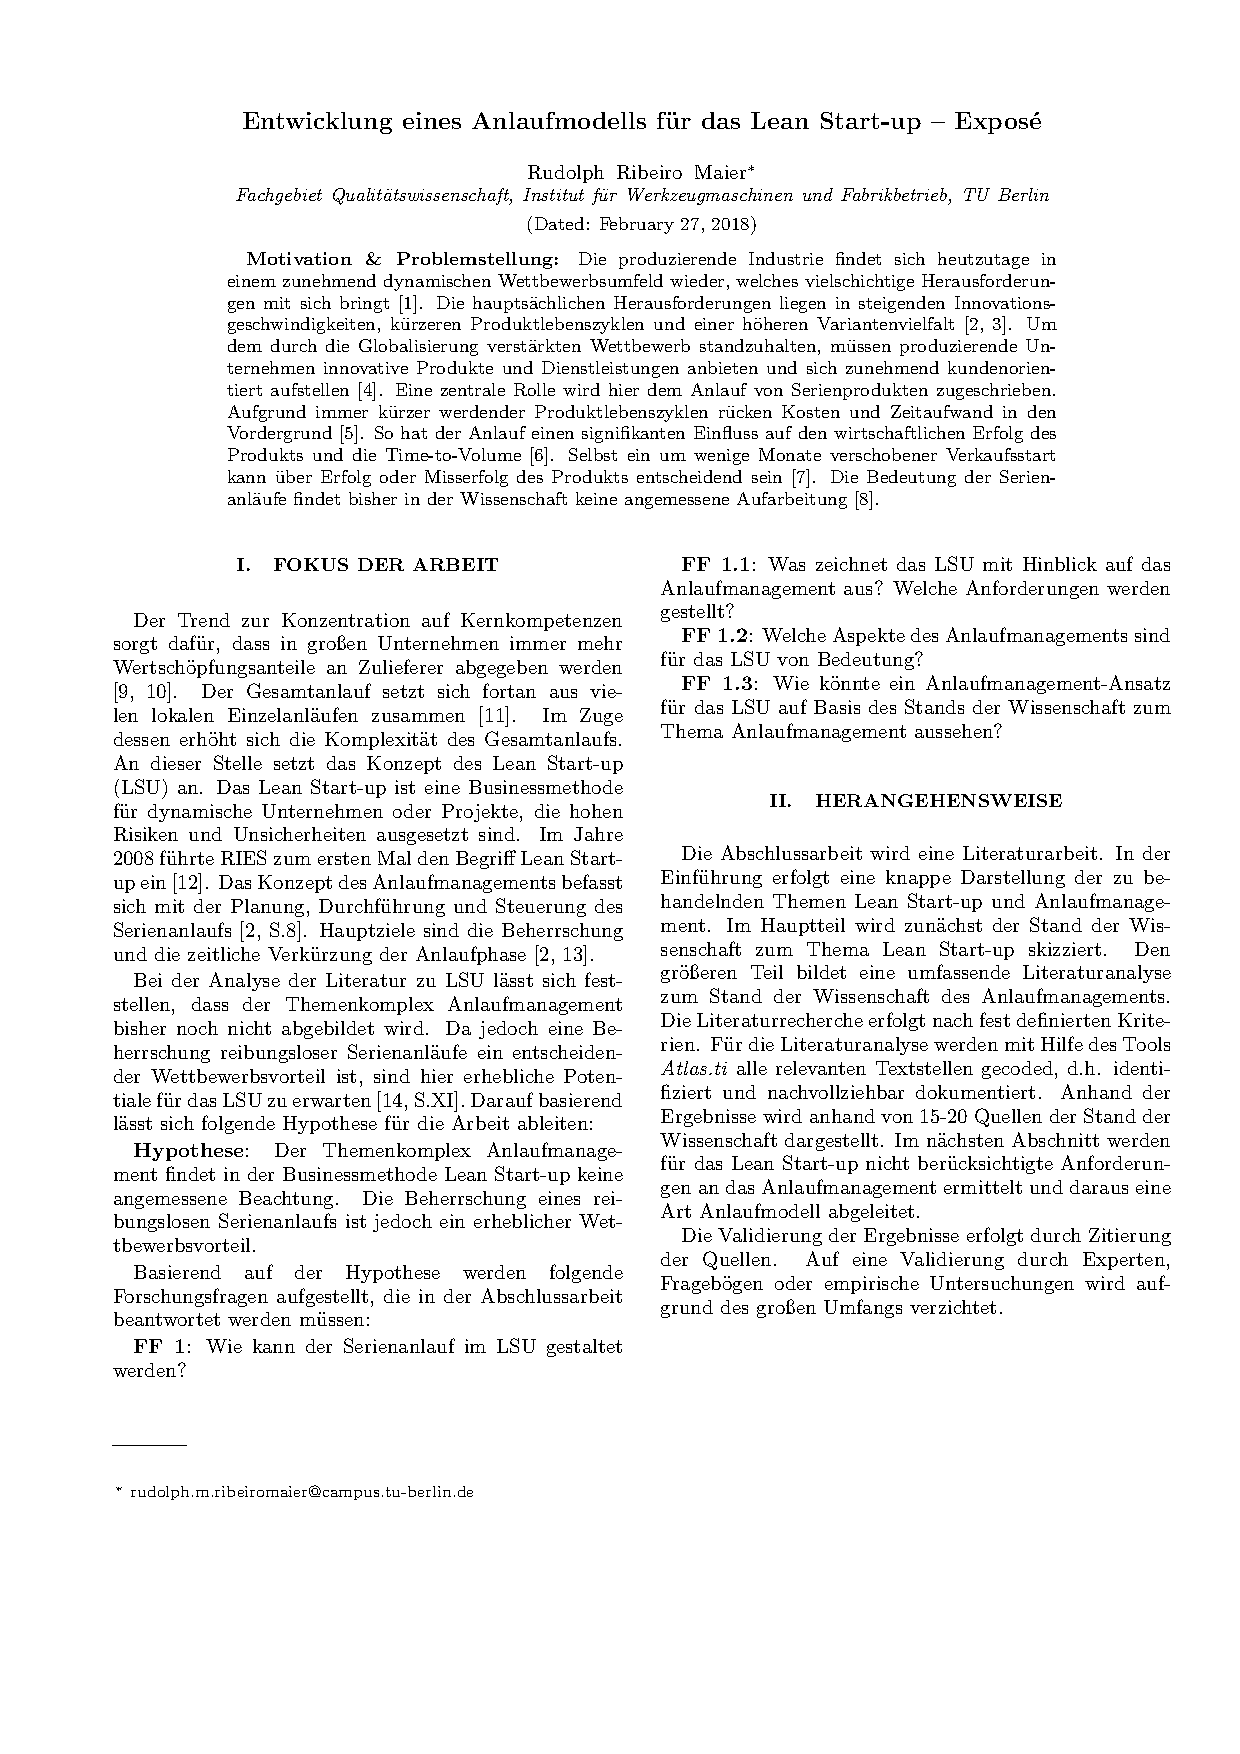
\includepdf[pages={1,2}]{latex_settings/onepager.pdf}			% Aufgabenstellung

% \chapter{Ergänzungen}
\newgeometry{left=30mm, right=30mm, top=20mm, bottom=5mm}
\section{Die Entwicklung des Grundgerüsts}
\begin{figure}[ht]
 \centering
 \includegraphics[scale=.76,clip=true,trim=30 50 30 40]{./img/Kollage.pdf}
 % Kollage.pdf: 0x0 pixel, 300dpi, 0.00x0.00 cm, bb=
 \caption{Entwicklung des Grundgerüsts}
 \label{fig:kollage}
\end{figure}

\clearpage
\restoregeometry

\section{Dombrowski-2011a - Lean Ramp-up. Handlungs- und Gestaltungsfelder}
\subsection*{Die Handlungsfelder im Lean Ramp-up}\label{appendix:dom11a:hf}
\begin{description}

\item[Produktentwicklung und Konstruktion]
umfassen alle Aufgaben, die sich mit
dem Konzipieren, Entwerfen, Ausarbeiten und Erproben eines Produkts
beschäftigen. Als Ergebnis resultieren Zeichnungen, Stücklisten und andere Produktdokumentationen.

\item[Fertigungs- und Montagemittel] umfassen alle Aufgaben, die sich mit der Bedarfsplanung, Auswahl, Beschaffung,
Herstellung, Einrichtung, Programmierung und Inbetriebnahme von Maschinen, Anlagen, Werkzeugen und
Vorrichtungen beschäftigen. Dazu gehören auch die Wartung und Instandhaltung. Als Ergebnis resultiert ein
Fertigungs- und Montagekonzept.

\item[Fertigungs- und Montageprozesse] umfassen alle Aufgaben, die sich mit der
Festlegung der Arbeitsabläufe zur
Herstellung eines Produkts in der
Fertigung und Montage beschäftigen.
Es werden u. a. Reihenfolgen und
Vorgabezeiten bestimmt sowie Produktionsmittel zugeordnet. Als Ergebnis resultieren Arbeitspläne, in
denen alle Informationen dokumentiert sind.

\item[Personal- und Arbeitsorganisation] umfasst alle Aufgaben, die sich mit der
Bedarfs- und Einsatzplanung, Beschaffung, Entwicklung und Freisetzung von Personal sowie mit der Gestaltung einer arbeitsgerechten und
bestmöglichen Zusammenarbeit von
Mensch und Technik beschäftigen.
Als Ergebnis resultieren zum Beispiel
Personaleinsatzpläne,
 Arbeitszeitund Entgeltsysteme.

\item[Produktionsplanung und -steuerung]
(PPS) umfasst alle Aufgaben, die sich
mit der Festlegung, Veranlassung,
Überwachung und Sicherung des Produktionsprogramms nach Art und
Menge unter Berücksichtigung von
Terminen und Kapazitäten beschäftigen. Als Ergebnis resultiert ein Produktionsplan mit Bedarfsmengen und
-terminen für Zukauf- und Eigenfertigungsteile.

 \item[Einkaufs- und Dispositionsprozesse]
umfassen alle Aufgaben, die sich mit
der kostenoptimalen strategischen
und operativen Beschaffung von Zukaufteilen, Handelswaren, Betriebsmitteln und Dienstleistungen von einem Lieferanten beschäftigen. Als Ergebnis resultieren zum Beispiel Sourcingstrategien, Verträge mit Lieferanten und verfügbare Lagerbestände.


 \item[Logistikprozesse und Logistikmittel]
umfassen alle Aufgaben, die sich mit
der Festlegung von effizienten inner-
und außerbetrieblichen Transporten
bzw. Materialflüssen und der Bereitstellung von Gütern beschäftigen.
Außerdem werden Logistikmittel, wie
z. B. Lager- und Transportmittel bestimmt. Als Ergebnis resultieren sog.
Logistiksysteme.

 \item[Gebäude, Layout und Arbeitsplätze]
umfassen alle fabrikplanerischen Aufgaben, die sich mit der Festlegung, optimalen Auslegung und Realisierung
der Produktionsstätten beschäftigen.
Der Umfang reicht dabei von der Umgestaltung einzelner Arbeitsplätze bis
hin zur Errichtung neuer Gebäude.
Als Ergebnis resultieren eingerichtete
Arbeitsplätze, Flächen und Gebäude.


 \item[Qualitätsmanagement und Qualitätsmittel] umfassen alle Aufgaben, die
sich mit der Planung, Lenkung, Prüfung, Sicherung und Verbesserung
der Qualitätsmerkmale von Produkten, Prozessen und Leistungen beschäftigen. Außerdem werden Qualitätsmittel, wie z. B. Prüf- und Messmittel bestimmt. Als Ergebnis resultieren beispielsweise Arbeits- und
Prüfanweisungen.

\item[Informationsprozesse und -systeme]
umfassen alle Aufgaben, die sich mit
der Beschaffung, Verarbeitung, Übertragung und Speicherung von Informationen zur Integration und zielorientierten Steuerung aller operativen Prozesse beschäftigen. Als Ergebnis resultieren zum Beispiel Systeme
zur Betriebsdatenerfassung (BDE).
\end{description}

\subsection*{Die Gestaltungsfelder im Lean Ramp-up}\label{appendix:dom11a:gf}
\begin{description}
\item[Integration und Kooperation] umfassen
alle Methoden und Werkzeuge, die
fachbereichs-, phasen"~, technologie- und unternehmensübergreifend zur
Synchronisierung von Produkt- und
Produktionsentwicklung beitragen.
Dazu wird eine simultane, interdisziplinäre und partnerschaftliche Zusammenarbeit angestrebt. Ziel ist es,
zum Beispiel Schnittstellen und Änderungen zu reduzieren.

\item[Partizipation und Veränderung] umfassen alle Methoden und Werkzeuge,
die zur Motivation der Mitarbeiter
und zum Abbau bzw. zur Vermeidung
von Widerständen und Konflikten beitragen. Dazu werden alle betroffenen
Organisationseinheiten am ProdukBild 4. Gestaltungsfelder im Lean Ramp-up
tionsanlauf beteiligt. Ziel ist es, die
Potenziale der Mitarbeiter zu nutzen
und einen reibungslosen Anlauf zu erreichen.

 \item[Wertschöpfung und Just-in-Time (JIT)]
umfassen alle Methoden und Werkzeuge, die zur produktiven, schnellen
und termingerechten Herstellung
bzw. Lieferung der Produkte beitragen. Dazu werden alle Verluste in den
Produktions- und Logistikprozessen
eliminiert und eine fließende und
kundenorientierte Produktion aufgebaut. Ziel ist ein schlankes Produktionssystem.

 \item[Pilotierung und Qualifizierung] umfasst
alle Methoden und Werkzeuge, die
zur Absicherung von Produkt- und
Prozessreifegrad sowie zur Steigerung der Leistungsfähigkeit des Produktionssystems beitragen. Dazu
werden sog. Pilotbereiche eingerichtet in denen Produktionstests sowie
Mitarbeiterschulungen erfolgen. Ziel
ist eine steile Lern- bzw. Anlaufkurve.

 \item[Priorisierung und Standardisierung]
umfassen alle Methoden und Werkzeuge, die zur Reduzierung, Beherrschung und Vermeidung der technologischen, prozessualen und organisatorischen Komplexität im Produktionsanlauf beitragen. Dazu werden
Schwerpunkte gebildet und Referenzunterlagen erstellt. Ziel ist es, den
Aufwand im Produktionsanlauf zu reduzieren.

 \item[Reaktionsfähigkeit und Flexibilität] umfassen alle Methoden und Werkzeuge,
die zum zeitnahen Erkennen veränderter Randbedingungen und Störungen sowie zur kontinuierlichen Anpassung des Anlaufmanagements beitragen. Dazu werden Frühwarnsysteme etabliert und Handlungsoptionen
bestimmt. Ziel ist es, schnell auf Veränderungen und Störungen zu reagieren.

 \item[Fehler- und Risikovermeidung] umfasst
alle Methoden und Werkzeuge, die
zur präventiven Qualitätssicherung
und -verbesserung beitragen. Dazu
werden frühzeitig die Ergebnisse der
Produkt- und Produktionsentwicklung veranschaulicht und Fehler- bzw.
Risikopotentiale eliminiert. Ziel sind
eine hohe Produkt- und Prozessqualität sowie geringe Änderungs- und
Prüfkosten.

 \item[Problemlösung und Stabilisierung] umfassen alle Methoden und Werkzeuge,
die zur reaktiven Qualitätssicherung
und -verbesserung beitragen. Dazu
werden die Produkte und Prozesse
kontinuierlich überprüft und überwacht sowie systematisch Problemursachen beseitigt. Ziel ist eine Stabilisierung des Anlaufs und Vermeidung
von Folge- und Wiederholungsfehlern.

 \item[Wissenstransfer und KVP] umfassen
alle Methoden und Werkzeuge, die
zum Transfer von Erfahrungswissen
und zur Erhöhung der Mitarbeiterkompetenzen beitragen. Dazu wird
explizites und – soweit möglich – implizites Wissen identifiziert, gesammelt, aufbereitet und vermittelt. Ziel
ist es, mit dessen Nutzung und
Weiterentwicklung aktuelle und zukünftige Anläufe zu verbessern.

 \item[Transparenz und Visualisierung] umfassen alle Methoden und Werkzeuge,
die zur Verfügbarkeit und leicht verständlichen Darstellung von Informationen und Daten beitragen. Dazu
werden sowohl informations- und
kommunikationstechnische Systeme
als auch optische Hilfsmittel und Signale eingesetzt. Ziel ist die Regelung,
Steuerung und Verbesserung des Produktionsanlaufs.
\end{description}


\newpage
%   left=30mm, right=30mm, top=20mm, bottom=20mm, % margins

\newgeometry{left=30mm, right=30mm, top=20mm, bottom=5mm}
\section{Dombrowski-2011b - Lean Ramp-up: Schwerpunkte im Anlaufmanagement}
\begin{figure}[h!]
 \centering
 \includegraphics[scale=.3]{./img/dom11b:firstmover.png}
 % dom11b:firstmover.png: 0x0 pixel, 0dpi, 0.00x0.00 cm, bb=
 \caption[Schwerpunkte für \textit{Firstmover}]{Schwerpunkte für \textit{Firstmover} \autocite{Dombrowski2011b}}
 \label{fig:dom11b:firstmover}
 \vspace{8mm}
% \end{figure}
% 
% 
% \begin{figure}[h]
 \centering
 \includegraphics[scale=.3]{./img/dom11b:kostenfuehrer.png}
 % dom11b:firstmover.png: 0x0 pixel, 0dpi, 0.00x0.00 cm, bb=
 \caption[Schwerpunkte für \textit{Follower (Kosten)}]{Schwerpunkte für \textit{Follower (Kosten)} \autocite{Dombrowski2011b}}
 \label{fig:dom11b:kostenfuehrer}
 \vspace{8mm}
% \end{figure}
% 
% 
% \begin{figure}[h]
 \centering
 \includegraphics[scale=.3]{./img/dom11b:qualitaetsfuehrer.png}
 % dom11b:firstmover.png: 0x0 pixel, 0dpi, 0.00x0.00 cm, bb=
 \caption[Schwerpunkte für \textit{Follower (Qualität)}]{Schwerpunkte für \textit{Follower (Qualität)} \autocite{Dombrowski2011b}}
 \label{fig:dom11b:qualitaetsfuehrer}
%  \vspace{5mm}
\end{figure}
\restoregeometry  
\newpage
\blankpage
\end{document}
